\documentclass[twoside]{book}

% Packages required by doxygen
\usepackage{fixltx2e}
\usepackage{calc}
\usepackage{doxygen}
\usepackage[export]{adjustbox} % also loads graphicx
\usepackage{graphicx}
\usepackage[utf8]{inputenc}
\usepackage{makeidx}
\usepackage{multicol}
\usepackage{multirow}
\PassOptionsToPackage{warn}{textcomp}
\usepackage{textcomp}
\usepackage[nointegrals]{wasysym}
\usepackage[table]{xcolor}

% NLS support packages
\usepackage[french]{babel}

% Font selection
\usepackage[T1]{fontenc}
\usepackage[scaled=.90]{helvet}
\usepackage{courier}
\usepackage{amssymb}
\usepackage{sectsty}
\renewcommand{\familydefault}{\sfdefault}
\allsectionsfont{%
  \fontseries{bc}\selectfont%
  \color{darkgray}%
}
\renewcommand{\DoxyLabelFont}{%
  \fontseries{bc}\selectfont%
  \color{darkgray}%
}
\newcommand{\+}{\discretionary{\mbox{\scriptsize$\hookleftarrow$}}{}{}}

% Page & text layout
\usepackage{geometry}
\geometry{%
  a4paper,%
  top=2.5cm,%
  bottom=2.5cm,%
  left=2.5cm,%
  right=2.5cm%
}
\tolerance=750
\hfuzz=15pt
\hbadness=750
\setlength{\emergencystretch}{15pt}
\setlength{\parindent}{0cm}
\setlength{\parskip}{0.2cm}
\makeatletter
\renewcommand{\paragraph}{%
  \@startsection{paragraph}{4}{0ex}{-1.0ex}{1.0ex}{%
    \normalfont\normalsize\bfseries\SS@parafont%
  }%
}
\renewcommand{\subparagraph}{%
  \@startsection{subparagraph}{5}{0ex}{-1.0ex}{1.0ex}{%
    \normalfont\normalsize\bfseries\SS@subparafont%
  }%
}
\makeatother

% Headers & footers
\usepackage{fancyhdr}
\pagestyle{fancyplain}
\fancyhead[LE]{\fancyplain{}{\bfseries\thepage}}
\fancyhead[CE]{\fancyplain{}{}}
\fancyhead[RE]{\fancyplain{}{\bfseries\leftmark}}
\fancyhead[LO]{\fancyplain{}{\bfseries\rightmark}}
\fancyhead[CO]{\fancyplain{}{}}
\fancyhead[RO]{\fancyplain{}{\bfseries\thepage}}
\fancyfoot[LE]{\fancyplain{}{}}
\fancyfoot[CE]{\fancyplain{}{}}
\fancyfoot[RE]{\fancyplain{}{\bfseries\scriptsize Généré le Vendredi 18 Décembre 2015 10\+:22\+:01 pour Tactics Arena par Doxygen }}
\fancyfoot[LO]{\fancyplain{}{\bfseries\scriptsize Généré le Vendredi 18 Décembre 2015 10\+:22\+:01 pour Tactics Arena par Doxygen }}
\fancyfoot[CO]{\fancyplain{}{}}
\fancyfoot[RO]{\fancyplain{}{}}
\renewcommand{\footrulewidth}{0.4pt}
\renewcommand{\chaptermark}[1]{%
  \markboth{#1}{}%
}
\renewcommand{\sectionmark}[1]{%
  \markright{\thesection\ #1}%
}

% Indices & bibliography
\usepackage{natbib}
\usepackage[titles]{tocloft}
\setcounter{tocdepth}{3}
\setcounter{secnumdepth}{5}
\makeindex

% Hyperlinks (required, but should be loaded last)
\usepackage{ifpdf}
\ifpdf
  \usepackage[pdftex,pagebackref=true]{hyperref}
\else
  \usepackage[ps2pdf,pagebackref=true]{hyperref}
\fi
\hypersetup{%
  colorlinks=true,%
  linkcolor=blue,%
  citecolor=blue,%
  unicode%
}

% Custom commands
\newcommand{\clearemptydoublepage}{%
  \newpage{\pagestyle{empty}\cleardoublepage}%
}


%===== C O N T E N T S =====

\begin{document}

% Titlepage & ToC
\hypersetup{pageanchor=false,
             bookmarks=true,
             bookmarksnumbered=true,
             pdfencoding=unicode
            }
\pagenumbering{roman}
\begin{titlepage}
\vspace*{7cm}
\begin{center}%
{\Large Tactics Arena }\\
\vspace*{1cm}
{\large Généré par Doxygen 1.8.9.1}\\
\vspace*{0.5cm}
{\small Vendredi 18 Décembre 2015 10:22:01}\\
\end{center}
\end{titlepage}
\clearemptydoublepage
\tableofcontents
\clearemptydoublepage
\pagenumbering{arabic}
\hypersetup{pageanchor=true}

%--- Begin generated contents ---
\chapter{Page principale}
\label{index}\hypertarget{index}{}Tactics Arena est un jeu de stratégie au tour par tour se jouant sur un plateau. Chaque joueur déplace ses unités respectant des règles de déplacement propre à chaque unité, le but du jeu est d\textquotesingle{}éliminer ou paralyser toutes les unités ennemies.

\subsection*{Règles}

Les conditions d\textquotesingle{}égalité sont\+:


\begin{DoxyItemize}
\item {\bfseries Toutes les unités actives sont détruites ou immobilisée}
\item {\bfseries Les joueurs passent leurs tours 3 fois d’affilé}
\item {\bfseries Il n’y a eu aucune rencontre entre les deux unités ennemies depuis les 30 derniers tours.}
\end{DoxyItemize}

Le joueur qui commence est défini aléatoirement par l\textquotesingle{}ordinateur au début de chaque partie.

Il n\textquotesingle{}est possible de déplacer qu\textquotesingle{}une seule unité par tour soit pour\+:


\begin{DoxyEnumerate}
\item {\bfseries Se déplacer}
\item {\bfseries Et / ou attaquer}
\item {\bfseries Et / ou changer de direction}
\end{DoxyEnumerate}

Le changement de direction impose d\textquotesingle{}être fait en dernier.

Chaque tour dure 1 à 2 minutes, dépendant du nombre d\textquotesingle{}unité restante. Une fois ce temps expiré\+:


\begin{DoxyItemize}
\item {\bfseries Le tour se termine automatiquement si au moins une commande a été effectué}
\item {\bfseries Si aucune commande n\textquotesingle{}a été effectuée alors abandon automatique}
\end{DoxyItemize}

\paragraph*{Important \+: toute action est irréversible.}

\subsection*{Sommaire}

{\bfseries Tactics Arena}


\begin{DoxyEnumerate}
\item $\ast$$\ast$\href{#markdown-header-regles}{\tt Règles}$\ast$$\ast$
\item $\ast$$\ast$\href{#markdown-header-changelog}{\tt Changelog}$\ast$$\ast$
\begin{DoxyItemize}
\item $\ast$$\ast$\href{#markdown-header-version-01}{\tt Version 0.\+1}$\ast$$\ast$
\end{DoxyItemize}
\item $\ast$$\ast$\href{#markdown-header-a-faire}{\tt A faire}$\ast$$\ast$
\item $\ast$$\ast$\href{#markdown-header-instructions-de-compilation}{\tt Instructions de compilation}$\ast$$\ast$
\item $\ast$$\ast$\href{#markdown-header-utilisation}{\tt Utilisation}$\ast$$\ast$
\item $\ast$$\ast$\href{#markdown-header-documentation}{\tt Documentation}$\ast$$\ast$
\end{DoxyEnumerate}

\subsection*{A faire}


\begin{DoxyItemize}
\item $\ast$$\ast$\mbox{[}x\mbox{]} Analyse préliminaire$\ast$$\ast$
\item $\ast$$\ast$\mbox{[} \mbox{]} Compte rendu mécaniques du jeu$\ast$$\ast$
\item $\ast$$\ast$\mbox{[}x\mbox{]} Analyse conceptuelle$\ast$$\ast$
\item $\ast$$\ast$\mbox{[} \mbox{]} Implémentation$\ast$$\ast$
\begin{DoxyItemize}
\item $\ast$$\ast$\mbox{[}x\mbox{]} Grille$\ast$$\ast$
\item $\ast$$\ast$\mbox{[}x\mbox{]} Menu$\ast$$\ast$
\item $\ast$$\ast$\mbox{[}x\mbox{]} Unités$\ast$$\ast$
\item $\ast$$\ast$\mbox{[}x\mbox{]} Statistiques$\ast$$\ast$
\item $\ast$$\ast$\mbox{[} \mbox{]} Mouvements$\ast$$\ast$
\item $\ast$$\ast$\mbox{[} \mbox{]} Gestion des tours$\ast$$\ast$
\item $\ast$$\ast$\mbox{[} \mbox{]} Gestion du temps$\ast$$\ast$
\item $\ast$$\ast$\mbox{[} \mbox{]} Capacités spéciales$\ast$$\ast$
\item $\ast$$\ast$\mbox{[} \mbox{]} Etat unités$\ast$$\ast$
\end{DoxyItemize}
\item $\ast$$\ast$\mbox{[} \mbox{]} Test unitaires$\ast$$\ast$
\item $\ast$$\ast$\mbox{[} \mbox{]} Test d\textquotesingle{}intégration$\ast$$\ast$
\item $\ast$$\ast$\mbox{[} \mbox{]} Ajout de fonctionnalités$\ast$$\ast$
\begin{DoxyItemize}
\item $\ast$$\ast$\mbox{[} \mbox{]} Intégration I\+A$\ast$$\ast$
\item $\ast$$\ast$\mbox{[} \mbox{]} G\+U\+I$\ast$$\ast$
\end{DoxyItemize}
\end{DoxyItemize}

\subsection*{Changelog}

\subsubsection*{Version 0.\+1}


\begin{DoxyItemize}
\item Mise en place sommaire des T\+A\+D
\end{DoxyItemize}

\subsection*{Instructions de compilation}

\subsection*{Utilisation}

\subsection*{Documentation}
\chapter{Index des classes}
\section{Liste des classes}
Liste des classes, structures, unions et interfaces avec une brève description \+:\begin{DoxyCompactList}
\item\contentsline{section}{\hyperlink{structelem}{elem} \\*Représente une case de la grille }{\pageref{structelem}}{}
\item\contentsline{section}{\hyperlink{structelement}{element} \\*Représente un élément de la liste }{\pageref{structelement}}{}
\item\contentsline{section}{\hyperlink{structtargetStat}{target\+Stat} \\*Représente les informations liées aux cibles }{\pageref{structtargetStat}}{}
\item\contentsline{section}{\hyperlink{structunit}{unit} \\*Représente une unité }{\pageref{structunit}}{}
\item\contentsline{section}{\hyperlink{structunitStat}{unit\+Stat} \\*Représente les statistiques d\textquotesingle{}une unité }{\pageref{structunitStat}}{}
\item\contentsline{section}{\hyperlink{structvector}{vector} \\*Représente les coordonnées d\textquotesingle{}un vecteur }{\pageref{structvector}}{}
\end{DoxyCompactList}

\chapter{Index des fichiers}
\section{Liste des fichiers}
Liste de tous les fichiers documentés avec une brève description \+:\begin{DoxyCompactList}
\item\contentsline{section}{include/controller/\hyperlink{manageSignal_8h}{manage\+Signal.\+h} \\*En-\/tête gestion des signaux }{\pageref{manageSignal_8h}}{}
\item\contentsline{section}{include/controller/\hyperlink{manageString_8h}{manage\+String.\+h} \\*En-\/tête gestion des chaînes de caractères }{\pageref{manageString_8h}}{}
\item\contentsline{section}{include/controller/\hyperlink{saveNLoad_8h}{save\+N\+Load.\+h} \\*En-\/tête gestion de la sauvegarde et chargement }{\pageref{saveNLoad_8h}}{}
\item\contentsline{section}{include/controller/\hyperlink{terminal_8h}{terminal.\+h} \\*En-\/tête gestion du terminal }{\pageref{terminal_8h}}{}
\item\contentsline{section}{include/display/\hyperlink{grid_8h}{grid.\+h} \\*En-\/tête gestion de la grille }{\pageref{grid_8h}}{}
\item\contentsline{section}{include/display/\hyperlink{menu_8h}{menu.\+h} \\*En-\/tête gestion des menus }{\pageref{menu_8h}}{}
\item\contentsline{section}{include/game/\hyperlink{engine_8h}{engine.\+h} \\*En-\/tête moteur de jeu }{\pageref{engine_8h}}{}
\item\contentsline{section}{include/game/\hyperlink{listes_8h}{listes.\+h} \\*En-\/tête listes de vecteurs }{\pageref{listes_8h}}{}
\item\contentsline{section}{include/game/\hyperlink{pathList_8h}{path\+List.\+h} \\*En-\/tête listes des chemins }{\pageref{pathList_8h}}{}
\item\contentsline{section}{include/game/\hyperlink{pawns_8h}{pawns.\+h} \\*En-\/tête gestions des pions }{\pageref{pawns_8h}}{}
\item\contentsline{section}{include/game/\hyperlink{turn_8h}{turn.\+h} \\*En-\/tête gestion des tours }{\pageref{turn_8h}}{}
\item\contentsline{section}{include/units/\hyperlink{unit_8h}{unit.\+h} \\*En-\/tête gestion des unités }{\pageref{unit_8h}}{}
\item\contentsline{section}{src/\hyperlink{main_8c}{main.\+c} \\*Programme principal }{\pageref{main_8c}}{}
\item\contentsline{section}{src/controller/\hyperlink{manageSignal_8c}{manage\+Signal.\+c} \\*Gestion des signaux }{\pageref{manageSignal_8c}}{}
\item\contentsline{section}{src/controller/\hyperlink{manageString_8c}{manage\+String.\+c} \\*Gestions des chaînes de caractères }{\pageref{manageString_8c}}{}
\item\contentsline{section}{src/controller/\hyperlink{saveNLoad_8c}{save\+N\+Load.\+c} \\*Gestion de la sauvegarde et du chargement }{\pageref{saveNLoad_8c}}{}
\item\contentsline{section}{src/controller/\hyperlink{terminal_8c}{terminal.\+c} \\*Gestion du terminal }{\pageref{terminal_8c}}{}
\item\contentsline{section}{src/display/\hyperlink{grid_8c}{grid.\+c} \\*Gestion de la grille }{\pageref{grid_8c}}{}
\item\contentsline{section}{src/display/\hyperlink{menu_8c}{menu.\+c} \\*Gestion des menus }{\pageref{menu_8c}}{}
\item\contentsline{section}{src/game/\hyperlink{engine_8c}{engine.\+c} \\*Moteur de jeu }{\pageref{engine_8c}}{}
\item\contentsline{section}{src/game/\hyperlink{listes_8c}{listes.\+c} \\*Listes de vecteurs }{\pageref{listes_8c}}{}
\item\contentsline{section}{src/game/\hyperlink{pathList_8c}{path\+List.\+c} \\*Listes de cases sur un chemin définis }{\pageref{pathList_8c}}{}
\item\contentsline{section}{src/game/\hyperlink{pawns_8c}{pawns.\+c} \\*Gestion des pions }{\pageref{pawns_8c}}{}
\item\contentsline{section}{src/game/\hyperlink{turn_8c}{turn.\+c} \\*Gestion des tours }{\pageref{turn_8c}}{}
\item\contentsline{section}{src/units/\hyperlink{unit_8c}{unit.\+c} \\*Gestion des unités }{\pageref{unit_8c}}{}
\end{DoxyCompactList}

\chapter{Documentation des classes}
\hypertarget{structelem}{}\section{Référence de la structure elem}
\label{structelem}\index{elem@{elem}}


Représente une case de la grille.  




{\ttfamily \#include $<$path\+List.\+c$>$}



Graphe de collaboration de elem\+:\nopagebreak
\begin{figure}[H]
\begin{center}
\leavevmode
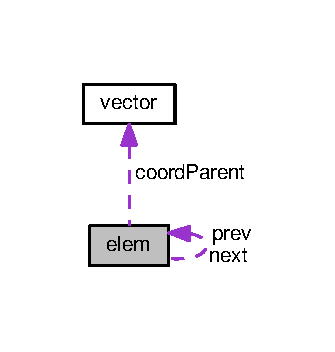
\includegraphics[width=161pt]{structelem__coll__graph}
\end{center}
\end{figure}
\subsection*{Attributs publics}
\begin{DoxyCompactItemize}
\item 
\hypertarget{structelem_a5460522be783257def1ac511288d74cb}{}\hyperlink{structvector}{vector} \hyperlink{structelem_a5460522be783257def1ac511288d74cb}{coord\+Parent}\label{structelem_a5460522be783257def1ac511288d74cb}

\begin{DoxyCompactList}\small\item\em Coordonnées de la case. \end{DoxyCompactList}\item 
\hypertarget{structelem_a000b7b27f503652106d30642ce3f40c2}{}int \hyperlink{structelem_a000b7b27f503652106d30642ce3f40c2}{F}\label{structelem_a000b7b27f503652106d30642ce3f40c2}

\begin{DoxyCompactList}\small\item\em Poids de la case. \end{DoxyCompactList}\item 
\hypertarget{structelem_aed06f2c7ef2050b131c8b72e099a0090}{}struct \hyperlink{structelem}{elem} $\ast$ \hyperlink{structelem_aed06f2c7ef2050b131c8b72e099a0090}{prev}\label{structelem_aed06f2c7ef2050b131c8b72e099a0090}

\begin{DoxyCompactList}\small\item\em Elément précédent. \end{DoxyCompactList}\item 
\hypertarget{structelem_ab9cf5c2e1c9a0ec2938275b90d39d5ca}{}struct \hyperlink{structelem}{elem} $\ast$ \hyperlink{structelem_ab9cf5c2e1c9a0ec2938275b90d39d5ca}{next}\label{structelem_ab9cf5c2e1c9a0ec2938275b90d39d5ca}

\begin{DoxyCompactList}\small\item\em Elément suivant. \end{DoxyCompactList}\end{DoxyCompactItemize}


\subsection{Description détaillée}
Représente une case de la grille. 

Définition à la ligne 16 du fichier path\+List.\+c.



La documentation de cette structure a été générée à partir du fichier suivant \+:\begin{DoxyCompactItemize}
\item 
src/game/\hyperlink{pathList_8c}{path\+List.\+c}\end{DoxyCompactItemize}

\hypertarget{structelement}{}\section{Référence de la structure element}
\label{structelement}\index{element@{element}}


Représente un élément de la liste.  




Graphe de collaboration de element\+:\nopagebreak
\begin{figure}[H]
\begin{center}
\leavevmode
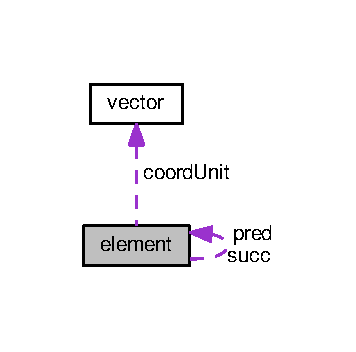
\includegraphics[width=171pt]{structelement__coll__graph}
\end{center}
\end{figure}
\subsection*{Attributs publics}
\begin{DoxyCompactItemize}
\item 
\hypertarget{structelement_a8a19f4b42fc45e4a8cfbff2d956e02d3}{}\hyperlink{structvector}{vector} \hyperlink{structelement_a8a19f4b42fc45e4a8cfbff2d956e02d3}{coord\+Unit}\label{structelement_a8a19f4b42fc45e4a8cfbff2d956e02d3}

\begin{DoxyCompactList}\small\item\em Coordonnées de l\textquotesingle{}unité \end{DoxyCompactList}\item 
\hypertarget{structelement_a9f9ebee1fa1dce6d05bc325a66478635}{}struct \hyperlink{structelement}{element} $\ast$ \hyperlink{structelement_a9f9ebee1fa1dce6d05bc325a66478635}{pred}\label{structelement_a9f9ebee1fa1dce6d05bc325a66478635}

\begin{DoxyCompactList}\small\item\em Élément précédent. \end{DoxyCompactList}\item 
\hypertarget{structelement_abe10f441a14a96bd130a004585b475ad}{}struct \hyperlink{structelement}{element} $\ast$ \hyperlink{structelement_abe10f441a14a96bd130a004585b475ad}{succ}\label{structelement_abe10f441a14a96bd130a004585b475ad}

\begin{DoxyCompactList}\small\item\em Élément suivant. \end{DoxyCompactList}\end{DoxyCompactItemize}


\subsection{Description détaillée}
Représente un élément de la liste. 

Définition à la ligne 19 du fichier listes.\+c.



La documentation de cette structure a été générée à partir du fichier suivant \+:\begin{DoxyCompactItemize}
\item 
src/game/\hyperlink{listes_8c}{listes.\+c}\end{DoxyCompactItemize}

\hypertarget{structtargetStat}{}\section{Référence de la structure target\+Stat}
\label{structtargetStat}\index{target\+Stat@{target\+Stat}}


Représente les informations liées aux cibles.  




{\ttfamily \#include $<$engine.\+h$>$}

\subsection*{Attributs publics}
\begin{DoxyCompactItemize}
\item 
\hypertarget{structtargetStat_a70d37dfedfb05d72d8c8cfcd575f812c}{}short \hyperlink{structtargetStat_a70d37dfedfb05d72d8c8cfcd575f812c}{vert\+Range}\label{structtargetStat_a70d37dfedfb05d72d8c8cfcd575f812c}

\begin{DoxyCompactList}\small\item\em Portée verticale. \end{DoxyCompactList}\item 
\hypertarget{structtargetStat_a2a4322825a13f8815c889056b123c09b}{}short \hyperlink{structtargetStat_a2a4322825a13f8815c889056b123c09b}{horiz\+Range}\label{structtargetStat_a2a4322825a13f8815c889056b123c09b}

\begin{DoxyCompactList}\small\item\em Portée horizontale. \end{DoxyCompactList}\item 
\hypertarget{structtargetStat_add6382059773722d55c40daff5b3efdc}{}short \hyperlink{structtargetStat_add6382059773722d55c40daff5b3efdc}{ring\+Size}\label{structtargetStat_add6382059773722d55c40daff5b3efdc}

\begin{DoxyCompactList}\small\item\em Taille de l\textquotesingle{}anneau. \end{DoxyCompactList}\item 
\hypertarget{structtargetStat_a178aadea19548628774763db12cdeb24}{}short \hyperlink{structtargetStat_a178aadea19548628774763db12cdeb24}{line}\label{structtargetStat_a178aadea19548628774763db12cdeb24}

\begin{DoxyCompactList}\small\item\em Ciblage en ligne. \end{DoxyCompactList}\end{DoxyCompactItemize}


\subsection{Description détaillée}
Représente les informations liées aux cibles. 

Définition à la ligne 54 du fichier engine.\+h.



La documentation de cette structure a été générée à partir du fichier suivant \+:\begin{DoxyCompactItemize}
\item 
include/game/\hyperlink{engine_8h}{engine.\+h}\end{DoxyCompactItemize}

\hypertarget{structunit}{}\section{Référence de la structure unit}
\label{structunit}\index{unit@{unit}}


Représente une unité  




{\ttfamily \#include $<$engine.\+h$>$}



Graphe de collaboration de unit\+:\nopagebreak
\begin{figure}[H]
\begin{center}
\leavevmode
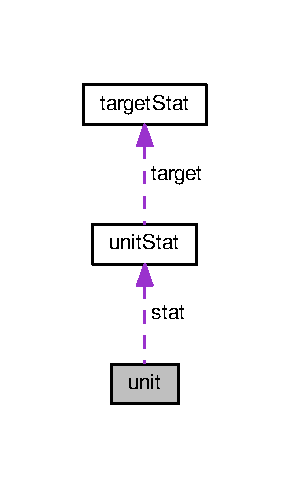
\includegraphics[width=139pt]{structunit__coll__graph}
\end{center}
\end{figure}
\subsection*{Attributs publics}
\begin{DoxyCompactItemize}
\item 
\hypertarget{structunit_aad8b083b6438d26e8aade384522e867c}{}\hyperlink{engine_8h_af7667555c2dcfbdd55ec3e9dd6a907ba}{unit\+Name} \hyperlink{structunit_aad8b083b6438d26e8aade384522e867c}{name}\label{structunit_aad8b083b6438d26e8aade384522e867c}

\begin{DoxyCompactList}\small\item\em Nom de l\textquotesingle{}unité \end{DoxyCompactList}\item 
\hypertarget{structunit_a88d6da278053824260f4f4987773b34f}{}\hyperlink{structunitStat}{unit\+Stat} \hyperlink{structunit_a88d6da278053824260f4f4987773b34f}{stat}\label{structunit_a88d6da278053824260f4f4987773b34f}

\begin{DoxyCompactList}\small\item\em Statistiques de l\textquotesingle{}unité \end{DoxyCompactList}\item 
\hypertarget{structunit_ab65f3e50337d201c634aa46587ea32ff}{}\hyperlink{engine_8h_ac5ece9b6993cd3565502866b56317e84}{unit\+Effect} \hyperlink{structunit_ab65f3e50337d201c634aa46587ea32ff}{effect} \mbox{[}\hyperlink{engine_8h_a21db47461d910a7cad180b5532f1a7f8}{N\+B\+\_\+\+M\+A\+X\+\_\+\+E\+F\+F\+E\+C\+T}\mbox{]}\label{structunit_ab65f3e50337d201c634aa46587ea32ff}

\begin{DoxyCompactList}\small\item\em Effets sur l\textquotesingle{}unité \end{DoxyCompactList}\item 
\hypertarget{structunit_a249f61ef45de3f8ca00b181374f2f051}{}\hyperlink{engine_8h_a468af3d7606639780e81c5e1e403b356}{cardinal} \hyperlink{structunit_a249f61ef45de3f8ca00b181374f2f051}{direct}\label{structunit_a249f61ef45de3f8ca00b181374f2f051}

\begin{DoxyCompactList}\small\item\em Direction de l\textquotesingle{}unité \end{DoxyCompactList}\item 
\hypertarget{structunit_a885e1b4b75d53199f4b03bdbd442cd37}{}int \hyperlink{structunit_a885e1b4b75d53199f4b03bdbd442cd37}{no\+Player}\label{structunit_a885e1b4b75d53199f4b03bdbd442cd37}

\begin{DoxyCompactList}\small\item\em Propriétaire de l\textquotesingle{}unité \end{DoxyCompactList}\item 
\hypertarget{structunit_abc126ccf502f7c7e7ec72e38b75c3e0e}{}int \hyperlink{structunit_abc126ccf502f7c7e7ec72e38b75c3e0e}{unit\+Color}\label{structunit_abc126ccf502f7c7e7ec72e38b75c3e0e}

\begin{DoxyCompactList}\small\item\em Couleur de l\textquotesingle{}unité \end{DoxyCompactList}\end{DoxyCompactItemize}


\subsection{Description détaillée}
Représente une unité 

Définition à la ligne 88 du fichier engine.\+h.



La documentation de cette structure a été générée à partir du fichier suivant \+:\begin{DoxyCompactItemize}
\item 
include/game/\hyperlink{engine_8h}{engine.\+h}\end{DoxyCompactItemize}

\hypertarget{structunitStat}{}\section{Référence de la structure unit\+Stat}
\label{structunitStat}\index{unit\+Stat@{unit\+Stat}}


Représente les statistiques d\textquotesingle{}une unité  




{\ttfamily \#include $<$engine.\+h$>$}



Graphe de collaboration de unit\+Stat\+:\nopagebreak
\begin{figure}[H]
\begin{center}
\leavevmode
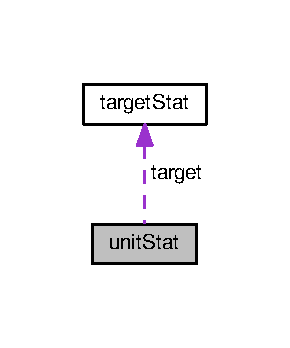
\includegraphics[width=139pt]{structunitStat__coll__graph}
\end{center}
\end{figure}
\subsection*{Attributs publics}
\begin{DoxyCompactItemize}
\item 
\hypertarget{structunitStat_aa11e3fe576364497283adf1140411079}{}int \hyperlink{structunitStat_aa11e3fe576364497283adf1140411079}{H\+P}\label{structunitStat_aa11e3fe576364497283adf1140411079}

\begin{DoxyCompactList}\small\item\em Points de vie. \end{DoxyCompactList}\item 
\hypertarget{structunitStat_a1e1bf1de283cf18aec14dd026ae9dc63}{}int \hyperlink{structunitStat_a1e1bf1de283cf18aec14dd026ae9dc63}{P\+O\+W\+E\+R}\label{structunitStat_a1e1bf1de283cf18aec14dd026ae9dc63}

\begin{DoxyCompactList}\small\item\em Puissance. \end{DoxyCompactList}\item 
\hypertarget{structunitStat_a9677dc9f6f59b4a873591a9e3d22125e}{}float \hyperlink{structunitStat_a9677dc9f6f59b4a873591a9e3d22125e}{A\+R\+M\+O\+R}\label{structunitStat_a9677dc9f6f59b4a873591a9e3d22125e}

\begin{DoxyCompactList}\small\item\em Armure. \end{DoxyCompactList}\item 
\hypertarget{structunitStat_a9f29568c1079efe25de0dc1b4246af94}{}int \hyperlink{structunitStat_a9f29568c1079efe25de0dc1b4246af94}{R\+E\+C\+O\+V\+E\+R\+Y}\label{structunitStat_a9f29568c1079efe25de0dc1b4246af94}

\begin{DoxyCompactList}\small\item\em Repos. \end{DoxyCompactList}\item 
\hypertarget{structunitStat_a9626453a4b1afd79a37b7c493280cbbd}{}float \hyperlink{structunitStat_a9626453a4b1afd79a37b7c493280cbbd}{B\+L\+O\+C\+K} \mbox{[}3\mbox{]}\label{structunitStat_a9626453a4b1afd79a37b7c493280cbbd}

\begin{DoxyCompactList}\small\item\em Blocage. \end{DoxyCompactList}\item 
\hypertarget{structunitStat_a344b6bf4fa47f6bd98073a0351dfb6bd}{}\hyperlink{structtargetStat}{target\+Stat} \hyperlink{structunitStat_a344b6bf4fa47f6bd98073a0351dfb6bd}{target}\label{structunitStat_a344b6bf4fa47f6bd98073a0351dfb6bd}

\begin{DoxyCompactList}\small\item\em Ciblage. \end{DoxyCompactList}\item 
\hypertarget{structunitStat_a4fb8a90b096d073d947c861a5536c2b9}{}int \hyperlink{structunitStat_a4fb8a90b096d073d947c861a5536c2b9}{M\+O\+V\+E\+\_\+\+R\+A\+N\+G\+E}\label{structunitStat_a4fb8a90b096d073d947c861a5536c2b9}

\begin{DoxyCompactList}\small\item\em Portée mouvement. \end{DoxyCompactList}\end{DoxyCompactItemize}


\subsection{Description détaillée}
Représente les statistiques d\textquotesingle{}une unité 

Définition à la ligne 65 du fichier engine.\+h.



La documentation de cette structure a été générée à partir du fichier suivant \+:\begin{DoxyCompactItemize}
\item 
include/game/\hyperlink{engine_8h}{engine.\+h}\end{DoxyCompactItemize}

\hypertarget{structvector}{}\section{Référence de la structure vector}
\label{structvector}\index{vector@{vector}}


Représente les coordonnées d\textquotesingle{}un vecteur.  




{\ttfamily \#include $<$engine.\+h$>$}

\subsection*{Attributs publics}
\begin{DoxyCompactItemize}
\item 
\hypertarget{structvector_a0403eb3aea23a3009e276fba1d317046}{}int \hyperlink{structvector_a0403eb3aea23a3009e276fba1d317046}{x}\label{structvector_a0403eb3aea23a3009e276fba1d317046}

\begin{DoxyCompactList}\small\item\em Position x. \end{DoxyCompactList}\item 
\hypertarget{structvector_aad6de640298eae97ca0a094db5aff477}{}int \hyperlink{structvector_aad6de640298eae97ca0a094db5aff477}{y}\label{structvector_aad6de640298eae97ca0a094db5aff477}

\begin{DoxyCompactList}\small\item\em Position y. \end{DoxyCompactList}\end{DoxyCompactItemize}


\subsection{Description détaillée}
Représente les coordonnées d\textquotesingle{}un vecteur. 

Définition à la ligne 79 du fichier engine.\+h.



La documentation de cette structure a été générée à partir du fichier suivant \+:\begin{DoxyCompactItemize}
\item 
include/game/\hyperlink{engine_8h}{engine.\+h}\end{DoxyCompactItemize}

\chapter{Documentation des fichiers}
\hypertarget{manageSignal_8h}{}\section{Référence du fichier include/controller/manage\+Signal.h}
\label{manageSignal_8h}\index{include/controller/manage\+Signal.\+h@{include/controller/manage\+Signal.\+h}}


En-\/tête gestion des signaux.  


Ce graphe montre quels fichiers incluent directement ou indirectement ce fichier \+:\nopagebreak
\begin{figure}[H]
\begin{center}
\leavevmode
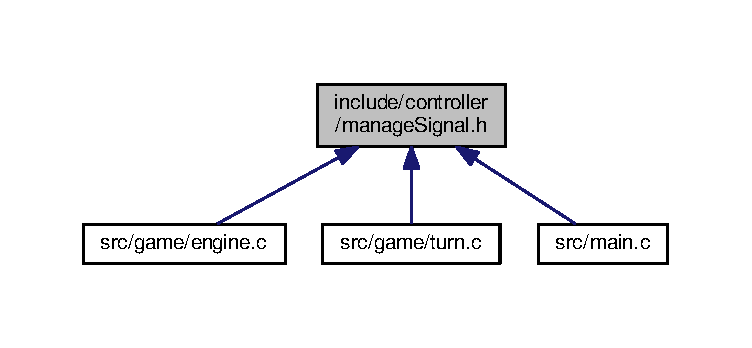
\includegraphics[width=350pt]{manageSignal_8h__dep__incl}
\end{center}
\end{figure}
\subsection*{Fonctions}
\begin{DoxyCompactItemize}
\item 
void \hyperlink{manageSignal_8h_a977fba31c29f9467d31b3efb9e0f8706}{check\+Signal} ()
\begin{DoxyCompactList}\small\item\em Vérifie les signaux du programme. \end{DoxyCompactList}\item 
\hypertarget{manageSignal_8h_a0bf71717b3a23473e63a11d8f5757afc}{}void \hyperlink{manageSignal_8h_a0bf71717b3a23473e63a11d8f5757afc}{time\+Down} ()\label{manageSignal_8h_a0bf71717b3a23473e63a11d8f5757afc}

\begin{DoxyCompactList}\small\item\em Message lors du temps écoulé \end{DoxyCompactList}\item 
void \hyperlink{manageSignal_8h_a91d6dcb4b4e4637a63aacf87b53132d0}{free\+All} ()
\begin{DoxyCompactList}\small\item\em Libère toute la mémoire. \end{DoxyCompactList}\end{DoxyCompactItemize}


\subsection{Description détaillée}
En-\/tête gestion des signaux. 

\begin{DoxyAuthor}{Auteur}
Cousin Brandon Chaudemanche Ewen Biardeau Tristan 
\end{DoxyAuthor}
\begin{DoxyVersion}{Version}
v1.\+00 
\end{DoxyVersion}
\begin{DoxyDate}{Date}
18/12/2015 
\end{DoxyDate}


\subsection{Documentation des fonctions}
\hypertarget{manageSignal_8h_a977fba31c29f9467d31b3efb9e0f8706}{}\index{manage\+Signal.\+h@{manage\+Signal.\+h}!check\+Signal@{check\+Signal}}
\index{check\+Signal@{check\+Signal}!manage\+Signal.\+h@{manage\+Signal.\+h}}
\subsubsection[{check\+Signal}]{\setlength{\rightskip}{0pt plus 5cm}void check\+Signal (
\begin{DoxyParamCaption}
{}
\end{DoxyParamCaption}
)}\label{manageSignal_8h_a977fba31c29f9467d31b3efb9e0f8706}


Vérifie les signaux du programme. 

Vérifie les signaux du programme. 

Définition à la ligne 77 du fichier manage\+Signal.\+c.

\hypertarget{manageSignal_8h_a91d6dcb4b4e4637a63aacf87b53132d0}{}\index{manage\+Signal.\+h@{manage\+Signal.\+h}!free\+All@{free\+All}}
\index{free\+All@{free\+All}!manage\+Signal.\+h@{manage\+Signal.\+h}}
\subsubsection[{free\+All}]{\setlength{\rightskip}{0pt plus 5cm}void free\+All (
\begin{DoxyParamCaption}
{}
\end{DoxyParamCaption}
)}\label{manageSignal_8h_a91d6dcb4b4e4637a63aacf87b53132d0}


Libère toute la mémoire. 

Libère toute la mémoire. 

Définition à la ligne 21 du fichier manage\+Signal.\+c.


\hypertarget{manageString_8h}{}\section{Référence du fichier include/controller/manage\+String.h}
\label{manageString_8h}\index{include/controller/manage\+String.\+h@{include/controller/manage\+String.\+h}}


En-\/tête gestion des chaînes de caractères.  


Ce graphe montre quels fichiers incluent directement ou indirectement ce fichier \+:\nopagebreak
\begin{figure}[H]
\begin{center}
\leavevmode
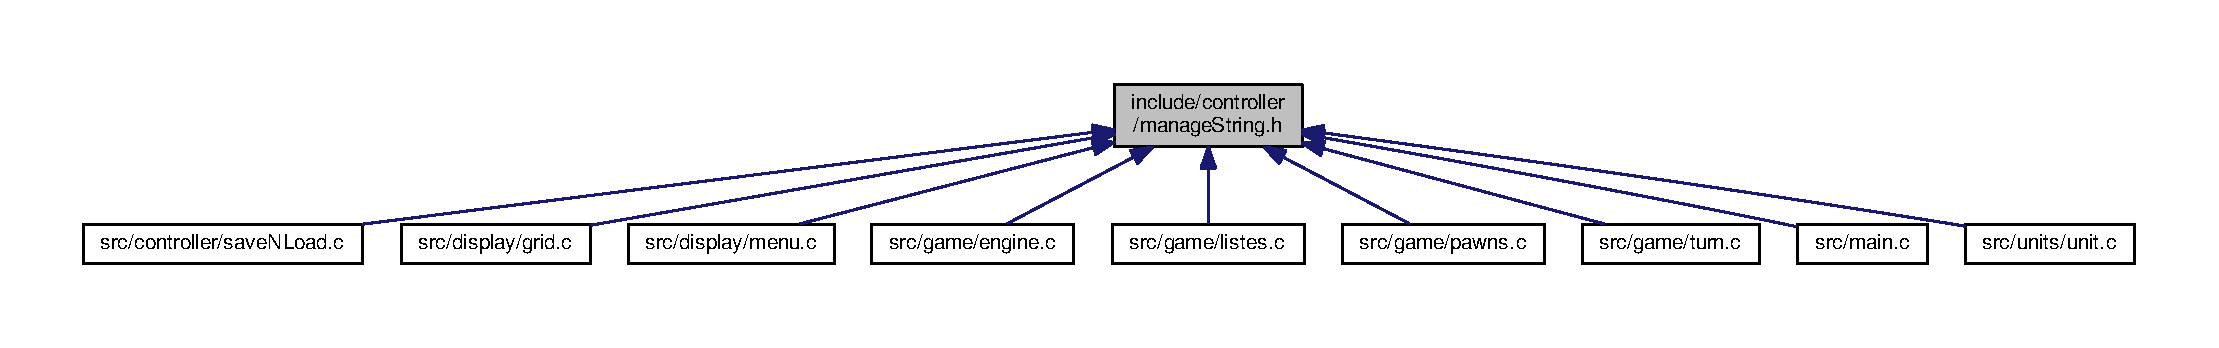
\includegraphics[width=350pt]{manageString_8h__dep__incl}
\end{center}
\end{figure}
\subsection*{Fonctions}
\begin{DoxyCompactItemize}
\item 
char $\ast$ \hyperlink{manageString_8h_aef4f9d954282d13b5ea3132465378b79}{get2\+Char} (char name\mbox{[}$\,$\mbox{]})
\begin{DoxyCompactList}\small\item\em Récupère 2 caractères du nom de l\textquotesingle{}unité \end{DoxyCompactList}\item 
char $\ast$ \hyperlink{manageString_8h_a1f1e45f2d8b8cf09e271c2459a46b0d3}{get\+Name\+Unit} (\hyperlink{engine_8h_af7667555c2dcfbdd55ec3e9dd6a907ba}{unit\+Name} \hyperlink{structunit}{unit})
\begin{DoxyCompactList}\small\item\em Récupère le nom de l\textquotesingle{}unité \end{DoxyCompactList}\item 
void \hyperlink{manageString_8h_a32a341ce2c2a9240c500f694c9227b96}{print\+Name\+Unit} (\hyperlink{engine_8h_af7667555c2dcfbdd55ec3e9dd6a907ba}{unit\+Name} \hyperlink{structunit}{unit})
\begin{DoxyCompactList}\small\item\em Affiche le nom de l\textquotesingle{}unité \end{DoxyCompactList}\item 
void \hyperlink{manageString_8h_a4660decf36a299266867a3fdffd4891f}{get\+Coord\+S} (char coord\+String\mbox{[}$\,$\mbox{]}, \hyperlink{structvector}{vector} $\ast$coord\+Unit)
\begin{DoxyCompactList}\small\item\em Récupère les coordonnées d\textquotesingle{}une chaîne de caractères. \end{DoxyCompactList}\item 
\hypertarget{manageString_8h_ab4002ec4f250e5f6b7f2b56936950b5e}{}bool \hyperlink{manageString_8h_ab4002ec4f250e5f6b7f2b56936950b5e}{correct\+Coord} (char $\ast$coord\+String)\label{manageString_8h_ab4002ec4f250e5f6b7f2b56936950b5e}

\begin{DoxyCompactList}\small\item\em Vérifie l\textquotesingle{}authenticité des coordonnées d\textquotesingle{}une chaîne de caractères. \end{DoxyCompactList}\item 
bool \hyperlink{manageString_8h_a56a4267e397f3c206d9655b52241024e}{right\+Side} (char $\ast$coord\+String)
\begin{DoxyCompactList}\small\item\em Vérifie que l\textquotesingle{}unité est dans le bon camp. \end{DoxyCompactList}\item 
int \hyperlink{manageString_8h_a57860307a2f1d8a80d71147a7ed1b793}{read\+S} (char $\ast$string)
\begin{DoxyCompactList}\small\item\em Lecture sécurisée d\textquotesingle{}une chaîne. \end{DoxyCompactList}\item 
long \hyperlink{manageString_8h_ab431b0689298bfb6b1e74cbe92c18e00}{read\+Long} ()
\begin{DoxyCompactList}\small\item\em Lecture sécurisée d\textquotesingle{}un long. \end{DoxyCompactList}\item 
double \hyperlink{manageString_8h_a840ea5c01770156bd51bdb9f65f44e30}{read\+Double} ()
\begin{DoxyCompactList}\small\item\em Lecture sécurisée d\textquotesingle{}un double. \end{DoxyCompactList}\item 
void \hyperlink{manageString_8h_a20bbd4d45e3f01305dd709f5a9cc9952}{clear\+Buffer} ()
\begin{DoxyCompactList}\small\item\em Vide la mémoire tampon. \end{DoxyCompactList}\item 
char $\ast$ \hyperlink{manageString_8h_a71644b2a2c56b83debb3c804040d3c88}{get\+Direction\+Unit} (\hyperlink{engine_8h_a468af3d7606639780e81c5e1e403b356}{cardinal} direct)
\begin{DoxyCompactList}\small\item\em Récupère le nom de la direction. \end{DoxyCompactList}\item 
char $\ast$ \hyperlink{manageString_8h_acb5c8162f1db822caca54e0e04d2a143}{get\+Name\+Effect} (\hyperlink{engine_8h_ac5ece9b6993cd3565502866b56317e84}{unit\+Effect} effect)
\begin{DoxyCompactList}\small\item\em Récupère le nom de l\textquotesingle{}effet. \end{DoxyCompactList}\end{DoxyCompactItemize}


\subsection{Description détaillée}
En-\/tête gestion des chaînes de caractères. 

\begin{DoxyAuthor}{Auteur}
Cousin Brandon Chaudemanche Ewen Biardeau Tristan 
\end{DoxyAuthor}
\begin{DoxyVersion}{Version}
v1.\+00 
\end{DoxyVersion}
\begin{DoxyDate}{Date}
18/12/2015 
\end{DoxyDate}


\subsection{Documentation des fonctions}
\hypertarget{manageString_8h_a20bbd4d45e3f01305dd709f5a9cc9952}{}\index{manage\+String.\+h@{manage\+String.\+h}!clear\+Buffer@{clear\+Buffer}}
\index{clear\+Buffer@{clear\+Buffer}!manage\+String.\+h@{manage\+String.\+h}}
\subsubsection[{clear\+Buffer}]{\setlength{\rightskip}{0pt plus 5cm}void clear\+Buffer (
\begin{DoxyParamCaption}
{}
\end{DoxyParamCaption}
)}\label{manageString_8h_a20bbd4d45e3f01305dd709f5a9cc9952}


Vide la mémoire tampon. 

Vide la mémoire tampon. 

Définition à la ligne 253 du fichier manage\+String.\+c.

\hypertarget{manageString_8h_aef4f9d954282d13b5ea3132465378b79}{}\index{manage\+String.\+h@{manage\+String.\+h}!get2\+Char@{get2\+Char}}
\index{get2\+Char@{get2\+Char}!manage\+String.\+h@{manage\+String.\+h}}
\subsubsection[{get2\+Char}]{\setlength{\rightskip}{0pt plus 5cm}char$\ast$ get2\+Char (
\begin{DoxyParamCaption}
\item[{char}]{name\mbox{[}$\,$\mbox{]}}
\end{DoxyParamCaption}
)}\label{manageString_8h_aef4f9d954282d13b5ea3132465378b79}


Récupère 2 caractères du nom de l\textquotesingle{}unité 


\begin{DoxyParams}{Paramètres}
{\em name} & Nom de l\textquotesingle{}unité \\
\hline
\end{DoxyParams}
\begin{DoxyReturn}{Renvoie}
Retourne 2 caractères liés au nom de l\textquotesingle{}unité 
\end{DoxyReturn}


Définition à la ligne 47 du fichier manage\+String.\+c.

\hypertarget{manageString_8h_a4660decf36a299266867a3fdffd4891f}{}\index{manage\+String.\+h@{manage\+String.\+h}!get\+Coord\+S@{get\+Coord\+S}}
\index{get\+Coord\+S@{get\+Coord\+S}!manage\+String.\+h@{manage\+String.\+h}}
\subsubsection[{get\+Coord\+S}]{\setlength{\rightskip}{0pt plus 5cm}void get\+Coord\+S (
\begin{DoxyParamCaption}
\item[{char}]{coord\+String\mbox{[}$\,$\mbox{]}, }
\item[{{\bf vector} $\ast$}]{coord\+Unit}
\end{DoxyParamCaption}
)}\label{manageString_8h_a4660decf36a299266867a3fdffd4891f}


Récupère les coordonnées d\textquotesingle{}une chaîne de caractères. 

Récupère les coordonnées d\textquotesingle{}une chaîne de caractères.


\begin{DoxyParams}{Paramètres}
{\em coord\+String} & Coordonnées saisie par l\textquotesingle{}utilisateur \\
\hline
{\em coord\+Unit} & Coordonnées de l\textquotesingle{}unité récupérées de la saisie utilisateur \\
\hline
\end{DoxyParams}


Définition à la ligne 19 du fichier manage\+String.\+c.

\hypertarget{manageString_8h_a71644b2a2c56b83debb3c804040d3c88}{}\index{manage\+String.\+h@{manage\+String.\+h}!get\+Direction\+Unit@{get\+Direction\+Unit}}
\index{get\+Direction\+Unit@{get\+Direction\+Unit}!manage\+String.\+h@{manage\+String.\+h}}
\subsubsection[{get\+Direction\+Unit}]{\setlength{\rightskip}{0pt plus 5cm}char$\ast$ get\+Direction\+Unit (
\begin{DoxyParamCaption}
\item[{{\bf cardinal}}]{direct}
\end{DoxyParamCaption}
)}\label{manageString_8h_a71644b2a2c56b83debb3c804040d3c88}


Récupère le nom de la direction. 

Récupère le nom de la direction.


\begin{DoxyParams}{Paramètres}
{\em direct} & Direction de l\textquotesingle{}unité \\
\hline
\end{DoxyParams}
\begin{DoxyReturn}{Renvoie}
Retourne La direction sous forme de chaîne 
\end{DoxyReturn}


Définition à la ligne 235 du fichier manage\+String.\+c.

\hypertarget{manageString_8h_acb5c8162f1db822caca54e0e04d2a143}{}\index{manage\+String.\+h@{manage\+String.\+h}!get\+Name\+Effect@{get\+Name\+Effect}}
\index{get\+Name\+Effect@{get\+Name\+Effect}!manage\+String.\+h@{manage\+String.\+h}}
\subsubsection[{get\+Name\+Effect}]{\setlength{\rightskip}{0pt plus 5cm}char$\ast$ get\+Name\+Effect (
\begin{DoxyParamCaption}
\item[{{\bf unit\+Effect}}]{effect}
\end{DoxyParamCaption}
)}\label{manageString_8h_acb5c8162f1db822caca54e0e04d2a143}


Récupère le nom de l\textquotesingle{}effet. 

Récupère le nom de l\textquotesingle{}effet.


\begin{DoxyParams}{Paramètres}
{\em effect} & Effet provenant de la liste énumérée \\
\hline
\end{DoxyParams}
\begin{DoxyReturn}{Renvoie}
Nom de l\textquotesingle{}effet sous forme de chaîne de caractère 
\end{DoxyReturn}


Définition à la ligne 220 du fichier manage\+String.\+c.

\hypertarget{manageString_8h_a1f1e45f2d8b8cf09e271c2459a46b0d3}{}\index{manage\+String.\+h@{manage\+String.\+h}!get\+Name\+Unit@{get\+Name\+Unit}}
\index{get\+Name\+Unit@{get\+Name\+Unit}!manage\+String.\+h@{manage\+String.\+h}}
\subsubsection[{get\+Name\+Unit}]{\setlength{\rightskip}{0pt plus 5cm}char$\ast$ get\+Name\+Unit (
\begin{DoxyParamCaption}
\item[{{\bf unit\+Name}}]{name}
\end{DoxyParamCaption}
)}\label{manageString_8h_a1f1e45f2d8b8cf09e271c2459a46b0d3}


Récupère le nom de l\textquotesingle{}unité 

Récupère le nom de l\textquotesingle{}unité


\begin{DoxyParams}{Paramètres}
{\em name} & Nom de l\textquotesingle{}unité provenant de la liste énumérée \\
\hline
\end{DoxyParams}
\begin{DoxyReturn}{Renvoie}
Nom de l\textquotesingle{}unité sous forme de chaîne 
\end{DoxyReturn}


Définition à la ligne 189 du fichier manage\+String.\+c.

\hypertarget{manageString_8h_a32a341ce2c2a9240c500f694c9227b96}{}\index{manage\+String.\+h@{manage\+String.\+h}!print\+Name\+Unit@{print\+Name\+Unit}}
\index{print\+Name\+Unit@{print\+Name\+Unit}!manage\+String.\+h@{manage\+String.\+h}}
\subsubsection[{print\+Name\+Unit}]{\setlength{\rightskip}{0pt plus 5cm}void print\+Name\+Unit (
\begin{DoxyParamCaption}
\item[{{\bf unit\+Name}}]{unit}
\end{DoxyParamCaption}
)}\label{manageString_8h_a32a341ce2c2a9240c500f694c9227b96}


Affiche le nom de l\textquotesingle{}unité 


\begin{DoxyParams}{Paramètres}
{\em unit} & Nom de l\textquotesingle{}unité provenant de la liste énumérée \\
\hline
\end{DoxyParams}


Définition à la ligne 246 du fichier manage\+String.\+c.

\hypertarget{manageString_8h_a840ea5c01770156bd51bdb9f65f44e30}{}\index{manage\+String.\+h@{manage\+String.\+h}!read\+Double@{read\+Double}}
\index{read\+Double@{read\+Double}!manage\+String.\+h@{manage\+String.\+h}}
\subsubsection[{read\+Double}]{\setlength{\rightskip}{0pt plus 5cm}double read\+Double (
\begin{DoxyParamCaption}
{}
\end{DoxyParamCaption}
)}\label{manageString_8h_a840ea5c01770156bd51bdb9f65f44e30}


Lecture sécurisée d\textquotesingle{}un double. 

Lecture sécurisée d\textquotesingle{}un double.

\begin{DoxyReturn}{Renvoie}
Retourne le double saisie ou 0.\+0 en cas d\textquotesingle{}erreur 
\end{DoxyReturn}


Définition à la ligne 305 du fichier manage\+String.\+c.

\hypertarget{manageString_8h_ab431b0689298bfb6b1e74cbe92c18e00}{}\index{manage\+String.\+h@{manage\+String.\+h}!read\+Long@{read\+Long}}
\index{read\+Long@{read\+Long}!manage\+String.\+h@{manage\+String.\+h}}
\subsubsection[{read\+Long}]{\setlength{\rightskip}{0pt plus 5cm}long read\+Long (
\begin{DoxyParamCaption}
{}
\end{DoxyParamCaption}
)}\label{manageString_8h_ab431b0689298bfb6b1e74cbe92c18e00}


Lecture sécurisée d\textquotesingle{}un long. 

Lecture sécurisée d\textquotesingle{}un long.

\begin{DoxyReturn}{Renvoie}
Retourne le long saisie ou 0 en cas d\textquotesingle{}erreur 
\end{DoxyReturn}


Définition à la ligne 291 du fichier manage\+String.\+c.

\hypertarget{manageString_8h_a57860307a2f1d8a80d71147a7ed1b793}{}\index{manage\+String.\+h@{manage\+String.\+h}!read\+S@{read\+S}}
\index{read\+S@{read\+S}!manage\+String.\+h@{manage\+String.\+h}}
\subsubsection[{read\+S}]{\setlength{\rightskip}{0pt plus 5cm}int read\+S (
\begin{DoxyParamCaption}
\item[{char $\ast$}]{string}
\end{DoxyParamCaption}
)}\label{manageString_8h_a57860307a2f1d8a80d71147a7ed1b793}


Lecture sécurisée d\textquotesingle{}une chaîne. 

Lecture sécurisée d\textquotesingle{}une chaîne.


\begin{DoxyParams}{Paramètres}
{\em string} & Chaîne de caractère à vérifier \\
\hline
\end{DoxyParams}
\begin{DoxyReturn}{Renvoie}
Retourne 1 si chaîne correcte 
\end{DoxyReturn}


Définition à la ligne 265 du fichier manage\+String.\+c.

\hypertarget{manageString_8h_a56a4267e397f3c206d9655b52241024e}{}\index{manage\+String.\+h@{manage\+String.\+h}!right\+Side@{right\+Side}}
\index{right\+Side@{right\+Side}!manage\+String.\+h@{manage\+String.\+h}}
\subsubsection[{right\+Side}]{\setlength{\rightskip}{0pt plus 5cm}bool right\+Side (
\begin{DoxyParamCaption}
\item[{char $\ast$}]{coord\+String}
\end{DoxyParamCaption}
)}\label{manageString_8h_a56a4267e397f3c206d9655b52241024e}


Vérifie que l\textquotesingle{}unité est dans le bon camp. 

Vérifie que l\textquotesingle{}unité est dans le bon camp.


\begin{DoxyParams}{Paramètres}
{\em coord\+String} & Coordonnées sous forme de chaîne \\
\hline
\end{DoxyParams}
\begin{DoxyReturn}{Renvoie}
Retourne vrai si du bon côté 
\end{DoxyReturn}


Définition à la ligne 165 du fichier manage\+String.\+c.


\hypertarget{saveNLoad_8h}{}\section{Référence du fichier include/controller/save\+N\+Load.h}
\label{saveNLoad_8h}\index{include/controller/save\+N\+Load.\+h@{include/controller/save\+N\+Load.\+h}}


En-\/tête gestion de la sauvegarde et chargement.  


Ce graphe montre quels fichiers incluent directement ou indirectement ce fichier \+:\nopagebreak
\begin{figure}[H]
\begin{center}
\leavevmode
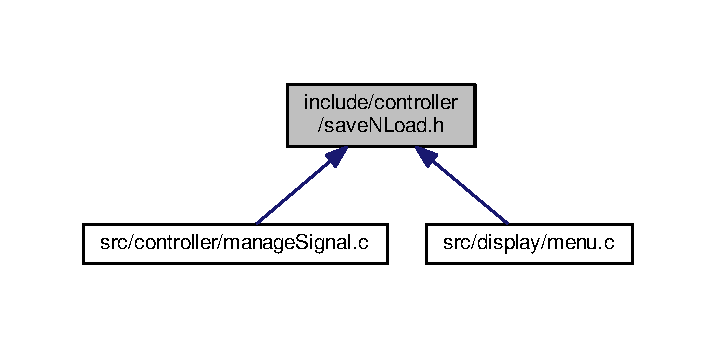
\includegraphics[width=344pt]{saveNLoad_8h__dep__incl}
\end{center}
\end{figure}
\subsection*{Fonctions}
\begin{DoxyCompactItemize}
\item 
void \hyperlink{saveNLoad_8h_aae2c382151ef7c9aa913361172b30db6}{save} ()
\begin{DoxyCompactList}\small\item\em Sauvegarde la partie. \end{DoxyCompactList}\item 
void \hyperlink{saveNLoad_8h_a78f61ac2dd03bcba8e09ca20cd7d68e3}{load} ()
\begin{DoxyCompactList}\small\item\em Charge une partie. \end{DoxyCompactList}\end{DoxyCompactItemize}


\subsection{Description détaillée}
En-\/tête gestion de la sauvegarde et chargement. 

\begin{DoxyAuthor}{Auteur}
Cousin Brandon Chaudemanche Ewen Biardeau Tristan 
\end{DoxyAuthor}
\begin{DoxyVersion}{Version}
v1.\+00 
\end{DoxyVersion}
\begin{DoxyDate}{Date}
18/12/2015 
\end{DoxyDate}


\subsection{Documentation des fonctions}
\hypertarget{saveNLoad_8h_a78f61ac2dd03bcba8e09ca20cd7d68e3}{}\index{save\+N\+Load.\+h@{save\+N\+Load.\+h}!load@{load}}
\index{load@{load}!save\+N\+Load.\+h@{save\+N\+Load.\+h}}
\subsubsection[{load}]{\setlength{\rightskip}{0pt plus 5cm}void load (
\begin{DoxyParamCaption}
{}
\end{DoxyParamCaption}
)}\label{saveNLoad_8h_a78f61ac2dd03bcba8e09ca20cd7d68e3}


Charge une partie. 

Charge une partie. 

Définition à la ligne 201 du fichier save\+N\+Load.\+c.

\hypertarget{saveNLoad_8h_aae2c382151ef7c9aa913361172b30db6}{}\index{save\+N\+Load.\+h@{save\+N\+Load.\+h}!save@{save}}
\index{save@{save}!save\+N\+Load.\+h@{save\+N\+Load.\+h}}
\subsubsection[{save}]{\setlength{\rightskip}{0pt plus 5cm}void save (
\begin{DoxyParamCaption}
{}
\end{DoxyParamCaption}
)}\label{saveNLoad_8h_aae2c382151ef7c9aa913361172b30db6}


Sauvegarde la partie. 

Sauvegarde la partie. 

Définition à la ligne 158 du fichier save\+N\+Load.\+c.


\hypertarget{terminal_8h}{}\section{Référence du fichier include/controller/terminal.h}
\label{terminal_8h}\index{include/controller/terminal.\+h@{include/controller/terminal.\+h}}


En-\/tête gestion du terminal.  


Ce graphe montre quels fichiers incluent directement ou indirectement ce fichier \+:\nopagebreak
\begin{figure}[H]
\begin{center}
\leavevmode
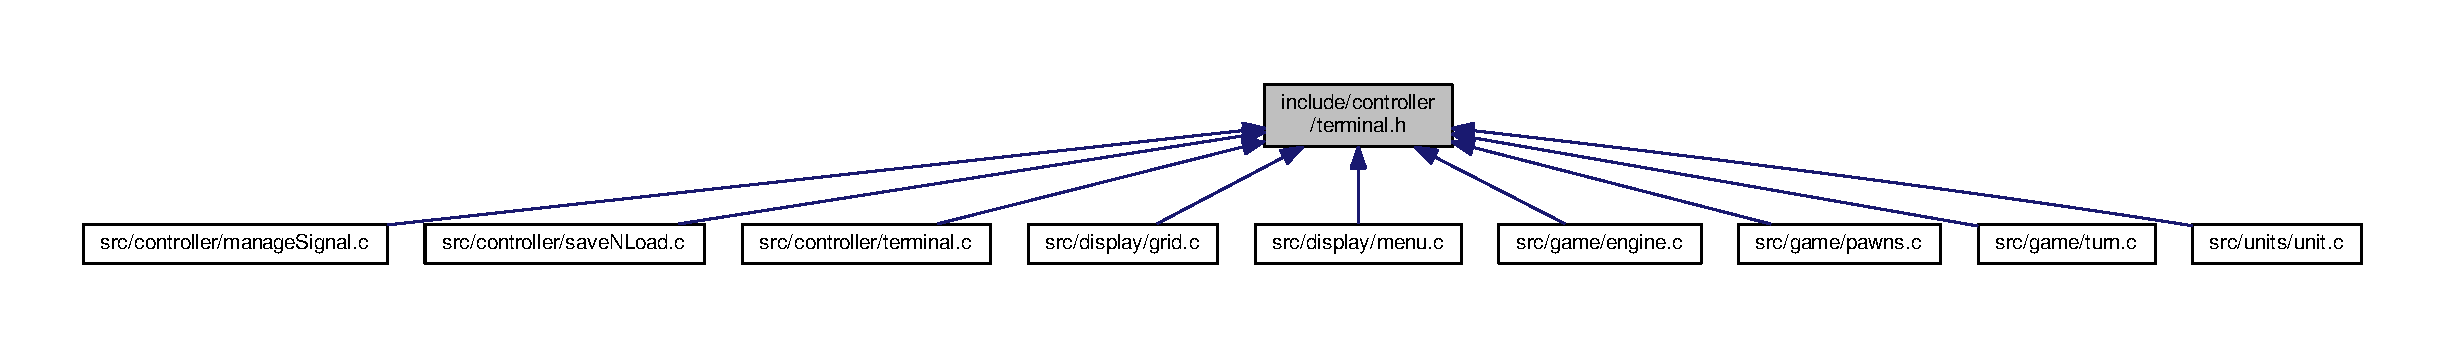
\includegraphics[width=350pt]{terminal_8h__dep__incl}
\end{center}
\end{figure}
\subsection*{Énumérations}
\begin{DoxyCompactItemize}
\item 
\hypertarget{terminal_8h_ac8946d2a0583792b5f43ba0f6616ff84}{}enum \hyperlink{terminal_8h_ac8946d2a0583792b5f43ba0f6616ff84}{terminal} \{ \\*
{\bfseries black}, 
{\bfseries red}, 
{\bfseries green}, 
{\bfseries yellow}, 
\\*
{\bfseries blue}, 
{\bfseries magenta}, 
{\bfseries cyan}, 
{\bfseries white}
 \}\label{terminal_8h_ac8946d2a0583792b5f43ba0f6616ff84}

\begin{DoxyCompactList}\small\item\em \hyperlink{terminal_8h}{terminal.\+h} \end{DoxyCompactList}\item 
\hypertarget{terminal_8h_a72bba37476e63c27f023823f17619987}{}enum \hyperlink{terminal_8h_a72bba37476e63c27f023823f17619987}{screen} \{ {\bfseries reinit} = 0, 
{\bfseries blink} = 5, 
{\bfseries invert\+Color} = 7
 \}\label{terminal_8h_a72bba37476e63c27f023823f17619987}

\begin{DoxyCompactList}\small\item\em \hyperlink{terminal_8h}{terminal.\+h} \end{DoxyCompactList}\end{DoxyCompactItemize}
\subsection*{Fonctions}
\begin{DoxyCompactItemize}
\item 
void \hyperlink{terminal_8h_aa1b198e2a86cf333bd2b8d74e21409f1}{color} (int color, char type\mbox{[}$\,$\mbox{]})
\begin{DoxyCompactList}\small\item\em Met en couleurs le texte ou l\textquotesingle{}écran. \end{DoxyCompactList}\item 
void \hyperlink{terminal_8h_a728c5deabcb9e271c6962577c60ef566}{font\+Color} (int \hyperlink{terminal_8h_aa1b198e2a86cf333bd2b8d74e21409f1}{color})
\begin{DoxyCompactList}\small\item\em Met en couleurs la police. \end{DoxyCompactList}\item 
\hypertarget{terminal_8h_a9d7e8af417b6d543da691e9c0e2f6f9f}{}void \hyperlink{terminal_8h_a9d7e8af417b6d543da691e9c0e2f6f9f}{clear\+Screen} ()\label{terminal_8h_a9d7e8af417b6d543da691e9c0e2f6f9f}

\begin{DoxyCompactList}\small\item\em Efface l\textquotesingle{}écran. \end{DoxyCompactList}\item 
void \hyperlink{terminal_8h_aafe20dae78dfbeea7c9102fadcfba1e0}{reinit\+Color} ()
\begin{DoxyCompactList}\small\item\em Réinitialise les couleurs. \end{DoxyCompactList}\end{DoxyCompactItemize}


\subsection{Description détaillée}
En-\/tête gestion du terminal. 

\begin{DoxyAuthor}{Auteur}
Cousin Brandon Chaudemanche Ewen Biardeau Tristan 
\end{DoxyAuthor}
\begin{DoxyVersion}{Version}
v1.\+00 
\end{DoxyVersion}
\begin{DoxyDate}{Date}
18/12/2015 
\end{DoxyDate}


\subsection{Documentation des fonctions}
\hypertarget{terminal_8h_aa1b198e2a86cf333bd2b8d74e21409f1}{}\index{terminal.\+h@{terminal.\+h}!color@{color}}
\index{color@{color}!terminal.\+h@{terminal.\+h}}
\subsubsection[{color}]{\setlength{\rightskip}{0pt plus 5cm}void color (
\begin{DoxyParamCaption}
\item[{int}]{color, }
\item[{char}]{type\mbox{[}$\,$\mbox{]}}
\end{DoxyParamCaption}
)}\label{terminal_8h_aa1b198e2a86cf333bd2b8d74e21409f1}


Met en couleurs le texte ou l\textquotesingle{}écran. 

Met en couleurs le texte ou l\textquotesingle{}écran.


\begin{DoxyParams}{Paramètres}
{\em color} & Couleur à utiliser \\
\hline
{\em type} & Texte à changer de couleur ou arrière plan \\
\hline
\end{DoxyParams}


Définition à la ligne 51 du fichier terminal.\+c.

\hypertarget{terminal_8h_a728c5deabcb9e271c6962577c60ef566}{}\index{terminal.\+h@{terminal.\+h}!font\+Color@{font\+Color}}
\index{font\+Color@{font\+Color}!terminal.\+h@{terminal.\+h}}
\subsubsection[{font\+Color}]{\setlength{\rightskip}{0pt plus 5cm}void font\+Color (
\begin{DoxyParamCaption}
\item[{int}]{color}
\end{DoxyParamCaption}
)}\label{terminal_8h_a728c5deabcb9e271c6962577c60ef566}


Met en couleurs la police. 

Met en couleurs la police.


\begin{DoxyParams}{Paramètres}
{\em color} & Couleur à utiliser \\
\hline
\end{DoxyParams}


Définition à la ligne 76 du fichier terminal.\+c.

\hypertarget{terminal_8h_aafe20dae78dfbeea7c9102fadcfba1e0}{}\index{terminal.\+h@{terminal.\+h}!reinit\+Color@{reinit\+Color}}
\index{reinit\+Color@{reinit\+Color}!terminal.\+h@{terminal.\+h}}
\subsubsection[{reinit\+Color}]{\setlength{\rightskip}{0pt plus 5cm}void reinit\+Color (
\begin{DoxyParamCaption}
{}
\end{DoxyParamCaption}
)}\label{terminal_8h_aafe20dae78dfbeea7c9102fadcfba1e0}


Réinitialise les couleurs. 

Réinitialise les couleurs. 

Définition à la ligne 67 du fichier terminal.\+c.


\hypertarget{grid_8h}{}\section{Référence du fichier include/display/grid.h}
\label{grid_8h}\index{include/display/grid.\+h@{include/display/grid.\+h}}


En-\/tête gestion de la grille.  


Ce graphe montre quels fichiers incluent directement ou indirectement ce fichier \+:\nopagebreak
\begin{figure}[H]
\begin{center}
\leavevmode
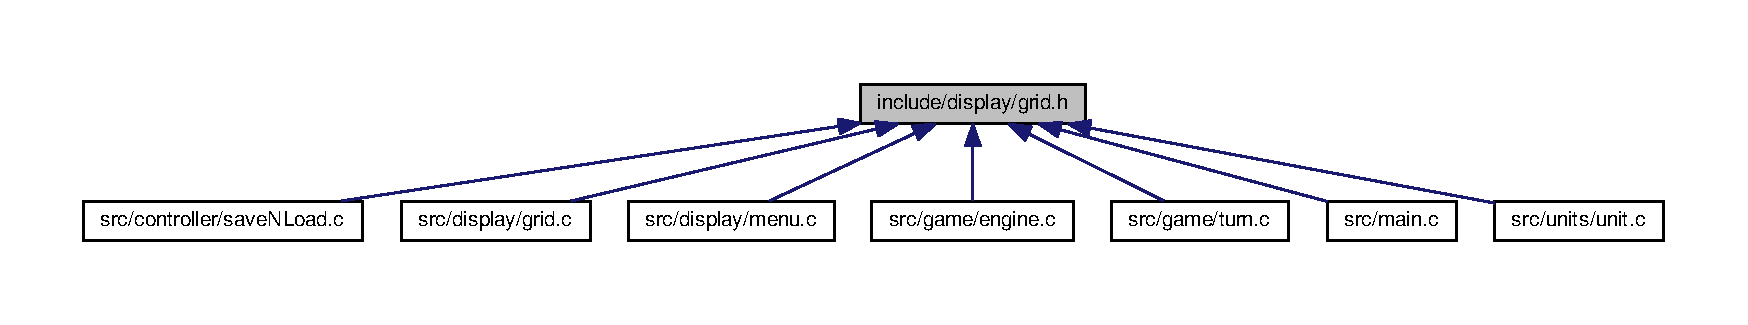
\includegraphics[width=350pt]{grid_8h__dep__incl}
\end{center}
\end{figure}
\subsection*{Macros}
\begin{DoxyCompactItemize}
\item 
\hypertarget{grid_8h_a171160a766f85c8816b898ed24d28408}{}\#define \hyperlink{grid_8h_a171160a766f85c8816b898ed24d28408}{R\+B}~\char`\"{}\textbackslash{}e(0\textbackslash{}x6a\textbackslash{}e(B\char`\"{}\label{grid_8h_a171160a766f85c8816b898ed24d28408}

\begin{DoxyCompactList}\small\item\em 188 Right Bottom corner \end{DoxyCompactList}\item 
\hypertarget{grid_8h_ad05d2f1b67cda860903cecd9f21b6b9f}{}\#define \hyperlink{grid_8h_ad05d2f1b67cda860903cecd9f21b6b9f}{R\+T}~\char`\"{}\textbackslash{}e(0\textbackslash{}x6b\textbackslash{}e(B\char`\"{}\label{grid_8h_ad05d2f1b67cda860903cecd9f21b6b9f}

\begin{DoxyCompactList}\small\item\em 187 Right Top corner \end{DoxyCompactList}\item 
\hypertarget{grid_8h_aaf56b99cbe34023f42ce5b7878c827d8}{}\#define \hyperlink{grid_8h_aaf56b99cbe34023f42ce5b7878c827d8}{L\+T}~\char`\"{}\textbackslash{}e(0\textbackslash{}x6c\textbackslash{}e(B\char`\"{}\label{grid_8h_aaf56b99cbe34023f42ce5b7878c827d8}

\begin{DoxyCompactList}\small\item\em 201 Left Top cornet \end{DoxyCompactList}\item 
\hypertarget{grid_8h_acc55daa58d88a3612f2ef74a6abbe97f}{}\#define \hyperlink{grid_8h_acc55daa58d88a3612f2ef74a6abbe97f}{L\+B}~\char`\"{}\textbackslash{}e(0\textbackslash{}x6d\textbackslash{}e(B\char`\"{}\label{grid_8h_acc55daa58d88a3612f2ef74a6abbe97f}

\begin{DoxyCompactList}\small\item\em 200 Left Bottom corner \end{DoxyCompactList}\item 
\hypertarget{grid_8h_af66e7c3d47aab0745e29e697ea13c6f6}{}\#define \hyperlink{grid_8h_af66e7c3d47aab0745e29e697ea13c6f6}{V\+L}~\char`\"{}\textbackslash{}e(0\textbackslash{}x78\textbackslash{}e(B\char`\"{}\label{grid_8h_af66e7c3d47aab0745e29e697ea13c6f6}

\begin{DoxyCompactList}\small\item\em 186 Vertical Line \end{DoxyCompactList}\item 
\hypertarget{grid_8h_a1592226003ffbf8fa1b036eae180b6f5}{}\#define \hyperlink{grid_8h_a1592226003ffbf8fa1b036eae180b6f5}{H\+L}~\char`\"{}\textbackslash{}e(0\textbackslash{}x71\textbackslash{}e(B\char`\"{}\label{grid_8h_a1592226003ffbf8fa1b036eae180b6f5}

\begin{DoxyCompactList}\small\item\em 205 Horizontal Line \end{DoxyCompactList}\end{DoxyCompactItemize}
\subsection*{Fonctions}
\begin{DoxyCompactItemize}
\item 
void \hyperlink{grid_8h_aad3077ff809cfe68afdb06ef3aa5497f}{grid\+Disp} ()
\begin{DoxyCompactList}\small\item\em Affiche la grille. \end{DoxyCompactList}\end{DoxyCompactItemize}


\subsection{Description détaillée}
En-\/tête gestion de la grille. 

\begin{DoxyAuthor}{Auteur}
Cousin Brandon Chaudemanche Ewen Biardeau Tristan 
\end{DoxyAuthor}
\begin{DoxyVersion}{Version}
v1.\+00 
\end{DoxyVersion}
\begin{DoxyDate}{Date}
18/12/2015 
\end{DoxyDate}


\subsection{Documentation des fonctions}
\hypertarget{grid_8h_aad3077ff809cfe68afdb06ef3aa5497f}{}\index{grid.\+h@{grid.\+h}!grid\+Disp@{grid\+Disp}}
\index{grid\+Disp@{grid\+Disp}!grid.\+h@{grid.\+h}}
\subsubsection[{grid\+Disp}]{\setlength{\rightskip}{0pt plus 5cm}void grid\+Disp (
\begin{DoxyParamCaption}
{}
\end{DoxyParamCaption}
)}\label{grid_8h_aad3077ff809cfe68afdb06ef3aa5497f}


Affiche la grille. 

Affiche la grille. 

Définition à la ligne 78 du fichier grid.\+c.


\hypertarget{menu_8h}{}\section{Référence du fichier include/display/menu.h}
\label{menu_8h}\index{include/display/menu.\+h@{include/display/menu.\+h}}


En-\/tête gestion des menus.  


Ce graphe montre quels fichiers incluent directement ou indirectement ce fichier \+:\nopagebreak
\begin{figure}[H]
\begin{center}
\leavevmode
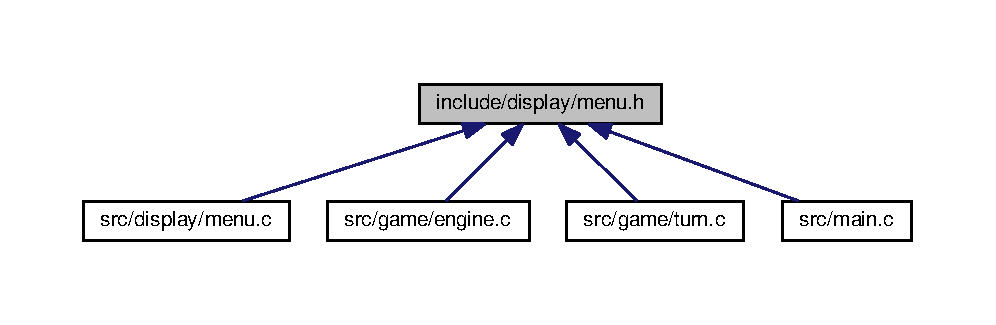
\includegraphics[width=350pt]{menu_8h__dep__incl}
\end{center}
\end{figure}
\subsection*{Fonctions}
\begin{DoxyCompactItemize}
\item 
void \hyperlink{menu_8h_ab3002fe8e0074c9e2ecb5b835e5e819f}{main\+Menu} ()
\begin{DoxyCompactList}\small\item\em Menu principal. \end{DoxyCompactList}\item 
void \hyperlink{menu_8h_ac722505df6f214afc5d28c922da5e0c7}{game\+Menu} ()
\begin{DoxyCompactList}\small\item\em Menu de jeu. \end{DoxyCompactList}\item 
void \hyperlink{menu_8h_a4e88525c8d42c1affc4e8ef8e7ebca44}{unit\+Menu} (int choice)
\begin{DoxyCompactList}\small\item\em Menu de sélection de l\textquotesingle{}unité \end{DoxyCompactList}\item 
void \hyperlink{menu_8h_a2eb7eed865e161dfaf02136f6c22e873}{unit\+List} ()
\begin{DoxyCompactList}\small\item\em Listes des unités du jeu. \end{DoxyCompactList}\item 
\hypertarget{menu_8h_a57c1286e99f7c479a937ebbafcfe8681}{}void \hyperlink{menu_8h_a57c1286e99f7c479a937ebbafcfe8681}{main\+Help} ()\label{menu_8h_a57c1286e99f7c479a937ebbafcfe8681}

\begin{DoxyCompactList}\small\item\em Menu d\textquotesingle{}aide principal. \end{DoxyCompactList}\item 
void \hyperlink{menu_8h_aea4bcea967e5f0d7bb00517649f21701}{help\+Unit} ()
\begin{DoxyCompactList}\small\item\em Menu d\textquotesingle{}aide des unités. \end{DoxyCompactList}\item 
void \hyperlink{menu_8h_aac6cc2265bfc1481caf987f92bece27b}{disp\+Direction} ()
\begin{DoxyCompactList}\small\item\em Affiche la liste des directions. \end{DoxyCompactList}\end{DoxyCompactItemize}


\subsection{Description détaillée}
En-\/tête gestion des menus. 

\begin{DoxyAuthor}{Auteur}
Cousin Brandon Chaudemanche Ewen Biardeau Tristan 
\end{DoxyAuthor}
\begin{DoxyVersion}{Version}
v1.\+00 
\end{DoxyVersion}
\begin{DoxyDate}{Date}
18/12/2015 
\end{DoxyDate}


\subsection{Documentation des fonctions}
\hypertarget{menu_8h_aac6cc2265bfc1481caf987f92bece27b}{}\index{menu.\+h@{menu.\+h}!disp\+Direction@{disp\+Direction}}
\index{disp\+Direction@{disp\+Direction}!menu.\+h@{menu.\+h}}
\subsubsection[{disp\+Direction}]{\setlength{\rightskip}{0pt plus 5cm}void disp\+Direction (
\begin{DoxyParamCaption}
{}
\end{DoxyParamCaption}
)}\label{menu_8h_aac6cc2265bfc1481caf987f92bece27b}


Affiche la liste des directions. 

Affiche la liste des directions. 

Définition à la ligne 458 du fichier menu.\+c.

\hypertarget{menu_8h_ac722505df6f214afc5d28c922da5e0c7}{}\index{menu.\+h@{menu.\+h}!game\+Menu@{game\+Menu}}
\index{game\+Menu@{game\+Menu}!menu.\+h@{menu.\+h}}
\subsubsection[{game\+Menu}]{\setlength{\rightskip}{0pt plus 5cm}void game\+Menu (
\begin{DoxyParamCaption}
{}
\end{DoxyParamCaption}
)}\label{menu_8h_ac722505df6f214afc5d28c922da5e0c7}


Menu de jeu. 

Menu de jeu. 

Définition à la ligne 470 du fichier menu.\+c.

\hypertarget{menu_8h_aea4bcea967e5f0d7bb00517649f21701}{}\index{menu.\+h@{menu.\+h}!help\+Unit@{help\+Unit}}
\index{help\+Unit@{help\+Unit}!menu.\+h@{menu.\+h}}
\subsubsection[{help\+Unit}]{\setlength{\rightskip}{0pt plus 5cm}void help\+Unit (
\begin{DoxyParamCaption}
{}
\end{DoxyParamCaption}
)}\label{menu_8h_aea4bcea967e5f0d7bb00517649f21701}


Menu d\textquotesingle{}aide des unités. 

Menu d\textquotesingle{}aide des unités. 

Définition à la ligne 222 du fichier menu.\+c.

\hypertarget{menu_8h_ab3002fe8e0074c9e2ecb5b835e5e819f}{}\index{menu.\+h@{menu.\+h}!main\+Menu@{main\+Menu}}
\index{main\+Menu@{main\+Menu}!menu.\+h@{menu.\+h}}
\subsubsection[{main\+Menu}]{\setlength{\rightskip}{0pt plus 5cm}void main\+Menu (
\begin{DoxyParamCaption}
{}
\end{DoxyParamCaption}
)}\label{menu_8h_ab3002fe8e0074c9e2ecb5b835e5e819f}


Menu principal. 

Menu principal. 

Définition à la ligne 24 du fichier menu.\+c.

\hypertarget{menu_8h_a2eb7eed865e161dfaf02136f6c22e873}{}\index{menu.\+h@{menu.\+h}!unit\+List@{unit\+List}}
\index{unit\+List@{unit\+List}!menu.\+h@{menu.\+h}}
\subsubsection[{unit\+List}]{\setlength{\rightskip}{0pt plus 5cm}void unit\+List (
\begin{DoxyParamCaption}
{}
\end{DoxyParamCaption}
)}\label{menu_8h_a2eb7eed865e161dfaf02136f6c22e873}


Listes des unités du jeu. 

Listes des unités du jeu. 

Définition à la ligne 593 du fichier menu.\+c.

\hypertarget{menu_8h_a4e88525c8d42c1affc4e8ef8e7ebca44}{}\index{menu.\+h@{menu.\+h}!unit\+Menu@{unit\+Menu}}
\index{unit\+Menu@{unit\+Menu}!menu.\+h@{menu.\+h}}
\subsubsection[{unit\+Menu}]{\setlength{\rightskip}{0pt plus 5cm}void unit\+Menu (
\begin{DoxyParamCaption}
\item[{int}]{choice}
\end{DoxyParamCaption}
)}\label{menu_8h_a4e88525c8d42c1affc4e8ef8e7ebca44}


Menu de sélection de l\textquotesingle{}unité 


\begin{DoxyParams}{Paramètres}
{\em choice} & Choix de l\textquotesingle{}action pour l\textquotesingle{}unité \\
\hline
\end{DoxyParams}


Définition à la ligne 517 du fichier menu.\+c.


\hypertarget{engine_8h}{}\section{Référence du fichier include/game/engine.h}
\label{engine_8h}\index{include/game/engine.\+h@{include/game/engine.\+h}}


En-\/tête moteur de jeu.  


{\ttfamily \#include $<$stdbool.\+h$>$}\\*
{\ttfamily \#include $<$string.\+h$>$}\\*
{\ttfamily \#include $<$stdlib.\+h$>$}\\*
Graphe des dépendances par inclusion de engine.\+h\+:\nopagebreak
\begin{figure}[H]
\begin{center}
\leavevmode
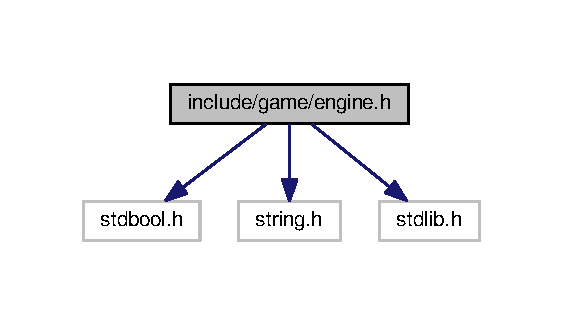
\includegraphics[width=270pt]{engine_8h__incl}
\end{center}
\end{figure}
Ce graphe montre quels fichiers incluent directement ou indirectement ce fichier \+:\nopagebreak
\begin{figure}[H]
\begin{center}
\leavevmode
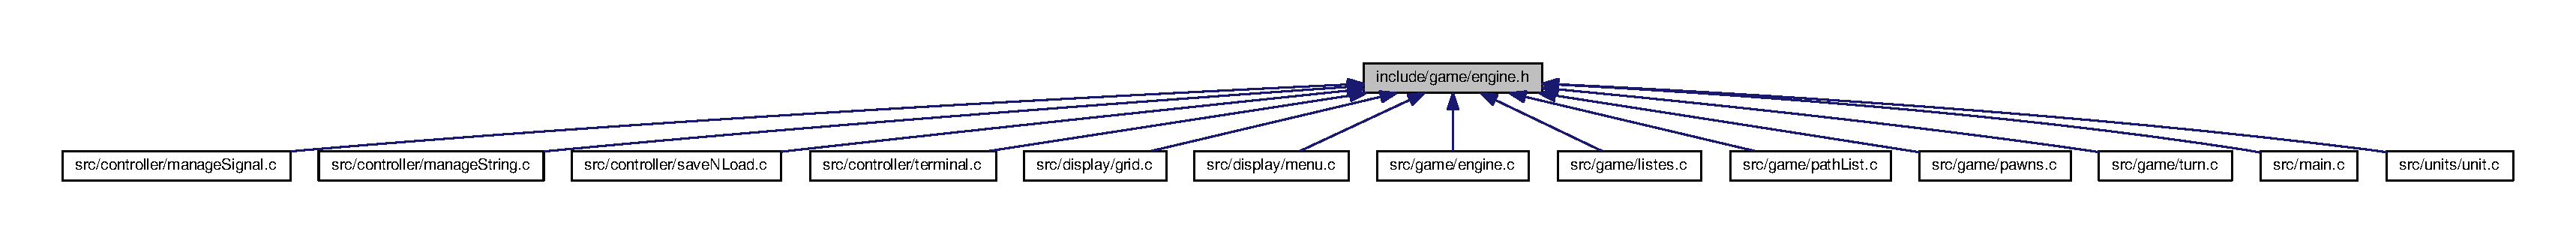
\includegraphics[width=350pt]{engine_8h__dep__incl}
\end{center}
\end{figure}
\subsection*{Classes}
\begin{DoxyCompactItemize}
\item 
struct \hyperlink{structtargetStat}{target\+Stat}
\begin{DoxyCompactList}\small\item\em Représente les informations liées aux cibles. \end{DoxyCompactList}\item 
struct \hyperlink{structunitStat}{unit\+Stat}
\begin{DoxyCompactList}\small\item\em Représente les statistiques d\textquotesingle{}une unité \end{DoxyCompactList}\item 
struct \hyperlink{structvector}{vector}
\begin{DoxyCompactList}\small\item\em Représente les coordonnées d\textquotesingle{}un vecteur. \end{DoxyCompactList}\item 
struct \hyperlink{structunit}{unit}
\begin{DoxyCompactList}\small\item\em Représente une unité \end{DoxyCompactList}\end{DoxyCompactItemize}
\subsection*{Macros}
\begin{DoxyCompactItemize}
\item 
\hypertarget{engine_8h_a0240ac851181b84ac374872dc5434ee4}{}\#define \hyperlink{engine_8h_a0240ac851181b84ac374872dc5434ee4}{N}~11\label{engine_8h_a0240ac851181b84ac374872dc5434ee4}

\begin{DoxyCompactList}\small\item\em Taille de la grille. \end{DoxyCompactList}\item 
\hypertarget{engine_8h_afb66c371fb21dd91933e5f45ff4ce817}{}\#define \hyperlink{engine_8h_afb66c371fb21dd91933e5f45ff4ce817}{N\+B\+\_\+\+L\+I\+S\+T\+S\+\_\+\+E\+N\+G\+I\+N\+E}~2\label{engine_8h_afb66c371fb21dd91933e5f45ff4ce817}

\begin{DoxyCompactList}\small\item\em Nombre de liste additionnelles nécessaires pour le jeu. \end{DoxyCompactList}\item 
\hypertarget{engine_8h_a063165e36f1905a19e98c412ee181878}{}\#define \hyperlink{engine_8h_a063165e36f1905a19e98c412ee181878}{N\+B\+\_\+\+P\+L\+A\+Y\+E\+R\+S}~2\label{engine_8h_a063165e36f1905a19e98c412ee181878}

\begin{DoxyCompactList}\small\item\em Nombre de joueurs. \end{DoxyCompactList}\item 
\hypertarget{engine_8h_ac4bf44d5b138de69050557acc46b4700}{}\#define \hyperlink{engine_8h_ac4bf44d5b138de69050557acc46b4700}{N\+B\+\_\+\+L\+I\+N\+E\+S}~3\label{engine_8h_ac4bf44d5b138de69050557acc46b4700}

\begin{DoxyCompactList}\small\item\em Limite du camp du joueur. \end{DoxyCompactList}\item 
\hypertarget{engine_8h_a5165d4965ab32e87f1dd3181a41f0a7a}{}\#define \hyperlink{engine_8h_a5165d4965ab32e87f1dd3181a41f0a7a}{N\+B\+\_\+\+U\+N\+I\+T\+S}~21\label{engine_8h_a5165d4965ab32e87f1dd3181a41f0a7a}

\begin{DoxyCompactList}\small\item\em Nombre d\textquotesingle{}unités dans le jeu. \end{DoxyCompactList}\item 
\hypertarget{engine_8h_a21db47461d910a7cad180b5532f1a7f8}{}\#define \hyperlink{engine_8h_a21db47461d910a7cad180b5532f1a7f8}{N\+B\+\_\+\+M\+A\+X\+\_\+\+E\+F\+F\+E\+C\+T}~6\label{engine_8h_a21db47461d910a7cad180b5532f1a7f8}

\begin{DoxyCompactList}\small\item\em Nombre total de status différent. \end{DoxyCompactList}\item 
\hypertarget{engine_8h_a26f6ab8604048e4b80c8bc535ff4bad9}{}\#define \hyperlink{engine_8h_a26f6ab8604048e4b80c8bc535ff4bad9}{M\+A\+N\+D\+A\+T\+O\+R\+Y\+\_\+\+S\+T\+A\+T\+S}~12\label{engine_8h_a26f6ab8604048e4b80c8bc535ff4bad9}

\begin{DoxyCompactList}\small\item\em Nombre de stats obligatoire. \end{DoxyCompactList}\item 
\hypertarget{engine_8h_a89f0201fca94cbc3ca0f5fbce851e7c9}{}\#define \hyperlink{engine_8h_a89f0201fca94cbc3ca0f5fbce851e7c9}{F\+I\+R\+S\+T\+\_\+\+P\+L\+A\+Y\+E\+R}~0\label{engine_8h_a89f0201fca94cbc3ca0f5fbce851e7c9}

\begin{DoxyCompactList}\small\item\em Définis la valeur du premier joueur. \end{DoxyCompactList}\item 
\hypertarget{engine_8h_a2aaa949daff5a729be2acff95b7d0fed}{}\#define \hyperlink{engine_8h_a2aaa949daff5a729be2acff95b7d0fed}{N\+B\+\_\+\+M\+A\+X\+\_\+\+K\+N}~3\label{engine_8h_a2aaa949daff5a729be2acff95b7d0fed}

\begin{DoxyCompactList}\small\item\em Nombre max de Guerrier par joueur. \end{DoxyCompactList}\item 
\hypertarget{engine_8h_add7fd7b19c17c1ac0918a95089e2c7f9}{}\#define \hyperlink{engine_8h_add7fd7b19c17c1ac0918a95089e2c7f9}{N\+B\+\_\+\+M\+A\+X\+\_\+\+S\+C}~2\label{engine_8h_add7fd7b19c17c1ac0918a95089e2c7f9}

\begin{DoxyCompactList}\small\item\em Nombre max de Recrue par joueur. \end{DoxyCompactList}\item 
\hypertarget{engine_8h_a3e866793438e4da9a36962a808d664d7}{}\#define \hyperlink{engine_8h_a3e866793438e4da9a36962a808d664d7}{N\+B\+\_\+\+M\+A\+X\+\_\+\+S\+G}~2\label{engine_8h_a3e866793438e4da9a36962a808d664d7}

\begin{DoxyCompactList}\small\item\em Nombre max de Golem de pierre par joueur. \end{DoxyCompactList}\item 
\hypertarget{engine_8h_a0838a4817c4beea8be5cab65cad54122}{}\#define \hyperlink{engine_8h_a0838a4817c4beea8be5cab65cad54122}{N\+B\+\_\+\+M\+A\+X\+\_\+\+L\+T}~1\label{engine_8h_a0838a4817c4beea8be5cab65cad54122}

\begin{DoxyCompactList}\small\item\em Nombre max de Lightning totem par joueur. \end{DoxyCompactList}\item 
\hypertarget{engine_8h_aacfee0d79acf9b6378182a8aa2ee0226}{}\#define \hyperlink{engine_8h_aacfee0d79acf9b6378182a8aa2ee0226}{N\+B\+\_\+\+M\+A\+X\+\_\+\+D\+R}~2\label{engine_8h_aacfee0d79acf9b6378182a8aa2ee0226}

\begin{DoxyCompactList}\small\item\em Nombre max de Dragon par joueur. \end{DoxyCompactList}\item 
\hypertarget{engine_8h_a4d20c3d53297ab3184e441f7a85df250}{}\#define \hyperlink{engine_8h_a4d20c3d53297ab3184e441f7a85df250}{N\+B\+\_\+\+M\+A\+X\+\_\+\+F\+U}~2\label{engine_8h_a4d20c3d53297ab3184e441f7a85df250}

\begin{DoxyCompactList}\small\item\em Nombre max de Furgon par joueur. \end{DoxyCompactList}\item 
\hypertarget{engine_8h_aef5bbc6c16b0afbb41c6f723b099e599}{}\#define \hyperlink{engine_8h_aef5bbc6c16b0afbb41c6f723b099e599}{N\+B\+\_\+\+M\+A\+X\+\_\+\+U\+N\+I\+T}~5\label{engine_8h_aef5bbc6c16b0afbb41c6f723b099e599}

\begin{DoxyCompactList}\small\item\em Nombre max d\textquotesingle{}unité par joueur. \end{DoxyCompactList}\item 
\hypertarget{engine_8h_a207089a6eadde7204cda31d055e4d3a1}{}\#define \hyperlink{engine_8h_a207089a6eadde7204cda31d055e4d3a1}{N\+B\+\_\+\+M\+A\+X\+\_\+\+D\+E\+C\+O\+R}~7\label{engine_8h_a207089a6eadde7204cda31d055e4d3a1}

\begin{DoxyCompactList}\small\item\em Nombre max de décor. \end{DoxyCompactList}\end{DoxyCompactItemize}
\subsection*{Énumérations}
\begin{DoxyCompactItemize}
\item 
\hypertarget{engine_8h_a468af3d7606639780e81c5e1e403b356}{}enum \hyperlink{engine_8h_a468af3d7606639780e81c5e1e403b356}{cardinal} \{ {\bfseries north}, 
{\bfseries east}, 
{\bfseries south}, 
{\bfseries west}
 \}\label{engine_8h_a468af3d7606639780e81c5e1e403b356}

\begin{DoxyCompactList}\small\item\em \hyperlink{engine_8h}{engine.\+h} \end{DoxyCompactList}\item 
\hypertarget{engine_8h_af7667555c2dcfbdd55ec3e9dd6a907ba}{}enum \hyperlink{engine_8h_af7667555c2dcfbdd55ec3e9dd6a907ba}{unit\+Name} \{ \\*
{\bfseries empty}, 
{\bfseries decors}, 
{\bfseries knight}, 
{\bfseries scout}, 
\\*
{\bfseries assassin}, 
{\bfseries cleric}, 
{\bfseries pyromancer}, 
{\bfseries enchantress}, 
\\*
{\bfseries dragonborn}, 
{\bfseries dark\+Witch}, 
{\bfseries lightning\+Totem}, 
{\bfseries barrier\+Totem}, 
\\*
{\bfseries mud\+Golem}, 
{\bfseries golem\+Ambusher}, 
{\bfseries frost\+Golem}, 
{\bfseries stone\+Golem}, 
\\*
{\bfseries dragon\+Tyrant}, 
{\bfseries berserker}, 
{\bfseries beast\+Rider}, 
{\bfseries poison\+Wisp}, 
\\*
{\bfseries furgon}
 \}\label{engine_8h_af7667555c2dcfbdd55ec3e9dd6a907ba}

\begin{DoxyCompactList}\small\item\em \hyperlink{engine_8h}{engine.\+h} \end{DoxyCompactList}\item 
\hypertarget{engine_8h_ac5ece9b6993cd3565502866b56317e84}{}enum \hyperlink{engine_8h_ac5ece9b6993cd3565502866b56317e84}{unit\+Effect} \{ \\*
{\bfseries none}, 
{\bfseries P\+O\+W\+E\+R\+\_\+\+B\+O\+N\+U\+S}, 
{\bfseries A\+R\+M\+O\+R\+\_\+\+B\+O\+N\+U\+S}, 
{\bfseries B\+A\+R\+R\+I\+E\+R}, 
\\*
{\bfseries P\+O\+I\+S\+O\+N}, 
{\bfseries P\+A\+R\+A\+L\+Y\+S\+E}, 
{\bfseries F\+O\+C\+U\+S}
 \}\label{engine_8h_ac5ece9b6993cd3565502866b56317e84}

\begin{DoxyCompactList}\small\item\em \hyperlink{engine_8h}{engine.\+h} \end{DoxyCompactList}\end{DoxyCompactItemize}
\subsection*{Fonctions}
\begin{DoxyCompactItemize}
\item 
bool \hyperlink{engine_8h_a3ee2a4066924757ade5530e7041a2ad1}{is\+Surrounded} (\hyperlink{structvector}{vector} current\+Unit)
\begin{DoxyCompactList}\small\item\em Vérifie si une unité est entourée. \end{DoxyCompactList}\item 
void \hyperlink{engine_8h_a43ae9a7f0ac55585ed6375c580abcaf0}{game\+Init} ()
\begin{DoxyCompactList}\small\item\em Initialise le jeu. \end{DoxyCompactList}\item 
bool \hyperlink{engine_8h_acd459b9ed1aaf8c05cdd3887e86b8668}{select\+Unit} (\hyperlink{structvector}{vector} $\ast$coord\+Unit)
\begin{DoxyCompactList}\small\item\em Sélectionne une unité \end{DoxyCompactList}\item 
void \hyperlink{engine_8h_a7de2811c781a1136844609cc95e26464}{set\+Target} (\hyperlink{engine_8h_af7667555c2dcfbdd55ec3e9dd6a907ba}{unit\+Name} name, \hyperlink{structvector}{vector} coord\+Unit, int color\+Disp)
\begin{DoxyCompactList}\small\item\em Définis les cibles. \end{DoxyCompactList}\item 
void \hyperlink{engine_8h_a42359e6294ac21935ecc2d77140da492}{launch\+Attack} (\hyperlink{structvector}{vector} coord\+Source, \hyperlink{structvector}{vector} coord\+Target)
\begin{DoxyCompactList}\small\item\em Lance une attaque. \end{DoxyCompactList}\item 
void \hyperlink{engine_8h_a8aca0579aac39cc7e3c41342d89fe1b7}{movable} (int color\+Disp)
\begin{DoxyCompactList}\small\item\em Fait la liste des unités déplaçables. \end{DoxyCompactList}\item 
void \hyperlink{engine_8h_ae40e16d551936cea056a982196273bde}{attackable} (int color\+Disp)
\begin{DoxyCompactList}\small\item\em Fait la liste des unités pouvant attaquer. \end{DoxyCompactList}\item 
void \hyperlink{engine_8h_a309311c2d6a59c5998007d0e5f215d4d}{tile\+Walkable} (\hyperlink{structvector}{vector} coord\+Unit, int color\+Disp)
\begin{DoxyCompactList}\small\item\em Fait la liste des cases atteignables par l\textquotesingle{}unité \end{DoxyCompactList}\item 
bool \hyperlink{engine_8h_a548c013433afab60c17fd9950fb7248f}{possible\+Path} (\hyperlink{structvector}{vector} coord\+Unit)
\begin{DoxyCompactList}\small\item\em Vérifie qu\textquotesingle{}un chemin est possible. \end{DoxyCompactList}\item 
bool \hyperlink{engine_8h_ad0311428b7054a1ab271d3a433316704}{path\+Find} (\hyperlink{structvector}{vector}, \hyperlink{structvector}{vector})
\begin{DoxyCompactList}\small\item\em Trouve une chemin vers la destination. \end{DoxyCompactList}\item 
\hypertarget{engine_8h_ab1f321a2f17fa8ba0f5ab4e2621fd6d6}{}void \hyperlink{engine_8h_ab1f321a2f17fa8ba0f5ab4e2621fd6d6}{start\+Game} ()\label{engine_8h_ab1f321a2f17fa8ba0f5ab4e2621fd6d6}

\begin{DoxyCompactList}\small\item\em Débute la partie. \end{DoxyCompactList}\item 
void \hyperlink{engine_8h_ac98554d7cf4b7b0000029fac97218be4}{line\+Of\+Sight} (\hyperlink{structvector}{vector}, \hyperlink{structvector}{vector})
\begin{DoxyCompactList}\small\item\em Ligne de vue de l\textquotesingle{}archer. \end{DoxyCompactList}\end{DoxyCompactItemize}
\subsection*{Variables}
\begin{DoxyCompactItemize}
\item 
\hyperlink{structunit}{unit} \hyperlink{engine_8h_a5987e3369c71f1edb157786e4c75875b}{grid} \mbox{[}\hyperlink{engine_8h_a0240ac851181b84ac374872dc5434ee4}{N}\mbox{]}\mbox{[}\hyperlink{engine_8h_a0240ac851181b84ac374872dc5434ee4}{N}\mbox{]}
\begin{DoxyCompactList}\small\item\em Représentation d\textquotesingle{}une grille d\textquotesingle{}unité globale. \end{DoxyCompactList}\item 
int \hyperlink{engine_8h_afaa2c64a9fd09c382394b57006c470ce}{no\+Player}
\begin{DoxyCompactList}\small\item\em Représentation du joueur. \end{DoxyCompactList}\end{DoxyCompactItemize}


\subsection{Description détaillée}
En-\/tête moteur de jeu. 

\begin{DoxyAuthor}{Auteur}
Cousin Brandon Chaudemanche Ewen Biardeau Tristan 
\end{DoxyAuthor}
\begin{DoxyVersion}{Version}
v1.\+00 
\end{DoxyVersion}
\begin{DoxyDate}{Date}
18/12/2015 
\end{DoxyDate}


\subsection{Documentation des fonctions}
\hypertarget{engine_8h_ae40e16d551936cea056a982196273bde}{}\index{engine.\+h@{engine.\+h}!attackable@{attackable}}
\index{attackable@{attackable}!engine.\+h@{engine.\+h}}
\subsubsection[{attackable}]{\setlength{\rightskip}{0pt plus 5cm}void attackable (
\begin{DoxyParamCaption}
\item[{int}]{color\+Disp}
\end{DoxyParamCaption}
)}\label{engine_8h_ae40e16d551936cea056a982196273bde}


Fait la liste des unités pouvant attaquer. 


\begin{DoxyParams}{Paramètres}
{\em color\+Disp} & Couleur d\textquotesingle{}affichage \\
\hline
\end{DoxyParams}


Définition à la ligne 164 du fichier engine.\+c.

\hypertarget{engine_8h_a43ae9a7f0ac55585ed6375c580abcaf0}{}\index{engine.\+h@{engine.\+h}!game\+Init@{game\+Init}}
\index{game\+Init@{game\+Init}!engine.\+h@{engine.\+h}}
\subsubsection[{game\+Init}]{\setlength{\rightskip}{0pt plus 5cm}void game\+Init (
\begin{DoxyParamCaption}
{}
\end{DoxyParamCaption}
)}\label{engine_8h_a43ae9a7f0ac55585ed6375c580abcaf0}


Initialise le jeu. 

Initialise le jeu. 

Définition à la ligne 750 du fichier engine.\+c.

\hypertarget{engine_8h_a3ee2a4066924757ade5530e7041a2ad1}{}\index{engine.\+h@{engine.\+h}!is\+Surrounded@{is\+Surrounded}}
\index{is\+Surrounded@{is\+Surrounded}!engine.\+h@{engine.\+h}}
\subsubsection[{is\+Surrounded}]{\setlength{\rightskip}{0pt plus 5cm}bool is\+Surrounded (
\begin{DoxyParamCaption}
\item[{{\bf vector}}]{current\+Unit}
\end{DoxyParamCaption}
)}\label{engine_8h_a3ee2a4066924757ade5530e7041a2ad1}


Vérifie si une unité est entourée. 

Vérifie si une unité est entourée.


\begin{DoxyParams}{Paramètres}
{\em current\+Unit} & Unité courante \\
\hline
\end{DoxyParams}
\begin{DoxyReturn}{Renvoie}
Retourne vrai si unité entourée 
\end{DoxyReturn}


Définition à la ligne 215 du fichier engine.\+c.

\hypertarget{engine_8h_a42359e6294ac21935ecc2d77140da492}{}\index{engine.\+h@{engine.\+h}!launch\+Attack@{launch\+Attack}}
\index{launch\+Attack@{launch\+Attack}!engine.\+h@{engine.\+h}}
\subsubsection[{launch\+Attack}]{\setlength{\rightskip}{0pt plus 5cm}void launch\+Attack (
\begin{DoxyParamCaption}
\item[{{\bf vector}}]{coord\+Source, }
\item[{{\bf vector}}]{coord\+Target}
\end{DoxyParamCaption}
)}\label{engine_8h_a42359e6294ac21935ecc2d77140da492}


Lance une attaque. 

Lance une attaque.


\begin{DoxyParams}{Paramètres}
{\em coord\+Source} & Nom de l\textquotesingle{}unité source \\
\hline
{\em coord\+Target} & Coordonnées de la cible \\
\hline
\end{DoxyParams}


Définition à la ligne 336 du fichier engine.\+c.

\hypertarget{engine_8h_ac98554d7cf4b7b0000029fac97218be4}{}\index{engine.\+h@{engine.\+h}!line\+Of\+Sight@{line\+Of\+Sight}}
\index{line\+Of\+Sight@{line\+Of\+Sight}!engine.\+h@{engine.\+h}}
\subsubsection[{line\+Of\+Sight}]{\setlength{\rightskip}{0pt plus 5cm}void line\+Of\+Sight (
\begin{DoxyParamCaption}
\item[{{\bf vector}}]{coord\+Source, }
\item[{{\bf vector}}]{coord\+Target}
\end{DoxyParamCaption}
)}\label{engine_8h_ac98554d7cf4b7b0000029fac97218be4}


Ligne de vue de l\textquotesingle{}archer. 


\begin{DoxyParams}{Paramètres}
{\em coord\+Source} & Coordonnées de l\textquotesingle{}unité attaquante \\
\hline
{\em coord\+Target} & Coordonnées de la cible \\
\hline
\end{DoxyParams}


Définition à la ligne 117 du fichier engine.\+c.

\hypertarget{engine_8h_a8aca0579aac39cc7e3c41342d89fe1b7}{}\index{engine.\+h@{engine.\+h}!movable@{movable}}
\index{movable@{movable}!engine.\+h@{engine.\+h}}
\subsubsection[{movable}]{\setlength{\rightskip}{0pt plus 5cm}void movable (
\begin{DoxyParamCaption}
\item[{int}]{color\+Disp}
\end{DoxyParamCaption}
)}\label{engine_8h_a8aca0579aac39cc7e3c41342d89fe1b7}


Fait la liste des unités déplaçables. 


\begin{DoxyParams}{Paramètres}
{\em color\+Disp} & Couleur d\textquotesingle{}affichage \\
\hline
\end{DoxyParams}


Définition à la ligne 141 du fichier engine.\+c.

\hypertarget{engine_8h_ad0311428b7054a1ab271d3a433316704}{}\index{engine.\+h@{engine.\+h}!path\+Find@{path\+Find}}
\index{path\+Find@{path\+Find}!engine.\+h@{engine.\+h}}
\subsubsection[{path\+Find}]{\setlength{\rightskip}{0pt plus 5cm}bool path\+Find (
\begin{DoxyParamCaption}
\item[{{\bf vector}}]{coord\+Unit, }
\item[{{\bf vector}}]{coord\+Target}
\end{DoxyParamCaption}
)}\label{engine_8h_ad0311428b7054a1ab271d3a433316704}


Trouve une chemin vers la destination. 

Trouve une chemin vers la destination.


\begin{DoxyParams}{Paramètres}
{\em coord\+Unit} & Coordonnées de l\textquotesingle{}unité \\
\hline
{\em coord\+Target} & Coordonnées de la cible \\
\hline
\end{DoxyParams}
\begin{DoxyReturn}{Renvoie}
Retourne vrai si chemin trouvé 
\end{DoxyReturn}


Définition à la ligne 60 du fichier engine.\+c.

\hypertarget{engine_8h_a548c013433afab60c17fd9950fb7248f}{}\index{engine.\+h@{engine.\+h}!possible\+Path@{possible\+Path}}
\index{possible\+Path@{possible\+Path}!engine.\+h@{engine.\+h}}
\subsubsection[{possible\+Path}]{\setlength{\rightskip}{0pt plus 5cm}bool possible\+Path (
\begin{DoxyParamCaption}
\item[{{\bf vector}}]{coord\+Unit}
\end{DoxyParamCaption}
)}\label{engine_8h_a548c013433afab60c17fd9950fb7248f}


Vérifie qu\textquotesingle{}un chemin est possible. 

Vérifie qu\textquotesingle{}un chemin est possible.


\begin{DoxyParams}{Paramètres}
{\em coord\+Unit} & Coordonnées de l\textquotesingle{}unité \\
\hline
\end{DoxyParams}
\begin{DoxyReturn}{Renvoie}
Retourne Vrai si chemin possible vers une quelconque position 
\end{DoxyReturn}


Définition à la ligne 31 du fichier engine.\+c.

\hypertarget{engine_8h_acd459b9ed1aaf8c05cdd3887e86b8668}{}\index{engine.\+h@{engine.\+h}!select\+Unit@{select\+Unit}}
\index{select\+Unit@{select\+Unit}!engine.\+h@{engine.\+h}}
\subsubsection[{select\+Unit}]{\setlength{\rightskip}{0pt plus 5cm}bool select\+Unit (
\begin{DoxyParamCaption}
\item[{{\bf vector} $\ast$}]{coord\+Unit}
\end{DoxyParamCaption}
)}\label{engine_8h_acd459b9ed1aaf8c05cdd3887e86b8668}


Sélectionne une unité 


\begin{DoxyParams}{Paramètres}
{\em coord\+Unit} & Coordoonnées de l\textquotesingle{}unité \\
\hline
\end{DoxyParams}
\begin{DoxyReturn}{Renvoie}
Retourne vrai si unité bien sélectionnée 
\end{DoxyReturn}


Définition à la ligne 416 du fichier engine.\+c.

\hypertarget{engine_8h_a7de2811c781a1136844609cc95e26464}{}\index{engine.\+h@{engine.\+h}!set\+Target@{set\+Target}}
\index{set\+Target@{set\+Target}!engine.\+h@{engine.\+h}}
\subsubsection[{set\+Target}]{\setlength{\rightskip}{0pt plus 5cm}void set\+Target (
\begin{DoxyParamCaption}
\item[{{\bf unit\+Name}}]{name, }
\item[{{\bf vector}}]{coord\+Unit, }
\item[{int}]{color\+Disp}
\end{DoxyParamCaption}
)}\label{engine_8h_a7de2811c781a1136844609cc95e26464}


Définis les cibles. 

Définis les cibles.


\begin{DoxyParams}{Paramètres}
{\em name} & Nom du pion \\
\hline
{\em coord\+Unit} & Coordonnées de l\textquotesingle{}unité \\
\hline
{\em color\+Disp} & Couleur d\textquotesingle{}affichage \\
\hline
\end{DoxyParams}


Définition à la ligne 252 du fichier engine.\+c.

\hypertarget{engine_8h_a309311c2d6a59c5998007d0e5f215d4d}{}\index{engine.\+h@{engine.\+h}!tile\+Walkable@{tile\+Walkable}}
\index{tile\+Walkable@{tile\+Walkable}!engine.\+h@{engine.\+h}}
\subsubsection[{tile\+Walkable}]{\setlength{\rightskip}{0pt plus 5cm}void tile\+Walkable (
\begin{DoxyParamCaption}
\item[{{\bf vector}}]{coord\+Unit, }
\item[{int}]{color\+Disp}
\end{DoxyParamCaption}
)}\label{engine_8h_a309311c2d6a59c5998007d0e5f215d4d}


Fait la liste des cases atteignables par l\textquotesingle{}unité 

Fait la liste des cases atteignables par l\textquotesingle{}unité


\begin{DoxyParams}{Paramètres}
{\em coord\+Unit} & Coordonnées de l\textquotesingle{}unité \\
\hline
{\em color\+Disp} & Couleur d\textquotesingle{}affichage \\
\hline
\end{DoxyParams}


Définition à la ligne 188 du fichier engine.\+c.



\subsection{Documentation des variables}
\hypertarget{engine_8h_a5987e3369c71f1edb157786e4c75875b}{}\index{engine.\+h@{engine.\+h}!grid@{grid}}
\index{grid@{grid}!engine.\+h@{engine.\+h}}
\subsubsection[{grid}]{\setlength{\rightskip}{0pt plus 5cm}{\bf unit} grid\mbox{[}{\bf N}\mbox{]}\mbox{[}{\bf N}\mbox{]}}\label{engine_8h_a5987e3369c71f1edb157786e4c75875b}


Représentation d\textquotesingle{}une grille d\textquotesingle{}unité globale. 

Représentation d\textquotesingle{}une grille d\textquotesingle{}unité globale. 

Définition à la ligne 23 du fichier engine.\+c.

\hypertarget{engine_8h_afaa2c64a9fd09c382394b57006c470ce}{}\index{engine.\+h@{engine.\+h}!no\+Player@{no\+Player}}
\index{no\+Player@{no\+Player}!engine.\+h@{engine.\+h}}
\subsubsection[{no\+Player}]{\setlength{\rightskip}{0pt plus 5cm}int no\+Player}\label{engine_8h_afaa2c64a9fd09c382394b57006c470ce}


Représentation du joueur. 

Représentation du joueur. 

Définition à la ligne 24 du fichier engine.\+c.


\hypertarget{listes_8h}{}\section{Référence du fichier include/game/listes.h}
\label{listes_8h}\index{include/game/listes.\+h@{include/game/listes.\+h}}


En-\/tête listes de vecteurs.  


Ce graphe montre quels fichiers incluent directement ou indirectement ce fichier \+:\nopagebreak
\begin{figure}[H]
\begin{center}
\leavevmode
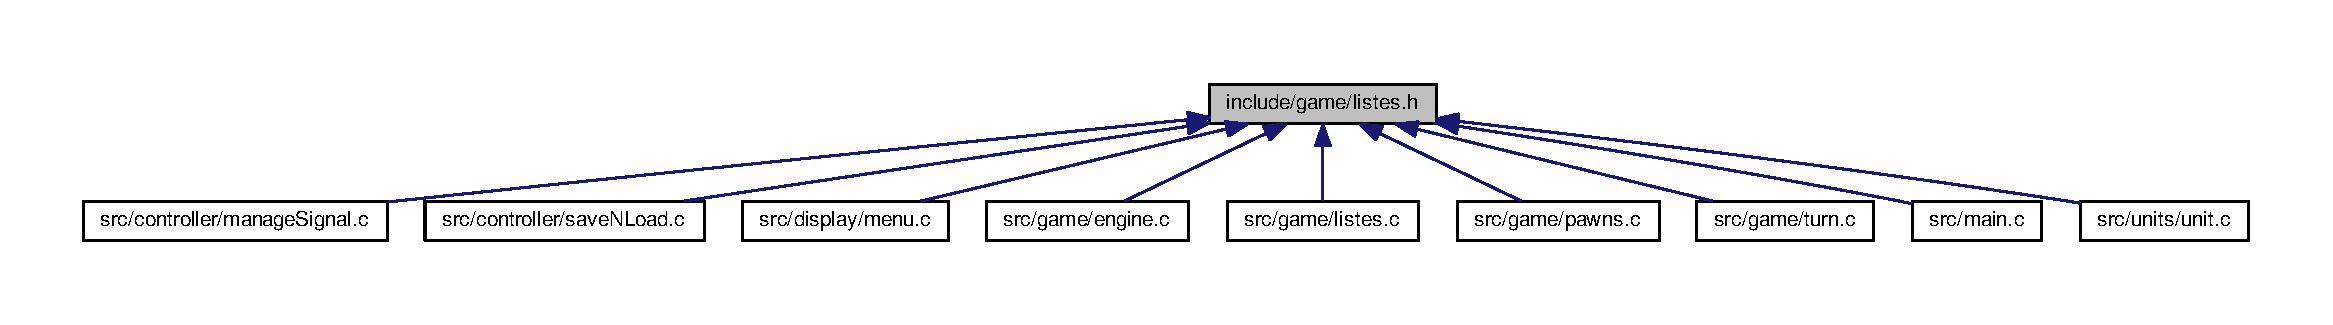
\includegraphics[width=350pt]{listes_8h__dep__incl}
\end{center}
\end{figure}
\subsection*{Macros}
\begin{DoxyCompactItemize}
\item 
\hypertarget{listes_8h_a787bfbe1eb9dcefcecee22f8470b42ac}{}\#define \hyperlink{listes_8h_a787bfbe1eb9dcefcecee22f8470b42ac}{M\+A\+X\+\_\+\+J\+O\+U\+E\+U\+R}~3\label{listes_8h_a787bfbe1eb9dcefcecee22f8470b42ac}

\begin{DoxyCompactList}\small\item\em Nombre max de listes. \end{DoxyCompactList}\end{DoxyCompactItemize}
\subsection*{Fonctions}
\begin{DoxyCompactItemize}
\item 
\hypertarget{listes_8h_a0650253bc6bb82ca23f4202fcc0b523f}{}void \hyperlink{listes_8h_a0650253bc6bb82ca23f4202fcc0b523f}{init\+\_\+liste} (int)\label{listes_8h_a0650253bc6bb82ca23f4202fcc0b523f}

\begin{DoxyCompactList}\small\item\em Initialise une liste. \end{DoxyCompactList}\item 
\hypertarget{listes_8h_aa5bc0ce3a17b5ee43e07b2d0c76c7263}{}void \hyperlink{listes_8h_aa5bc0ce3a17b5ee43e07b2d0c76c7263}{init\+Lists} ()\label{listes_8h_aa5bc0ce3a17b5ee43e07b2d0c76c7263}

\begin{DoxyCompactList}\small\item\em Initialise les listes. \end{DoxyCompactList}\item 
\hypertarget{listes_8h_a2b2eda6254a23ec34d4d3f1adc59e19c}{}int \hyperlink{listes_8h_a2b2eda6254a23ec34d4d3f1adc59e19c}{liste\+\_\+vide} (int)\label{listes_8h_a2b2eda6254a23ec34d4d3f1adc59e19c}

\begin{DoxyCompactList}\small\item\em Vérifie si une liste est vide. \end{DoxyCompactList}\item 
\hypertarget{listes_8h_a963773bb217fdd22fb30244a4e33b6b0}{}int \hyperlink{listes_8h_a963773bb217fdd22fb30244a4e33b6b0}{hors\+\_\+liste} (int)\label{listes_8h_a963773bb217fdd22fb30244a4e33b6b0}

\begin{DoxyCompactList}\small\item\em Vérifie si l\textquotesingle{}élément courant est hors de la liste. \end{DoxyCompactList}\item 
\hypertarget{listes_8h_a7fe8773e0a7479444f22bba1ac1f98b8}{}void \hyperlink{listes_8h_a7fe8773e0a7479444f22bba1ac1f98b8}{en\+\_\+tete} (int)\label{listes_8h_a7fe8773e0a7479444f22bba1ac1f98b8}

\begin{DoxyCompactList}\small\item\em Se met en tête de la liste. \end{DoxyCompactList}\item 
\hypertarget{listes_8h_afdcdb2634240b5fa64985f43ef1633f4}{}void \hyperlink{listes_8h_afdcdb2634240b5fa64985f43ef1633f4}{en\+\_\+queue} (int)\label{listes_8h_afdcdb2634240b5fa64985f43ef1633f4}

\begin{DoxyCompactList}\small\item\em Se met en queue de la liste. \end{DoxyCompactList}\item 
\hypertarget{listes_8h_ab26e83976c269c3ef19fc17a5469241b}{}void \hyperlink{listes_8h_ab26e83976c269c3ef19fc17a5469241b}{precedent} (int)\label{listes_8h_ab26e83976c269c3ef19fc17a5469241b}

\begin{DoxyCompactList}\small\item\em Se positionne sur l\textquotesingle{}élément précédent. \end{DoxyCompactList}\item 
\hypertarget{listes_8h_a55ef1c7d379cfa1c1fcbefae37afb1a6}{}void \hyperlink{listes_8h_a55ef1c7d379cfa1c1fcbefae37afb1a6}{suivant} (int)\label{listes_8h_a55ef1c7d379cfa1c1fcbefae37afb1a6}

\begin{DoxyCompactList}\small\item\em Se positionne sur l\textquotesingle{}élément suivant. \end{DoxyCompactList}\item 
\hypertarget{listes_8h_a7623030aadf16e02e2117efc5535d214}{}void \hyperlink{listes_8h_a7623030aadf16e02e2117efc5535d214}{valeur\+\_\+elt} (int, \hyperlink{structvector}{vector} $\ast$v)\label{listes_8h_a7623030aadf16e02e2117efc5535d214}

\begin{DoxyCompactList}\small\item\em Récupère la valeur de l\textquotesingle{}élément. \end{DoxyCompactList}\item 
\hypertarget{listes_8h_a90e250311850f4c70f83eae9088b8e70}{}void \hyperlink{listes_8h_a90e250311850f4c70f83eae9088b8e70}{modif\+\_\+elt} (int, \hyperlink{structvector}{vector} v)\label{listes_8h_a90e250311850f4c70f83eae9088b8e70}

\begin{DoxyCompactList}\small\item\em Modifie la valeur de l\textquotesingle{}élément. \end{DoxyCompactList}\item 
\hypertarget{listes_8h_a3049385b47a41d5f199cb7fb92c01ea2}{}void \hyperlink{listes_8h_a3049385b47a41d5f199cb7fb92c01ea2}{oter\+\_\+elt} (int)\label{listes_8h_a3049385b47a41d5f199cb7fb92c01ea2}

\begin{DoxyCompactList}\small\item\em Supprime l\textquotesingle{}élément. \end{DoxyCompactList}\item 
\hypertarget{listes_8h_afd195b1e782c46676b25dae2acd0dcfd}{}void \hyperlink{listes_8h_afd195b1e782c46676b25dae2acd0dcfd}{ajout\+\_\+droit} (int, \hyperlink{structvector}{vector} v)\label{listes_8h_afd195b1e782c46676b25dae2acd0dcfd}

\begin{DoxyCompactList}\small\item\em Ajoute à droite l\textquotesingle{}élément. \end{DoxyCompactList}\item 
\hypertarget{listes_8h_aa4212e845f5b58a494b7bf1ee3f966c6}{}void \hyperlink{listes_8h_aa4212e845f5b58a494b7bf1ee3f966c6}{ajout\+\_\+gauche} (int, \hyperlink{structvector}{vector} v)\label{listes_8h_aa4212e845f5b58a494b7bf1ee3f966c6}

\begin{DoxyCompactList}\small\item\em Ajoute à gauche l\textquotesingle{}élément. \end{DoxyCompactList}\item 
void \hyperlink{listes_8h_aa690a04ce7dc898d9b5b812905c8eedd}{dump\+List} (short nb\+List)
\begin{DoxyCompactList}\small\item\em Vide une liste. \end{DoxyCompactList}\item 
void \hyperlink{listes_8h_af168e9ee606d470e92ae65ac69628808}{dump\+All\+Lists} ()
\begin{DoxyCompactList}\small\item\em Vide les listes. \end{DoxyCompactList}\item 
void \hyperlink{listes_8h_a2c34e2f98b6cefbb83c1f2879f9a4e55}{add\+Unit} (\hyperlink{structvector}{vector} coord\+Unit)
\begin{DoxyCompactList}\small\item\em Ajoute une unité \end{DoxyCompactList}\item 
void \hyperlink{listes_8h_af2ebc85ca89d3d03e90a50c0e2b77339}{destroy\+Unit} (\hyperlink{structvector}{vector} coord\+Unit)
\begin{DoxyCompactList}\small\item\em Détruit une unité \end{DoxyCompactList}\item 
void \hyperlink{listes_8h_a0f4c61706f0b5b091b3a4ee201f5e69a}{print\+List} (short num\+List)
\begin{DoxyCompactList}\small\item\em Affiche la liste. \end{DoxyCompactList}\item 
int \hyperlink{listes_8h_a0171ca43abde0218c78caa6687eadf53}{count\+Units} ()
\begin{DoxyCompactList}\small\item\em Compte le nombre d\textquotesingle{}unités. \end{DoxyCompactList}\item 
void \hyperlink{listes_8h_ae0388407b6344914c4167f5ae477413e}{add\+Target} (\hyperlink{engine_8h_af7667555c2dcfbdd55ec3e9dd6a907ba}{unit\+Name} name, \hyperlink{structvector}{vector} coord\+Unit)
\begin{DoxyCompactList}\small\item\em Ajoute une cible. \end{DoxyCompactList}\item 
bool \hyperlink{listes_8h_a7a89e1a5008f1b3bb21980f812fd7c28}{search\+Target} (int num\+List, \hyperlink{structvector}{vector} coord\+Target)
\begin{DoxyCompactList}\small\item\em Cherche une cible. \end{DoxyCompactList}\end{DoxyCompactItemize}
\subsection*{Variables}
\begin{DoxyCompactItemize}
\item 
int \hyperlink{listes_8h_a4523d7d0657b5558fe454f142b9411d8}{target\+List}
\begin{DoxyCompactList}\small\item\em Cibles potentielles. \end{DoxyCompactList}\end{DoxyCompactItemize}


\subsection{Description détaillée}
En-\/tête listes de vecteurs. 

\begin{DoxyAuthor}{Auteur}
Cousin Brandon Chaudemanche Ewen Biardeau Tristan 
\end{DoxyAuthor}
\begin{DoxyVersion}{Version}
v1.\+00 
\end{DoxyVersion}
\begin{DoxyDate}{Date}
18/12/2015 
\end{DoxyDate}


\subsection{Documentation des fonctions}
\hypertarget{listes_8h_ae0388407b6344914c4167f5ae477413e}{}\index{listes.\+h@{listes.\+h}!add\+Target@{add\+Target}}
\index{add\+Target@{add\+Target}!listes.\+h@{listes.\+h}}
\subsubsection[{add\+Target}]{\setlength{\rightskip}{0pt plus 5cm}void add\+Target (
\begin{DoxyParamCaption}
\item[{{\bf unit\+Name}}]{name, }
\item[{{\bf vector}}]{coord\+Unit}
\end{DoxyParamCaption}
)}\label{listes_8h_ae0388407b6344914c4167f5ae477413e}


Ajoute une cible. 

Ajoute une cible.


\begin{DoxyParams}{Paramètres}
{\em name} & Nom de l\textquotesingle{}unité \\
\hline
{\em coord\+Unit} & Coordonnées de l\textquotesingle{}unité \\
\hline
\end{DoxyParams}


Définition à la ligne 211 du fichier listes.\+c.

\hypertarget{listes_8h_a2c34e2f98b6cefbb83c1f2879f9a4e55}{}\index{listes.\+h@{listes.\+h}!add\+Unit@{add\+Unit}}
\index{add\+Unit@{add\+Unit}!listes.\+h@{listes.\+h}}
\subsubsection[{add\+Unit}]{\setlength{\rightskip}{0pt plus 5cm}void add\+Unit (
\begin{DoxyParamCaption}
\item[{{\bf vector}}]{coord\+Unit}
\end{DoxyParamCaption}
)}\label{listes_8h_a2c34e2f98b6cefbb83c1f2879f9a4e55}


Ajoute une unité 

Ajoute une unité


\begin{DoxyParams}{Paramètres}
{\em coord\+Unit} & Coordonnées de l\textquotesingle{}unité \\
\hline
\end{DoxyParams}


Définition à la ligne 179 du fichier listes.\+c.

\hypertarget{listes_8h_a0171ca43abde0218c78caa6687eadf53}{}\index{listes.\+h@{listes.\+h}!count\+Units@{count\+Units}}
\index{count\+Units@{count\+Units}!listes.\+h@{listes.\+h}}
\subsubsection[{count\+Units}]{\setlength{\rightskip}{0pt plus 5cm}int count\+Units (
\begin{DoxyParamCaption}
{}
\end{DoxyParamCaption}
)}\label{listes_8h_a0171ca43abde0218c78caa6687eadf53}


Compte le nombre d\textquotesingle{}unités. 

Compte le nombre d\textquotesingle{}unités.

\begin{DoxyReturn}{Renvoie}
Retourne le nombre d\textquotesingle{}unité 
\end{DoxyReturn}


Définition à la ligne 280 du fichier listes.\+c.

\hypertarget{listes_8h_af2ebc85ca89d3d03e90a50c0e2b77339}{}\index{listes.\+h@{listes.\+h}!destroy\+Unit@{destroy\+Unit}}
\index{destroy\+Unit@{destroy\+Unit}!listes.\+h@{listes.\+h}}
\subsubsection[{destroy\+Unit}]{\setlength{\rightskip}{0pt plus 5cm}void destroy\+Unit (
\begin{DoxyParamCaption}
\item[{{\bf vector}}]{coord\+Unit}
\end{DoxyParamCaption}
)}\label{listes_8h_af2ebc85ca89d3d03e90a50c0e2b77339}


Détruit une unité 

Détruit une unité


\begin{DoxyParams}{Paramètres}
{\em coord\+Unit} & Coordonnées de l\textquotesingle{}unité à détruire \\
\hline
\end{DoxyParams}


Définition à la ligne 260 du fichier listes.\+c.

\hypertarget{listes_8h_af168e9ee606d470e92ae65ac69628808}{}\index{listes.\+h@{listes.\+h}!dump\+All\+Lists@{dump\+All\+Lists}}
\index{dump\+All\+Lists@{dump\+All\+Lists}!listes.\+h@{listes.\+h}}
\subsubsection[{dump\+All\+Lists}]{\setlength{\rightskip}{0pt plus 5cm}void dump\+All\+Lists (
\begin{DoxyParamCaption}
{}
\end{DoxyParamCaption}
)}\label{listes_8h_af168e9ee606d470e92ae65ac69628808}


Vide les listes. 

Vide les listes. 

Définition à la ligne 167 du fichier listes.\+c.

\hypertarget{listes_8h_aa690a04ce7dc898d9b5b812905c8eedd}{}\index{listes.\+h@{listes.\+h}!dump\+List@{dump\+List}}
\index{dump\+List@{dump\+List}!listes.\+h@{listes.\+h}}
\subsubsection[{dump\+List}]{\setlength{\rightskip}{0pt plus 5cm}void dump\+List (
\begin{DoxyParamCaption}
\item[{short}]{nb\+List}
\end{DoxyParamCaption}
)}\label{listes_8h_aa690a04ce7dc898d9b5b812905c8eedd}


Vide une liste. 


\begin{DoxyParams}{Paramètres}
{\em nb\+List} & Numéro de la liste à vider \\
\hline
\end{DoxyParams}


Définition à la ligne 155 du fichier listes.\+c.

\hypertarget{listes_8h_a0f4c61706f0b5b091b3a4ee201f5e69a}{}\index{listes.\+h@{listes.\+h}!print\+List@{print\+List}}
\index{print\+List@{print\+List}!listes.\+h@{listes.\+h}}
\subsubsection[{print\+List}]{\setlength{\rightskip}{0pt plus 5cm}void print\+List (
\begin{DoxyParamCaption}
\item[{short}]{num\+List}
\end{DoxyParamCaption}
)}\label{listes_8h_a0f4c61706f0b5b091b3a4ee201f5e69a}


Affiche la liste. 

Affiche la liste.


\begin{DoxyParams}{Paramètres}
{\em num\+List} & Numéro de liste \\
\hline
\end{DoxyParams}


Définition à la ligne 222 du fichier listes.\+c.

\hypertarget{listes_8h_a7a89e1a5008f1b3bb21980f812fd7c28}{}\index{listes.\+h@{listes.\+h}!search\+Target@{search\+Target}}
\index{search\+Target@{search\+Target}!listes.\+h@{listes.\+h}}
\subsubsection[{search\+Target}]{\setlength{\rightskip}{0pt plus 5cm}bool search\+Target (
\begin{DoxyParamCaption}
\item[{int}]{num\+List, }
\item[{{\bf vector}}]{coord\+Target}
\end{DoxyParamCaption}
)}\label{listes_8h_a7a89e1a5008f1b3bb21980f812fd7c28}


Cherche une cible. 

Cherche une cible.


\begin{DoxyParams}{Paramètres}
{\em num\+List} & Numéro de la liste \\
\hline
{\em coord\+Target} & Coordonnées de la cible \\
\hline
\end{DoxyParams}
\begin{DoxyReturn}{Renvoie}
Retourne vrai si cible trouvée 
\end{DoxyReturn}


Définition à la ligne 301 du fichier listes.\+c.



\subsection{Documentation des variables}
\hypertarget{listes_8h_a4523d7d0657b5558fe454f142b9411d8}{}\index{listes.\+h@{listes.\+h}!target\+List@{target\+List}}
\index{target\+List@{target\+List}!listes.\+h@{listes.\+h}}
\subsubsection[{target\+List}]{\setlength{\rightskip}{0pt plus 5cm}int target\+List}\label{listes_8h_a4523d7d0657b5558fe454f142b9411d8}


Cibles potentielles. 

Cibles potentielles. 

Définition à la ligne 28 du fichier listes.\+c.


\hypertarget{pathList_8h}{}\section{Référence du fichier include/game/path\+List.h}
\label{pathList_8h}\index{include/game/path\+List.\+h@{include/game/path\+List.\+h}}


En-\/tête listes des chemins.  


Ce graphe montre quels fichiers incluent directement ou indirectement ce fichier \+:\nopagebreak
\begin{figure}[H]
\begin{center}
\leavevmode
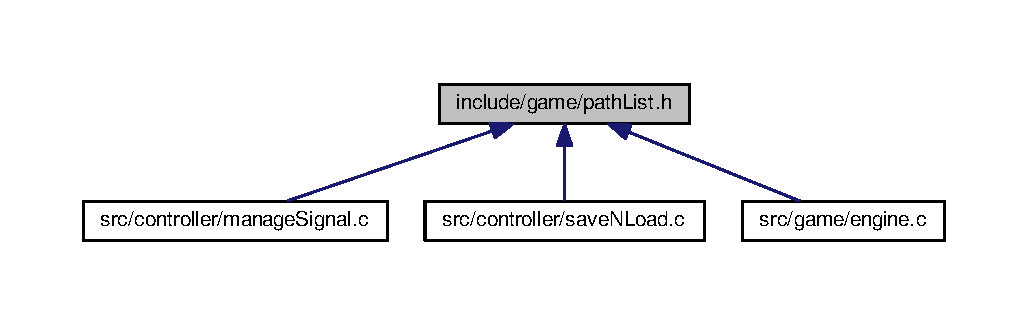
\includegraphics[width=350pt]{pathList_8h__dep__incl}
\end{center}
\end{figure}
\subsection*{Fonctions}
\begin{DoxyCompactItemize}
\item 
void \hyperlink{pathList_8h_a6a2e00dafeb02729bb43a51b048f2b11}{init\+Path} (int)
\begin{DoxyCompactList}\small\item\em Initialise le chemin. \end{DoxyCompactList}\item 
\hypertarget{pathList_8h_aca469a8527a0bc92e66306a1c8ada185}{}void \hyperlink{pathList_8h_aca469a8527a0bc92e66306a1c8ada185}{init\+Paths} ()\label{pathList_8h_aca469a8527a0bc92e66306a1c8ada185}

\begin{DoxyCompactList}\small\item\em Initialise les chemins. \end{DoxyCompactList}\item 
int \hyperlink{pathList_8h_a2aab13e3009ebe3949a32c10c03adcd8}{empty\+Path} (int n)
\begin{DoxyCompactList}\small\item\em Vérifie si chemin vide. \end{DoxyCompactList}\item 
int \hyperlink{pathList_8h_a4bcf1b8579c9a03c9070e33c77993426}{out\+Path} (int n)
\begin{DoxyCompactList}\small\item\em Vérifie si l\textquotesingle{}élément courant est en dehors de la liste. \end{DoxyCompactList}\item 
void \hyperlink{pathList_8h_af5f66b0e2d9ff7dd44fdd821bb9377cf}{path\+Head} (int n)
\begin{DoxyCompactList}\small\item\em Se met en tête de la liste. \end{DoxyCompactList}\item 
void \hyperlink{pathList_8h_a58814bcfb1182201bbecf88f839cd0f7}{path\+Tail} (int n)
\begin{DoxyCompactList}\small\item\em Se met en queue de la liste. \end{DoxyCompactList}\item 
void \hyperlink{pathList_8h_a2e1e62efbdb494f85de87088a068c916}{previous} (int n)
\begin{DoxyCompactList}\small\item\em Se positionne sur l\textquotesingle{}élément précédent. \end{DoxyCompactList}\item 
void \hyperlink{pathList_8h_ae29c8124809dc534b7ff12214d16183c}{next} (int n)
\begin{DoxyCompactList}\small\item\em Se positionne sur l\textquotesingle{}élément suivant. \end{DoxyCompactList}\item 
void \hyperlink{pathList_8h_affe2967c536ca680e1389c746dc2d944}{get\+Tile} (int n, \hyperlink{structvector}{vector} $\ast$v, int $\ast$F)
\begin{DoxyCompactList}\small\item\em Récupère la valeur d\textquotesingle{}une case. \end{DoxyCompactList}\item 
void \hyperlink{pathList_8h_afac156c3a2eedf22deaae38595f95a65}{set\+Tile} (int n, \hyperlink{structvector}{vector} v, int F)
\begin{DoxyCompactList}\small\item\em Modifie la valeur d\textquotesingle{}une case. \end{DoxyCompactList}\item 
void \hyperlink{pathList_8h_acb403a99e156dd37be05e5d1245ca591}{erase\+Tile} (int n)
\begin{DoxyCompactList}\small\item\em Efface une case. \end{DoxyCompactList}\item 
void \hyperlink{pathList_8h_add77d77457e5c3b5e5e3ba1574e1e706}{to\+Right\+Path} (int n, \hyperlink{structvector}{vector} v, int F)
\begin{DoxyCompactList}\small\item\em Ajoute une case à droite. \end{DoxyCompactList}\item 
void \hyperlink{pathList_8h_afd17fd81ff6e16ee988340ae898ba362}{dump\+Path} (short nb\+List)
\begin{DoxyCompactList}\small\item\em Vide le chemin. \end{DoxyCompactList}\item 
void \hyperlink{pathList_8h_a18154e93d817c730195d7fa04bd6c1d3}{dump\+All\+Paths} ()
\begin{DoxyCompactList}\small\item\em Vide les chemins. \end{DoxyCompactList}\item 
bool \hyperlink{pathList_8h_a3415787bd9e4aa84fb3f770c44de5275}{search\+Tile} (int n, \hyperlink{structvector}{vector})
\begin{DoxyCompactList}\small\item\em Cherche une case. \end{DoxyCompactList}\item 
\hyperlink{structvector}{vector} \hyperlink{pathList_8h_ae36257ead315faab602c58a4a2ae19fc}{get\+Current\+Node} (int n)
\begin{DoxyCompactList}\small\item\em Récupère la case ayant le plus petit poids. \end{DoxyCompactList}\item 
void \hyperlink{pathList_8h_a2d3c6547f1a7f48cada640491d9f8903}{add\+Close\+List} (\hyperlink{structvector}{vector}, int)
\begin{DoxyCompactList}\small\item\em Ajoute la case à la liste fermée. \end{DoxyCompactList}\item 
void \hyperlink{pathList_8h_acf21882e0305b7855f4558e5f7803a49}{add\+Open\+List} (\hyperlink{structvector}{vector}, int)
\begin{DoxyCompactList}\small\item\em Ajoute la case à la liste ouverte. \end{DoxyCompactList}\end{DoxyCompactItemize}


\subsection{Description détaillée}
En-\/tête listes des chemins. 

\begin{DoxyAuthor}{Auteur}
Cousin Brandon Chaudemanche Ewen Biardeau Tristan 
\end{DoxyAuthor}
\begin{DoxyVersion}{Version}
v1.\+00 
\end{DoxyVersion}
\begin{DoxyDate}{Date}
18/12/2015 
\end{DoxyDate}


\subsection{Documentation des fonctions}
\hypertarget{pathList_8h_a2d3c6547f1a7f48cada640491d9f8903}{}\index{path\+List.\+h@{path\+List.\+h}!add\+Close\+List@{add\+Close\+List}}
\index{add\+Close\+List@{add\+Close\+List}!path\+List.\+h@{path\+List.\+h}}
\subsubsection[{add\+Close\+List}]{\setlength{\rightskip}{0pt plus 5cm}void add\+Close\+List (
\begin{DoxyParamCaption}
\item[{{\bf vector}}]{current, }
\item[{int}]{F}
\end{DoxyParamCaption}
)}\label{pathList_8h_a2d3c6547f1a7f48cada640491d9f8903}


Ajoute la case à la liste fermée. 

Ajoute la case à la liste fermée.


\begin{DoxyParams}{Paramètres}
{\em current} & Destination \\
\hline
{\em F} & Poids de la case \\
\hline
\end{DoxyParams}


Définition à la ligne 262 du fichier path\+List.\+c.

\hypertarget{pathList_8h_acf21882e0305b7855f4558e5f7803a49}{}\index{path\+List.\+h@{path\+List.\+h}!add\+Open\+List@{add\+Open\+List}}
\index{add\+Open\+List@{add\+Open\+List}!path\+List.\+h@{path\+List.\+h}}
\subsubsection[{add\+Open\+List}]{\setlength{\rightskip}{0pt plus 5cm}void add\+Open\+List (
\begin{DoxyParamCaption}
\item[{{\bf vector}}]{current, }
\item[{int}]{F}
\end{DoxyParamCaption}
)}\label{pathList_8h_acf21882e0305b7855f4558e5f7803a49}


Ajoute la case à la liste ouverte. 

Ajoute la case à la liste ouverte.


\begin{DoxyParams}{Paramètres}
{\em current} & Destination \\
\hline
{\em F} & Poids de la case \\
\hline
\end{DoxyParams}


Définition à la ligne 285 du fichier path\+List.\+c.

\hypertarget{pathList_8h_a18154e93d817c730195d7fa04bd6c1d3}{}\index{path\+List.\+h@{path\+List.\+h}!dump\+All\+Paths@{dump\+All\+Paths}}
\index{dump\+All\+Paths@{dump\+All\+Paths}!path\+List.\+h@{path\+List.\+h}}
\subsubsection[{dump\+All\+Paths}]{\setlength{\rightskip}{0pt plus 5cm}void dump\+All\+Paths (
\begin{DoxyParamCaption}
{}
\end{DoxyParamCaption}
)}\label{pathList_8h_a18154e93d817c730195d7fa04bd6c1d3}


Vide les chemins. 

Vide les chemins. 

Définition à la ligne 226 du fichier path\+List.\+c.

\hypertarget{pathList_8h_afd17fd81ff6e16ee988340ae898ba362}{}\index{path\+List.\+h@{path\+List.\+h}!dump\+Path@{dump\+Path}}
\index{dump\+Path@{dump\+Path}!path\+List.\+h@{path\+List.\+h}}
\subsubsection[{dump\+Path}]{\setlength{\rightskip}{0pt plus 5cm}void dump\+Path (
\begin{DoxyParamCaption}
\item[{short}]{nb\+List}
\end{DoxyParamCaption}
)}\label{pathList_8h_afd17fd81ff6e16ee988340ae898ba362}


Vide le chemin. 

Vide le chemin.


\begin{DoxyParams}{Paramètres}
{\em nb\+List} & Numéro de la liste à vider \\
\hline
\end{DoxyParams}


Définition à la ligne 214 du fichier path\+List.\+c.

\hypertarget{pathList_8h_a2aab13e3009ebe3949a32c10c03adcd8}{}\index{path\+List.\+h@{path\+List.\+h}!empty\+Path@{empty\+Path}}
\index{empty\+Path@{empty\+Path}!path\+List.\+h@{path\+List.\+h}}
\subsubsection[{empty\+Path}]{\setlength{\rightskip}{0pt plus 5cm}int empty\+Path (
\begin{DoxyParamCaption}
\item[{int}]{n}
\end{DoxyParamCaption}
)}\label{pathList_8h_a2aab13e3009ebe3949a32c10c03adcd8}


Vérifie si chemin vide. 

Vérifie si chemin vide.


\begin{DoxyParams}{Paramètres}
{\em n} & Chemin \\
\hline
\end{DoxyParams}
\begin{DoxyReturn}{Renvoie}
Retourne le drapeau si pas vide 
\end{DoxyReturn}


Définition à la ligne 54 du fichier path\+List.\+c.

\hypertarget{pathList_8h_acb403a99e156dd37be05e5d1245ca591}{}\index{path\+List.\+h@{path\+List.\+h}!erase\+Tile@{erase\+Tile}}
\index{erase\+Tile@{erase\+Tile}!path\+List.\+h@{path\+List.\+h}}
\subsubsection[{erase\+Tile}]{\setlength{\rightskip}{0pt plus 5cm}void erase\+Tile (
\begin{DoxyParamCaption}
\item[{int}]{n}
\end{DoxyParamCaption}
)}\label{pathList_8h_acb403a99e156dd37be05e5d1245ca591}


Efface une case. 

Efface une case.


\begin{DoxyParams}{Paramètres}
{\em n} & Liste \\
\hline
\end{DoxyParams}


Définition à la ligne 170 du fichier path\+List.\+c.

\hypertarget{pathList_8h_ae36257ead315faab602c58a4a2ae19fc}{}\index{path\+List.\+h@{path\+List.\+h}!get\+Current\+Node@{get\+Current\+Node}}
\index{get\+Current\+Node@{get\+Current\+Node}!path\+List.\+h@{path\+List.\+h}}
\subsubsection[{get\+Current\+Node}]{\setlength{\rightskip}{0pt plus 5cm}{\bf vector} get\+Current\+Node (
\begin{DoxyParamCaption}
\item[{int}]{n}
\end{DoxyParamCaption}
)}\label{pathList_8h_ae36257ead315faab602c58a4a2ae19fc}


Récupère la case ayant le plus petit poids. 

Récupère la case ayant le plus petit poids.


\begin{DoxyParams}{Paramètres}
{\em n} & Liste dans laquelle chercher \\
\hline
\end{DoxyParams}


Définition à la ligne 130 du fichier path\+List.\+c.

\hypertarget{pathList_8h_affe2967c536ca680e1389c746dc2d944}{}\index{path\+List.\+h@{path\+List.\+h}!get\+Tile@{get\+Tile}}
\index{get\+Tile@{get\+Tile}!path\+List.\+h@{path\+List.\+h}}
\subsubsection[{get\+Tile}]{\setlength{\rightskip}{0pt plus 5cm}void get\+Tile (
\begin{DoxyParamCaption}
\item[{int}]{n, }
\item[{{\bf vector} $\ast$}]{v, }
\item[{int $\ast$}]{F}
\end{DoxyParamCaption}
)}\label{pathList_8h_affe2967c536ca680e1389c746dc2d944}


Récupère la valeur d\textquotesingle{}une case. 

Récupère la valeur d\textquotesingle{}une case.


\begin{DoxyParams}{Paramètres}
{\em n} & Chemin \\
\hline
{\em v} & Position de la case \\
\hline
{\em F} & Poids de la case \\
\hline
\end{DoxyParams}


Définition à la ligne 117 du fichier path\+List.\+c.

\hypertarget{pathList_8h_a6a2e00dafeb02729bb43a51b048f2b11}{}\index{path\+List.\+h@{path\+List.\+h}!init\+Path@{init\+Path}}
\index{init\+Path@{init\+Path}!path\+List.\+h@{path\+List.\+h}}
\subsubsection[{init\+Path}]{\setlength{\rightskip}{0pt plus 5cm}void init\+Path (
\begin{DoxyParamCaption}
\item[{int}]{n}
\end{DoxyParamCaption}
)}\label{pathList_8h_a6a2e00dafeb02729bb43a51b048f2b11}


Initialise le chemin. 


\begin{DoxyParams}{Paramètres}
{\em n} & Chemin \\
\hline
\end{DoxyParams}


Définition à la ligne 31 du fichier path\+List.\+c.

\hypertarget{pathList_8h_ae29c8124809dc534b7ff12214d16183c}{}\index{path\+List.\+h@{path\+List.\+h}!next@{next}}
\index{next@{next}!path\+List.\+h@{path\+List.\+h}}
\subsubsection[{next}]{\setlength{\rightskip}{0pt plus 5cm}void next (
\begin{DoxyParamCaption}
\item[{int}]{n}
\end{DoxyParamCaption}
)}\label{pathList_8h_ae29c8124809dc534b7ff12214d16183c}


Se positionne sur l\textquotesingle{}élément suivant. 

Se positionne sur l\textquotesingle{}élément suivant.


\begin{DoxyParams}{Paramètres}
{\em n} & Chemin \\
\hline
\end{DoxyParams}


Définition à la ligne 105 du fichier path\+List.\+c.

\hypertarget{pathList_8h_a4bcf1b8579c9a03c9070e33c77993426}{}\index{path\+List.\+h@{path\+List.\+h}!out\+Path@{out\+Path}}
\index{out\+Path@{out\+Path}!path\+List.\+h@{path\+List.\+h}}
\subsubsection[{out\+Path}]{\setlength{\rightskip}{0pt plus 5cm}int out\+Path (
\begin{DoxyParamCaption}
\item[{int}]{n}
\end{DoxyParamCaption}
)}\label{pathList_8h_a4bcf1b8579c9a03c9070e33c77993426}


Vérifie si l\textquotesingle{}élément courant est en dehors de la liste. 

Vérifie si l\textquotesingle{}élément courant est en dehors de la liste.


\begin{DoxyParams}{Paramètres}
{\em n} & Liste \\
\hline
\end{DoxyParams}
\begin{DoxyReturn}{Renvoie}
Retourne l\textquotesingle{}élément courant si pas hors liste 
\end{DoxyReturn}


Définition à la ligne 65 du fichier path\+List.\+c.

\hypertarget{pathList_8h_af5f66b0e2d9ff7dd44fdd821bb9377cf}{}\index{path\+List.\+h@{path\+List.\+h}!path\+Head@{path\+Head}}
\index{path\+Head@{path\+Head}!path\+List.\+h@{path\+List.\+h}}
\subsubsection[{path\+Head}]{\setlength{\rightskip}{0pt plus 5cm}void path\+Head (
\begin{DoxyParamCaption}
\item[{int}]{n}
\end{DoxyParamCaption}
)}\label{pathList_8h_af5f66b0e2d9ff7dd44fdd821bb9377cf}


Se met en tête de la liste. 

Se met en tête de la liste.


\begin{DoxyParams}{Paramètres}
{\em n} & Chemin \\
\hline
\end{DoxyParams}


Définition à la ligne 75 du fichier path\+List.\+c.

\hypertarget{pathList_8h_a58814bcfb1182201bbecf88f839cd0f7}{}\index{path\+List.\+h@{path\+List.\+h}!path\+Tail@{path\+Tail}}
\index{path\+Tail@{path\+Tail}!path\+List.\+h@{path\+List.\+h}}
\subsubsection[{path\+Tail}]{\setlength{\rightskip}{0pt plus 5cm}void path\+Tail (
\begin{DoxyParamCaption}
\item[{int}]{n}
\end{DoxyParamCaption}
)}\label{pathList_8h_a58814bcfb1182201bbecf88f839cd0f7}


Se met en queue de la liste. 

Se met en queue de la liste.


\begin{DoxyParams}{Paramètres}
{\em n} & Chemin \\
\hline
\end{DoxyParams}


Définition à la ligne 85 du fichier path\+List.\+c.

\hypertarget{pathList_8h_a2e1e62efbdb494f85de87088a068c916}{}\index{path\+List.\+h@{path\+List.\+h}!previous@{previous}}
\index{previous@{previous}!path\+List.\+h@{path\+List.\+h}}
\subsubsection[{previous}]{\setlength{\rightskip}{0pt plus 5cm}void previous (
\begin{DoxyParamCaption}
\item[{int}]{n}
\end{DoxyParamCaption}
)}\label{pathList_8h_a2e1e62efbdb494f85de87088a068c916}


Se positionne sur l\textquotesingle{}élément précédent. 


\begin{DoxyParams}{Paramètres}
{\em n} & Chemin \\
\hline
\end{DoxyParams}


Définition à la ligne 95 du fichier path\+List.\+c.

\hypertarget{pathList_8h_a3415787bd9e4aa84fb3f770c44de5275}{}\index{path\+List.\+h@{path\+List.\+h}!search\+Tile@{search\+Tile}}
\index{search\+Tile@{search\+Tile}!path\+List.\+h@{path\+List.\+h}}
\subsubsection[{search\+Tile}]{\setlength{\rightskip}{0pt plus 5cm}bool search\+Tile (
\begin{DoxyParamCaption}
\item[{int}]{n, }
\item[{{\bf vector}}]{coord\+Tile}
\end{DoxyParamCaption}
)}\label{pathList_8h_a3415787bd9e4aa84fb3f770c44de5275}


Cherche une case. 

Cherche une case.


\begin{DoxyParams}{Paramètres}
{\em n} & Liste \\
\hline
{\em coord\+Tile} & Position de la case \\
\hline
\end{DoxyParams}


Définition à la ligne 239 du fichier path\+List.\+c.

\hypertarget{pathList_8h_afac156c3a2eedf22deaae38595f95a65}{}\index{path\+List.\+h@{path\+List.\+h}!set\+Tile@{set\+Tile}}
\index{set\+Tile@{set\+Tile}!path\+List.\+h@{path\+List.\+h}}
\subsubsection[{set\+Tile}]{\setlength{\rightskip}{0pt plus 5cm}void set\+Tile (
\begin{DoxyParamCaption}
\item[{int}]{n, }
\item[{{\bf vector}}]{v, }
\item[{int}]{F}
\end{DoxyParamCaption}
)}\label{pathList_8h_afac156c3a2eedf22deaae38595f95a65}


Modifie la valeur d\textquotesingle{}une case. 

Modifie la valeur d\textquotesingle{}une case.


\begin{DoxyParams}{Paramètres}
{\em n} & Liste \\
\hline
{\em v} & Nouvelle position \\
\hline
{\em F} & Nouveau poids \\
\hline
\end{DoxyParams}


Définition à la ligne 157 du fichier path\+List.\+c.

\hypertarget{pathList_8h_add77d77457e5c3b5e5e3ba1574e1e706}{}\index{path\+List.\+h@{path\+List.\+h}!to\+Right\+Path@{to\+Right\+Path}}
\index{to\+Right\+Path@{to\+Right\+Path}!path\+List.\+h@{path\+List.\+h}}
\subsubsection[{to\+Right\+Path}]{\setlength{\rightskip}{0pt plus 5cm}void to\+Right\+Path (
\begin{DoxyParamCaption}
\item[{int}]{n, }
\item[{{\bf vector}}]{v, }
\item[{int}]{F}
\end{DoxyParamCaption}
)}\label{pathList_8h_add77d77457e5c3b5e5e3ba1574e1e706}


Ajoute une case à droite. 


\begin{DoxyParams}{Paramètres}
{\em n} & Liste \\
\hline
{\em v} & Position à ajouter \\
\hline
{\em F} & Poids à ajouter \\
\hline
\end{DoxyParams}


Définition à la ligne 191 du fichier path\+List.\+c.


\hypertarget{pawns_8h}{}\section{Référence du fichier include/game/pawns.h}
\label{pawns_8h}\index{include/game/pawns.\+h@{include/game/pawns.\+h}}


En-\/tête gestions des pions.  


Ce graphe montre quels fichiers incluent directement ou indirectement ce fichier \+:\nopagebreak
\begin{figure}[H]
\begin{center}
\leavevmode
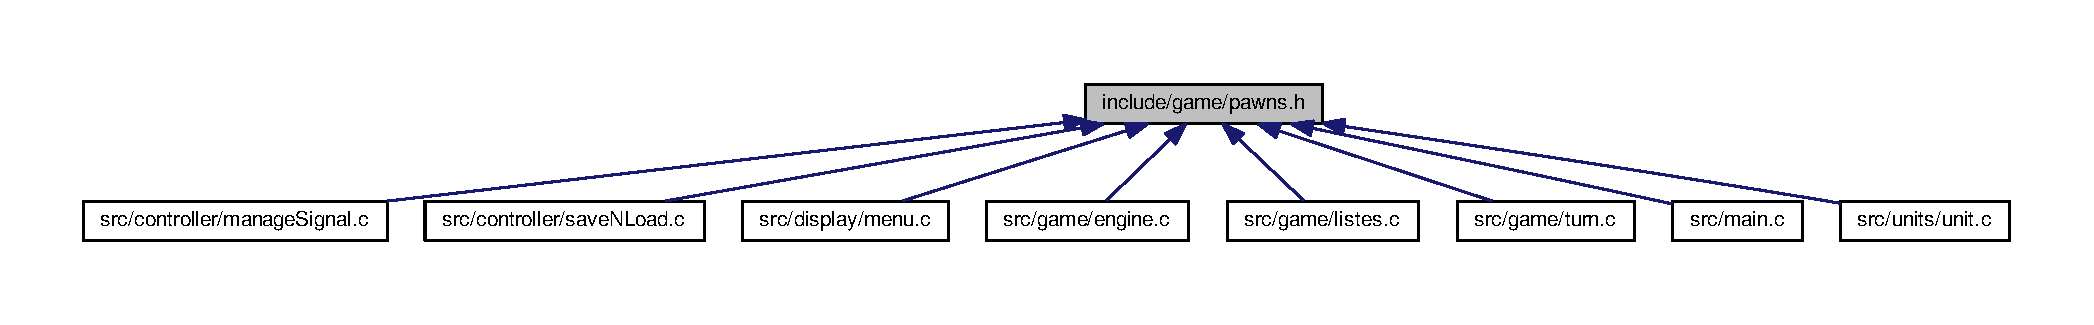
\includegraphics[width=350pt]{pawns_8h__dep__incl}
\end{center}
\end{figure}
\subsection*{Fonctions}
\begin{DoxyCompactItemize}
\item 
void \hyperlink{pawns_8h_af3226144d32d485e7e1362861b69ca11}{make\+Pawns} ()
\begin{DoxyCompactList}\small\item\em Crée les pions. \end{DoxyCompactList}\end{DoxyCompactItemize}
\subsection*{Variables}
\begin{DoxyCompactItemize}
\item 
\hyperlink{structunit}{unit} $\ast$ \hyperlink{pawns_8h_a0ec7c043ade24d330b48f393097f140f}{pawns}
\begin{DoxyCompactList}\small\item\em Tableaux des pions. \end{DoxyCompactList}\item 
\hypertarget{pawns_8h_a202e0786b273cb3b8e8cbe51ea8e3d1a}{}int \hyperlink{pawns_8h_a202e0786b273cb3b8e8cbe51ea8e3d1a}{size\+Pawns}\label{pawns_8h_a202e0786b273cb3b8e8cbe51ea8e3d1a}

\begin{DoxyCompactList}\small\item\em Nombre de pions. \end{DoxyCompactList}\end{DoxyCompactItemize}


\subsection{Description détaillée}
En-\/tête gestions des pions. 

\begin{DoxyAuthor}{Auteur}
Cousin Brandon Chaudemanche Ewen Biardeau Tristan 
\end{DoxyAuthor}
\begin{DoxyVersion}{Version}
v1.\+00 
\end{DoxyVersion}
\begin{DoxyDate}{Date}
18/12/2015 
\end{DoxyDate}


\subsection{Documentation des fonctions}
\hypertarget{pawns_8h_af3226144d32d485e7e1362861b69ca11}{}\index{pawns.\+h@{pawns.\+h}!make\+Pawns@{make\+Pawns}}
\index{make\+Pawns@{make\+Pawns}!pawns.\+h@{pawns.\+h}}
\subsubsection[{make\+Pawns}]{\setlength{\rightskip}{0pt plus 5cm}void make\+Pawns (
\begin{DoxyParamCaption}
{}
\end{DoxyParamCaption}
)}\label{pawns_8h_af3226144d32d485e7e1362861b69ca11}


Crée les pions. 

Crée les pions. 

Définition à la ligne 109 du fichier pawns.\+c.



\subsection{Documentation des variables}
\hypertarget{pawns_8h_a0ec7c043ade24d330b48f393097f140f}{}\index{pawns.\+h@{pawns.\+h}!pawns@{pawns}}
\index{pawns@{pawns}!pawns.\+h@{pawns.\+h}}
\subsubsection[{pawns}]{\setlength{\rightskip}{0pt plus 5cm}{\bf unit}$\ast$ pawns}\label{pawns_8h_a0ec7c043ade24d330b48f393097f140f}


Tableaux des pions. 

Tableaux des pions. 

Définition à la ligne 16 du fichier pawns.\+c.


\hypertarget{turn_8h}{}\section{Référence du fichier include/game/turn.h}
\label{turn_8h}\index{include/game/turn.\+h@{include/game/turn.\+h}}


En-\/tête gestion des tours.  


Ce graphe montre quels fichiers incluent directement ou indirectement ce fichier \+:\nopagebreak
\begin{figure}[H]
\begin{center}
\leavevmode
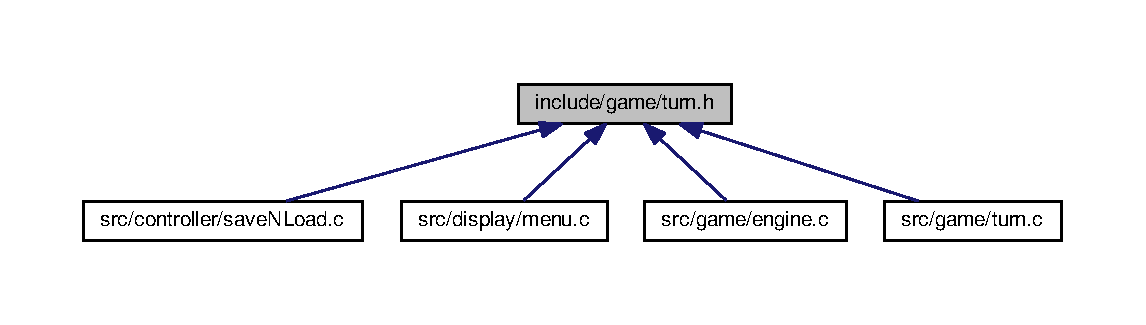
\includegraphics[width=350pt]{turn_8h__dep__incl}
\end{center}
\end{figure}
\subsection*{Macros}
\begin{DoxyCompactItemize}
\item 
\hypertarget{turn_8h_aaa58797f81bdb080460fcf48916ef5ac}{}\#define \hyperlink{turn_8h_aaa58797f81bdb080460fcf48916ef5ac}{T\+I\+M\+E\+\_\+\+B\+Y\+\_\+\+U\+N\+I\+T}~12\label{turn_8h_aaa58797f81bdb080460fcf48916ef5ac}

\begin{DoxyCompactList}\small\item\em Temps par unité possédée par le joueur. \end{DoxyCompactList}\item 
\hypertarget{turn_8h_a2cb9809f30ffec513e731194339f2ca4}{}\#define \hyperlink{turn_8h_a2cb9809f30ffec513e731194339f2ca4}{M\+I\+N\+\_\+\+T\+I\+M\+E}~60\label{turn_8h_a2cb9809f30ffec513e731194339f2ca4}

\begin{DoxyCompactList}\small\item\em Temps minimum par tour. \end{DoxyCompactList}\item 
\hypertarget{turn_8h_a5320d4457a472d8888ec1905bc0e0a1c}{}\#define \hyperlink{turn_8h_a5320d4457a472d8888ec1905bc0e0a1c}{M\+A\+X\+\_\+\+T\+I\+M\+E}~120\label{turn_8h_a5320d4457a472d8888ec1905bc0e0a1c}

\begin{DoxyCompactList}\small\item\em Temps maximum par tour. \end{DoxyCompactList}\end{DoxyCompactItemize}
\subsection*{Fonctions}
\begin{DoxyCompactItemize}
\item 
void \hyperlink{turn_8h_af77ebb54a900a2ef4a15ea354ff60f85}{play\+Turn} ()
\begin{DoxyCompactList}\small\item\em Joue un tour. \end{DoxyCompactList}\item 
void \hyperlink{turn_8h_a0d63b19dd2910e04bc114a4572276601}{play\+Attack} ()
\begin{DoxyCompactList}\small\item\em Joue une attaque. \end{DoxyCompactList}\item 
void \hyperlink{turn_8h_af6050b30e522cb4218786756c972d804}{play\+Move} ()
\begin{DoxyCompactList}\small\item\em Joue une mouvement. \end{DoxyCompactList}\item 
void \hyperlink{turn_8h_ab4e21eee8105ce3f15cb490ce17225e8}{pass\+Turn} ()
\begin{DoxyCompactList}\small\item\em Passe le tour. \end{DoxyCompactList}\item 
void \hyperlink{turn_8h_a9d6b655a52683afe2f4cb87e3f64bc2e}{change\+Direction} ()
\begin{DoxyCompactList}\small\item\em Change la direction. \end{DoxyCompactList}\item 
bool \hyperlink{turn_8h_a2c1ed39b34b58552a4cba52a3f832d14}{has\+Play} ()
\begin{DoxyCompactList}\small\item\em Vérifie si une action a été effectuée. \end{DoxyCompactList}\item 
\hypertarget{turn_8h_a5032490db7416ec2004861d51acda9e2}{}void \hyperlink{turn_8h_a5032490db7416ec2004861d51acda9e2}{surrender} ()\label{turn_8h_a5032490db7416ec2004861d51acda9e2}

\begin{DoxyCompactList}\small\item\em Abandonne la partie. \end{DoxyCompactList}\end{DoxyCompactItemize}
\subsection*{Variables}
\begin{DoxyCompactItemize}
\item 
\hypertarget{turn_8h_a5849a680495b395c75c2269657d5d4a5}{}int \hyperlink{turn_8h_a5849a680495b395c75c2269657d5d4a5}{has\+Moved}\label{turn_8h_a5849a680495b395c75c2269657d5d4a5}

\begin{DoxyCompactList}\small\item\em Joueur a joué \end{DoxyCompactList}\item 
\hypertarget{turn_8h_a1fa6b4cfe1a42f3d14c8701782a8ae6f}{}int \hyperlink{turn_8h_a1fa6b4cfe1a42f3d14c8701782a8ae6f}{has\+Attacked}\label{turn_8h_a1fa6b4cfe1a42f3d14c8701782a8ae6f}

\begin{DoxyCompactList}\small\item\em Joueur a attaqué \end{DoxyCompactList}\item 
\hypertarget{turn_8h_a776a08ce69ed60e7178f5fab585b5936}{}int \hyperlink{turn_8h_a776a08ce69ed60e7178f5fab585b5936}{has\+Passed}\label{turn_8h_a776a08ce69ed60e7178f5fab585b5936}

\begin{DoxyCompactList}\small\item\em Joueur a passé son tour. \end{DoxyCompactList}\item 
\hypertarget{turn_8h_ab28ae3d21446f3eb01eeeab3002ad942}{}int \hyperlink{turn_8h_ab28ae3d21446f3eb01eeeab3002ad942}{has\+Surrender}\label{turn_8h_ab28ae3d21446f3eb01eeeab3002ad942}

\begin{DoxyCompactList}\small\item\em Joueur a abandonné la partie. \end{DoxyCompactList}\end{DoxyCompactItemize}


\subsection{Description détaillée}
En-\/tête gestion des tours. 

\begin{DoxyAuthor}{Auteur}
Cousin Brandon Chaudemanche Ewen Biardeau Tristan 
\end{DoxyAuthor}
\begin{DoxyVersion}{Version}
v1.\+00 
\end{DoxyVersion}
\begin{DoxyDate}{Date}
18/12/2015 
\end{DoxyDate}


\subsection{Documentation des fonctions}
\hypertarget{turn_8h_a9d6b655a52683afe2f4cb87e3f64bc2e}{}\index{turn.\+h@{turn.\+h}!change\+Direction@{change\+Direction}}
\index{change\+Direction@{change\+Direction}!turn.\+h@{turn.\+h}}
\subsubsection[{change\+Direction}]{\setlength{\rightskip}{0pt plus 5cm}void change\+Direction (
\begin{DoxyParamCaption}
{}
\end{DoxyParamCaption}
)}\label{turn_8h_a9d6b655a52683afe2f4cb87e3f64bc2e}


Change la direction. 

Change la direction. 

Définition à la ligne 57 du fichier turn.\+c.

\hypertarget{turn_8h_a2c1ed39b34b58552a4cba52a3f832d14}{}\index{turn.\+h@{turn.\+h}!has\+Play@{has\+Play}}
\index{has\+Play@{has\+Play}!turn.\+h@{turn.\+h}}
\subsubsection[{has\+Play}]{\setlength{\rightskip}{0pt plus 5cm}bool has\+Play (
\begin{DoxyParamCaption}
{}
\end{DoxyParamCaption}
)}\label{turn_8h_a2c1ed39b34b58552a4cba52a3f832d14}


Vérifie si une action a été effectuée. 

Vérifie si une action a été effectuée.

\begin{DoxyReturn}{Renvoie}
Retourne vrai si le joueur a joué sinon faux 
\end{DoxyReturn}


Définition à la ligne 245 du fichier turn.\+c.

\hypertarget{turn_8h_ab4e21eee8105ce3f15cb490ce17225e8}{}\index{turn.\+h@{turn.\+h}!pass\+Turn@{pass\+Turn}}
\index{pass\+Turn@{pass\+Turn}!turn.\+h@{turn.\+h}}
\subsubsection[{pass\+Turn}]{\setlength{\rightskip}{0pt plus 5cm}void pass\+Turn (
\begin{DoxyParamCaption}
{}
\end{DoxyParamCaption}
)}\label{turn_8h_ab4e21eee8105ce3f15cb490ce17225e8}


Passe le tour. 

Passe le tour. 

Définition à la ligne 235 du fichier turn.\+c.

\hypertarget{turn_8h_a0d63b19dd2910e04bc114a4572276601}{}\index{turn.\+h@{turn.\+h}!play\+Attack@{play\+Attack}}
\index{play\+Attack@{play\+Attack}!turn.\+h@{turn.\+h}}
\subsubsection[{play\+Attack}]{\setlength{\rightskip}{0pt plus 5cm}void play\+Attack (
\begin{DoxyParamCaption}
{}
\end{DoxyParamCaption}
)}\label{turn_8h_a0d63b19dd2910e04bc114a4572276601}


Joue une attaque. 

Joue une attaque. 

Définition à la ligne 104 du fichier turn.\+c.

\hypertarget{turn_8h_af6050b30e522cb4218786756c972d804}{}\index{turn.\+h@{turn.\+h}!play\+Move@{play\+Move}}
\index{play\+Move@{play\+Move}!turn.\+h@{turn.\+h}}
\subsubsection[{play\+Move}]{\setlength{\rightskip}{0pt plus 5cm}void play\+Move (
\begin{DoxyParamCaption}
{}
\end{DoxyParamCaption}
)}\label{turn_8h_af6050b30e522cb4218786756c972d804}


Joue une mouvement. 

Joue une mouvement. 

Définition à la ligne 177 du fichier turn.\+c.

\hypertarget{turn_8h_af77ebb54a900a2ef4a15ea354ff60f85}{}\index{turn.\+h@{turn.\+h}!play\+Turn@{play\+Turn}}
\index{play\+Turn@{play\+Turn}!turn.\+h@{turn.\+h}}
\subsubsection[{play\+Turn}]{\setlength{\rightskip}{0pt plus 5cm}void play\+Turn (
\begin{DoxyParamCaption}
{}
\end{DoxyParamCaption}
)}\label{turn_8h_af77ebb54a900a2ef4a15ea354ff60f85}


Joue un tour. 

Joue un tour. 

Définition à la ligne 272 du fichier turn.\+c.


\hypertarget{unit_8h}{}\section{Référence du fichier include/units/unit.h}
\label{unit_8h}\index{include/units/unit.\+h@{include/units/unit.\+h}}


En-\/tête gestion des unités.  


Ce graphe montre quels fichiers incluent directement ou indirectement ce fichier \+:\nopagebreak
\begin{figure}[H]
\begin{center}
\leavevmode
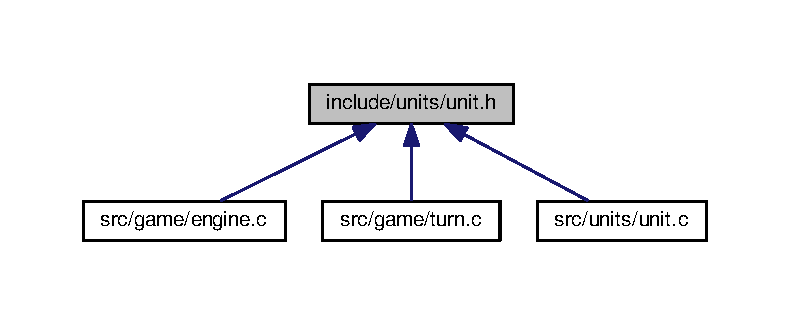
\includegraphics[width=350pt]{unit_8h__dep__incl}
\end{center}
\end{figure}
\subsection*{Fonctions}
\begin{DoxyCompactItemize}
\item 
bool \hyperlink{unit_8h_a85f8dfae2c8d83d9bc1b164adac6513d}{can\+Get\+Passed} (\hyperlink{structunit}{unit} $\ast$target)
\begin{DoxyCompactList}\small\item\em Vérifie si le passage est autorisé \end{DoxyCompactList}\item 
bool \hyperlink{unit_8h_ac194fc19a706dbd87e9a93c02b244f11}{can\+Block} (\hyperlink{structunit}{unit} $\ast$target)
\begin{DoxyCompactList}\small\item\em Vérifie si l\textquotesingle{}unité peut bloquer. \end{DoxyCompactList}\item 
bool \hyperlink{unit_8h_aa012dba081af99c4a666767c26ac1ac5}{can\+Attack} (\hyperlink{structunit}{unit} $\ast$target)
\begin{DoxyCompactList}\small\item\em Vérifie si l\textquotesingle{}unité peut attaquer. \end{DoxyCompactList}\item 
bool \hyperlink{unit_8h_a9c0738de90650e2f4640cae3bad4b3a2}{can\+Move} (\hyperlink{structunit}{unit} $\ast$target)
\begin{DoxyCompactList}\small\item\em Vérifie si l\textquotesingle{}unité peut bouger. \end{DoxyCompactList}\item 
bool \hyperlink{unit_8h_a52de919c7103012ce231d80e3bbe3e8d}{can\+Teleport} (\hyperlink{engine_8h_af7667555c2dcfbdd55ec3e9dd6a907ba}{unit\+Name} name)
\begin{DoxyCompactList}\small\item\em Vérifie si l\textquotesingle{}unité peut se téléporter. \end{DoxyCompactList}\item 
int \hyperlink{unit_8h_a5c8761ef40c541d75de80d6f6eeeb482}{get\+Side\+Attacked} (\hyperlink{structvector}{vector} source, \hyperlink{structvector}{vector} target)
\begin{DoxyCompactList}\small\item\em Récupère le côté attaqué \end{DoxyCompactList}\item 
void \hyperlink{unit_8h_a59537e7d55fc495b394087bf8a952d16}{heal} (\hyperlink{engine_8h_af7667555c2dcfbdd55ec3e9dd6a907ba}{unit\+Name} name)
\begin{DoxyCompactList}\small\item\em Soigne les unités. \end{DoxyCompactList}\item 
void \hyperlink{unit_8h_a6b948a17bbc3106f230c32a53121e6db}{attack} (\hyperlink{structvector}{vector} source, \hyperlink{structvector}{vector} target)
\begin{DoxyCompactList}\small\item\em Attaque une unité \end{DoxyCompactList}\item 
bool \hyperlink{unit_8h_a4004486abf500173fd3f51d2d3283275}{copy} (\hyperlink{structunit}{unit} $\ast$destination, \hyperlink{structunit}{unit} $\ast$source)
\begin{DoxyCompactList}\small\item\em Copie la structure source vers destination. \end{DoxyCompactList}\item 
void \hyperlink{unit_8h_a87c06ff9e86d3317e10387a5d5626f1a}{move} (\hyperlink{structvector}{vector} destination, \hyperlink{structvector}{vector} source)
\begin{DoxyCompactList}\small\item\em Bouge une unité \end{DoxyCompactList}\item 
void \hyperlink{unit_8h_ae52638eb8e2a94d1dd3df42c816681a3}{add\+Effect} (\hyperlink{structvector}{vector} target, \hyperlink{engine_8h_ac5ece9b6993cd3565502866b56317e84}{unit\+Effect} effect)
\begin{DoxyCompactList}\small\item\em Ajoute un effet à une unité \end{DoxyCompactList}\item 
void \hyperlink{unit_8h_a0e8d3997960e64de032d8c6592bb4dd4}{unit\+Init} (short \hyperlink{engine_8h_afaa2c64a9fd09c382394b57006c470ce}{no\+Player}, \hyperlink{structvector}{vector} coord\+Unit)
\begin{DoxyCompactList}\small\item\em Initialise une unité \end{DoxyCompactList}\item 
void \hyperlink{unit_8h_a10bfc9c0ad0c3d41388abf6e6b1c5135}{set\+Direction} (\hyperlink{structvector}{vector} coord\+Unit, int dir)
\begin{DoxyCompactList}\small\item\em Définis la direction d\textquotesingle{}une unité \end{DoxyCompactList}\item 
void \hyperlink{unit_8h_a956caa43f2ae1c1eecd5adb22062aed1}{erase} (\hyperlink{structunit}{unit} $\ast$)
\begin{DoxyCompactList}\small\item\em Efface une unité de la grille. \end{DoxyCompactList}\item 
bool \hyperlink{unit_8h_a8a36c4219ebbdb7f8566d00b5c7dbb2a}{is\+Sleeping} (\hyperlink{structvector}{vector})
\begin{DoxyCompactList}\small\item\em Vérifie si une unité est endormie. \end{DoxyCompactList}\item 
void \hyperlink{unit_8h_a505f360905b4ad0fa6e18f19405539ea}{recover} ()
\begin{DoxyCompactList}\small\item\em Se réveille tour par tour. \end{DoxyCompactList}\item 
bool \hyperlink{unit_8h_a04cb7c9ee636e575bfd9531780b829d7}{all\+Static} (int num\+Player)
\begin{DoxyCompactList}\small\item\em Vérifie si toutes les unités sont immobilisées. \end{DoxyCompactList}\item 
void \hyperlink{unit_8h_a1cbe53dd582c7ac03bafb0051a38a98b}{minus\+Effect} ()
\begin{DoxyCompactList}\small\item\em Diminue le temps de l\textquotesingle{}effet. \end{DoxyCompactList}\item 
void \hyperlink{unit_8h_afec10f9e98c70ab1915023cd0c8f76ca}{poison} ()
\begin{DoxyCompactList}\small\item\em Empoisonne une unité \end{DoxyCompactList}\item 
void \hyperlink{unit_8h_a4ea1b739c4b88857675c47d9960a69a4}{power\+Bonus} ()
\begin{DoxyCompactList}\small\item\em Octroie un bonus de puissance selon certaines conditions. \end{DoxyCompactList}\item 
void \hyperlink{unit_8h_a4ff80bc9cbc0a6e1e6e7a3936b8b48cb}{sleep} (\hyperlink{structvector}{vector})
\begin{DoxyCompactList}\small\item\em Endors une unité \end{DoxyCompactList}\end{DoxyCompactItemize}


\subsection{Description détaillée}
En-\/tête gestion des unités. 

\begin{DoxyAuthor}{Auteur}
Cousin Brandon Chaudemanche Ewen Biardeau Tristan 
\end{DoxyAuthor}
\begin{DoxyVersion}{Version}
v1.\+00 
\end{DoxyVersion}
\begin{DoxyDate}{Date}
18/12/2015 
\end{DoxyDate}


\subsection{Documentation des fonctions}
\hypertarget{unit_8h_ae52638eb8e2a94d1dd3df42c816681a3}{}\index{unit.\+h@{unit.\+h}!add\+Effect@{add\+Effect}}
\index{add\+Effect@{add\+Effect}!unit.\+h@{unit.\+h}}
\subsubsection[{add\+Effect}]{\setlength{\rightskip}{0pt plus 5cm}void add\+Effect (
\begin{DoxyParamCaption}
\item[{{\bf vector}}]{target, }
\item[{{\bf unit\+Effect}}]{effect}
\end{DoxyParamCaption}
)}\label{unit_8h_ae52638eb8e2a94d1dd3df42c816681a3}


Ajoute un effet à une unité 

Ajoute un effet à une unité


\begin{DoxyParams}{Paramètres}
{\em target} & Position unité cible \\
\hline
{\em effect} & Effet à appliquer sur la cible \\
\hline
\end{DoxyParams}


Définition à la ligne 437 du fichier unit.\+c.

\hypertarget{unit_8h_a04cb7c9ee636e575bfd9531780b829d7}{}\index{unit.\+h@{unit.\+h}!all\+Static@{all\+Static}}
\index{all\+Static@{all\+Static}!unit.\+h@{unit.\+h}}
\subsubsection[{all\+Static}]{\setlength{\rightskip}{0pt plus 5cm}bool all\+Static (
\begin{DoxyParamCaption}
\item[{int}]{num\+Player}
\end{DoxyParamCaption}
)}\label{unit_8h_a04cb7c9ee636e575bfd9531780b829d7}


Vérifie si toutes les unités sont immobilisées. 

Vérifie si toutes les unités sont immobilisées.


\begin{DoxyParams}{Paramètres}
{\em num\+Player} & Numéro du joueur \\
\hline
\end{DoxyParams}
\begin{DoxyReturn}{Renvoie}
Retourne vrai si toutes les unités sont immobilisés 
\end{DoxyReturn}


Définition à la ligne 529 du fichier unit.\+c.

\hypertarget{unit_8h_a6b948a17bbc3106f230c32a53121e6db}{}\index{unit.\+h@{unit.\+h}!attack@{attack}}
\index{attack@{attack}!unit.\+h@{unit.\+h}}
\subsubsection[{attack}]{\setlength{\rightskip}{0pt plus 5cm}void attack (
\begin{DoxyParamCaption}
\item[{{\bf vector}}]{source, }
\item[{{\bf vector}}]{target}
\end{DoxyParamCaption}
)}\label{unit_8h_a6b948a17bbc3106f230c32a53121e6db}


Attaque une unité 

Attaque une unité


\begin{DoxyParams}{Paramètres}
{\em source} & Unité attaquante \\
\hline
{\em target} & Unité cible \\
\hline
\end{DoxyParams}


Définition à la ligne 184 du fichier unit.\+c.

\hypertarget{unit_8h_aa012dba081af99c4a666767c26ac1ac5}{}\index{unit.\+h@{unit.\+h}!can\+Attack@{can\+Attack}}
\index{can\+Attack@{can\+Attack}!unit.\+h@{unit.\+h}}
\subsubsection[{can\+Attack}]{\setlength{\rightskip}{0pt plus 5cm}bool can\+Attack (
\begin{DoxyParamCaption}
\item[{{\bf unit} $\ast$}]{target}
\end{DoxyParamCaption}
)}\label{unit_8h_aa012dba081af99c4a666767c26ac1ac5}


Vérifie si l\textquotesingle{}unité peut attaquer. 

Vérifie si l\textquotesingle{}unité peut attaquer.


\begin{DoxyParams}{Paramètres}
{\em target} & Unité à analyser \\
\hline
\end{DoxyParams}
\begin{DoxyReturn}{Renvoie}
Retourne vrai si l\textquotesingle{}unité peut attaquer 
\end{DoxyReturn}


Définition à la ligne 86 du fichier unit.\+c.

\hypertarget{unit_8h_ac194fc19a706dbd87e9a93c02b244f11}{}\index{unit.\+h@{unit.\+h}!can\+Block@{can\+Block}}
\index{can\+Block@{can\+Block}!unit.\+h@{unit.\+h}}
\subsubsection[{can\+Block}]{\setlength{\rightskip}{0pt plus 5cm}bool can\+Block (
\begin{DoxyParamCaption}
\item[{{\bf unit} $\ast$}]{target}
\end{DoxyParamCaption}
)}\label{unit_8h_ac194fc19a706dbd87e9a93c02b244f11}


Vérifie si l\textquotesingle{}unité peut bloquer. 

Vérifie si l\textquotesingle{}unité peut bloquer.


\begin{DoxyParams}{Paramètres}
{\em target} & Unité à analyser \\
\hline
\end{DoxyParams}
\begin{DoxyReturn}{Renvoie}
Retourne vrai si l\textquotesingle{}unité peut bloquer 
\end{DoxyReturn}


Définition à la ligne 66 du fichier unit.\+c.

\hypertarget{unit_8h_a85f8dfae2c8d83d9bc1b164adac6513d}{}\index{unit.\+h@{unit.\+h}!can\+Get\+Passed@{can\+Get\+Passed}}
\index{can\+Get\+Passed@{can\+Get\+Passed}!unit.\+h@{unit.\+h}}
\subsubsection[{can\+Get\+Passed}]{\setlength{\rightskip}{0pt plus 5cm}bool can\+Get\+Passed (
\begin{DoxyParamCaption}
\item[{{\bf unit} $\ast$}]{target}
\end{DoxyParamCaption}
)}\label{unit_8h_a85f8dfae2c8d83d9bc1b164adac6513d}


Vérifie si le passage est autorisé 

Vérifie si le passage est autorisé


\begin{DoxyParams}{Paramètres}
{\em target} & Unité à analyser \\
\hline
\end{DoxyParams}
\begin{DoxyReturn}{Renvoie}
Retourne vrai si passage autorisé 
\end{DoxyReturn}


Définition à la ligne 46 du fichier unit.\+c.

\hypertarget{unit_8h_a9c0738de90650e2f4640cae3bad4b3a2}{}\index{unit.\+h@{unit.\+h}!can\+Move@{can\+Move}}
\index{can\+Move@{can\+Move}!unit.\+h@{unit.\+h}}
\subsubsection[{can\+Move}]{\setlength{\rightskip}{0pt plus 5cm}bool can\+Move (
\begin{DoxyParamCaption}
\item[{{\bf unit} $\ast$}]{target}
\end{DoxyParamCaption}
)}\label{unit_8h_a9c0738de90650e2f4640cae3bad4b3a2}


Vérifie si l\textquotesingle{}unité peut bouger. 

Vérifie si l\textquotesingle{}unité peut bouger.


\begin{DoxyParams}{Paramètres}
{\em target} & Unité à analyser \\
\hline
\end{DoxyParams}
\begin{DoxyReturn}{Renvoie}
Retourne vraie si l\textquotesingle{}unité peut se mouvoir 
\end{DoxyReturn}


Définition à la ligne 106 du fichier unit.\+c.

\hypertarget{unit_8h_a52de919c7103012ce231d80e3bbe3e8d}{}\index{unit.\+h@{unit.\+h}!can\+Teleport@{can\+Teleport}}
\index{can\+Teleport@{can\+Teleport}!unit.\+h@{unit.\+h}}
\subsubsection[{can\+Teleport}]{\setlength{\rightskip}{0pt plus 5cm}bool can\+Teleport (
\begin{DoxyParamCaption}
\item[{{\bf unit\+Name}}]{name}
\end{DoxyParamCaption}
)}\label{unit_8h_a52de919c7103012ce231d80e3bbe3e8d}


Vérifie si l\textquotesingle{}unité peut se téléporter. 

Vérifie si l\textquotesingle{}unité peut se téléporter.


\begin{DoxyParams}{Paramètres}
{\em name} & Nom de l\textquotesingle{}unité \\
\hline
\end{DoxyParams}
\begin{DoxyReturn}{Renvoie}
Retourne vraie si l\textquotesingle{}unité peut se déplacer 
\end{DoxyReturn}


Définition à la ligne 125 du fichier unit.\+c.

\hypertarget{unit_8h_a4004486abf500173fd3f51d2d3283275}{}\index{unit.\+h@{unit.\+h}!copy@{copy}}
\index{copy@{copy}!unit.\+h@{unit.\+h}}
\subsubsection[{copy}]{\setlength{\rightskip}{0pt plus 5cm}bool copy (
\begin{DoxyParamCaption}
\item[{{\bf unit} $\ast$}]{destination, }
\item[{{\bf unit} $\ast$}]{source}
\end{DoxyParamCaption}
)}\label{unit_8h_a4004486abf500173fd3f51d2d3283275}


Copie la structure source vers destination. 

Copie la structure source vers destination.


\begin{DoxyParams}{Paramètres}
{\em destination} & Structure destination \\
\hline
{\em source} & Structure source \\
\hline
\end{DoxyParams}
\begin{DoxyReturn}{Renvoie}
Retourne vrai si copie bien déroulée 
\end{DoxyReturn}


Définition à la ligne 236 du fichier unit.\+c.

\hypertarget{unit_8h_a956caa43f2ae1c1eecd5adb22062aed1}{}\index{unit.\+h@{unit.\+h}!erase@{erase}}
\index{erase@{erase}!unit.\+h@{unit.\+h}}
\subsubsection[{erase}]{\setlength{\rightskip}{0pt plus 5cm}void erase (
\begin{DoxyParamCaption}
\item[{{\bf unit} $\ast$}]{source}
\end{DoxyParamCaption}
)}\label{unit_8h_a956caa43f2ae1c1eecd5adb22062aed1}


Efface une unité de la grille. 


\begin{DoxyParams}{Paramètres}
{\em source} & Source à effacer \\
\hline
\end{DoxyParams}


Définition à la ligne 271 du fichier unit.\+c.

\hypertarget{unit_8h_a5c8761ef40c541d75de80d6f6eeeb482}{}\index{unit.\+h@{unit.\+h}!get\+Side\+Attacked@{get\+Side\+Attacked}}
\index{get\+Side\+Attacked@{get\+Side\+Attacked}!unit.\+h@{unit.\+h}}
\subsubsection[{get\+Side\+Attacked}]{\setlength{\rightskip}{0pt plus 5cm}int get\+Side\+Attacked (
\begin{DoxyParamCaption}
\item[{{\bf vector}}]{source, }
\item[{{\bf vector}}]{target}
\end{DoxyParamCaption}
)}\label{unit_8h_a5c8761ef40c541d75de80d6f6eeeb482}


Récupère le côté attaqué 

Récupère le côté attaqué


\begin{DoxyParams}{Paramètres}
{\em source} & Position unité source \\
\hline
{\em target} & Position unité cible \\
\hline
\end{DoxyParams}
\begin{DoxyReturn}{Renvoie}
Le côté attaqué 
\end{DoxyReturn}


Définition à la ligne 168 du fichier unit.\+c.

\hypertarget{unit_8h_a59537e7d55fc495b394087bf8a952d16}{}\index{unit.\+h@{unit.\+h}!heal@{heal}}
\index{heal@{heal}!unit.\+h@{unit.\+h}}
\subsubsection[{heal}]{\setlength{\rightskip}{0pt plus 5cm}void heal (
\begin{DoxyParamCaption}
\item[{{\bf unit\+Name}}]{name}
\end{DoxyParamCaption}
)}\label{unit_8h_a59537e7d55fc495b394087bf8a952d16}


Soigne les unités. 


\begin{DoxyParams}{Paramètres}
{\em name} & Nom de l\textquotesingle{}unité soignant \\
\hline
\end{DoxyParams}


Définition à la ligne 137 du fichier unit.\+c.

\hypertarget{unit_8h_a8a36c4219ebbdb7f8566d00b5c7dbb2a}{}\index{unit.\+h@{unit.\+h}!is\+Sleeping@{is\+Sleeping}}
\index{is\+Sleeping@{is\+Sleeping}!unit.\+h@{unit.\+h}}
\subsubsection[{is\+Sleeping}]{\setlength{\rightskip}{0pt plus 5cm}bool is\+Sleeping (
\begin{DoxyParamCaption}
\item[{{\bf vector}}]{pos}
\end{DoxyParamCaption}
)}\label{unit_8h_a8a36c4219ebbdb7f8566d00b5c7dbb2a}


Vérifie si une unité est endormie. 

Vérifie si une unité est endormie.


\begin{DoxyParams}{Paramètres}
{\em pos} & Position de l\textquotesingle{}unité \\
\hline
\end{DoxyParams}
\begin{DoxyReturn}{Renvoie}
Retourne vrai si endormi 
\end{DoxyReturn}


Définition à la ligne 490 du fichier unit.\+c.

\hypertarget{unit_8h_a1cbe53dd582c7ac03bafb0051a38a98b}{}\index{unit.\+h@{unit.\+h}!minus\+Effect@{minus\+Effect}}
\index{minus\+Effect@{minus\+Effect}!unit.\+h@{unit.\+h}}
\subsubsection[{minus\+Effect}]{\setlength{\rightskip}{0pt plus 5cm}void minus\+Effect (
\begin{DoxyParamCaption}
{}
\end{DoxyParamCaption}
)}\label{unit_8h_a1cbe53dd582c7ac03bafb0051a38a98b}


Diminue le temps de l\textquotesingle{}effet. 

Diminue le temps de l\textquotesingle{}effet. 

Définition à la ligne 455 du fichier unit.\+c.

\hypertarget{unit_8h_a87c06ff9e86d3317e10387a5d5626f1a}{}\index{unit.\+h@{unit.\+h}!move@{move}}
\index{move@{move}!unit.\+h@{unit.\+h}}
\subsubsection[{move}]{\setlength{\rightskip}{0pt plus 5cm}void move (
\begin{DoxyParamCaption}
\item[{{\bf vector}}]{destination, }
\item[{{\bf vector}}]{source}
\end{DoxyParamCaption}
)}\label{unit_8h_a87c06ff9e86d3317e10387a5d5626f1a}


Bouge une unité 

Bouge une unité


\begin{DoxyParams}{Paramètres}
{\em destination} & Destination souhaitée \\
\hline
{\em source} & Position de l\textquotesingle{}unité \\
\hline
\end{DoxyParams}


Définition à la ligne 351 du fichier unit.\+c.

\hypertarget{unit_8h_afec10f9e98c70ab1915023cd0c8f76ca}{}\index{unit.\+h@{unit.\+h}!poison@{poison}}
\index{poison@{poison}!unit.\+h@{unit.\+h}}
\subsubsection[{poison}]{\setlength{\rightskip}{0pt plus 5cm}void poison (
\begin{DoxyParamCaption}
{}
\end{DoxyParamCaption}
)}\label{unit_8h_afec10f9e98c70ab1915023cd0c8f76ca}


Empoisonne une unité 

Empoisonne une unité 

Définition à la ligne 386 du fichier unit.\+c.

\hypertarget{unit_8h_a4ea1b739c4b88857675c47d9960a69a4}{}\index{unit.\+h@{unit.\+h}!power\+Bonus@{power\+Bonus}}
\index{power\+Bonus@{power\+Bonus}!unit.\+h@{unit.\+h}}
\subsubsection[{power\+Bonus}]{\setlength{\rightskip}{0pt plus 5cm}void power\+Bonus (
\begin{DoxyParamCaption}
{}
\end{DoxyParamCaption}
)}\label{unit_8h_a4ea1b739c4b88857675c47d9960a69a4}


Octroie un bonus de puissance selon certaines conditions. 

Octroie un bonus de puissance selon certaines conditions. 

Définition à la ligne 286 du fichier unit.\+c.

\hypertarget{unit_8h_a505f360905b4ad0fa6e18f19405539ea}{}\index{unit.\+h@{unit.\+h}!recover@{recover}}
\index{recover@{recover}!unit.\+h@{unit.\+h}}
\subsubsection[{recover}]{\setlength{\rightskip}{0pt plus 5cm}void recover (
\begin{DoxyParamCaption}
{}
\end{DoxyParamCaption}
)}\label{unit_8h_a505f360905b4ad0fa6e18f19405539ea}


Se réveille tour par tour. 

Se réveille tour par tour. 

Définition à la ligne 503 du fichier unit.\+c.

\hypertarget{unit_8h_a10bfc9c0ad0c3d41388abf6e6b1c5135}{}\index{unit.\+h@{unit.\+h}!set\+Direction@{set\+Direction}}
\index{set\+Direction@{set\+Direction}!unit.\+h@{unit.\+h}}
\subsubsection[{set\+Direction}]{\setlength{\rightskip}{0pt plus 5cm}void set\+Direction (
\begin{DoxyParamCaption}
\item[{{\bf vector}}]{source, }
\item[{int}]{dir}
\end{DoxyParamCaption}
)}\label{unit_8h_a10bfc9c0ad0c3d41388abf6e6b1c5135}


Définis la direction d\textquotesingle{}une unité 

Définis la direction d\textquotesingle{}une unité


\begin{DoxyParams}{Paramètres}
{\em source} & Unité à tourner \\
\hline
{\em dir} & Direction dans laquelle tourner \\
\hline
\end{DoxyParams}


Définition à la ligne 377 du fichier unit.\+c.

\hypertarget{unit_8h_a4ff80bc9cbc0a6e1e6e7a3936b8b48cb}{}\index{unit.\+h@{unit.\+h}!sleep@{sleep}}
\index{sleep@{sleep}!unit.\+h@{unit.\+h}}
\subsubsection[{sleep}]{\setlength{\rightskip}{0pt plus 5cm}void sleep (
\begin{DoxyParamCaption}
\item[{{\bf vector}}]{pos}
\end{DoxyParamCaption}
)}\label{unit_8h_a4ff80bc9cbc0a6e1e6e7a3936b8b48cb}


Endors une unité 

Endors une unité


\begin{DoxyParams}{Paramètres}
{\em pos} & Position de l\textquotesingle{}unité \\
\hline
\end{DoxyParams}


Définition à la ligne 480 du fichier unit.\+c.

\hypertarget{unit_8h_a0e8d3997960e64de032d8c6592bb4dd4}{}\index{unit.\+h@{unit.\+h}!unit\+Init@{unit\+Init}}
\index{unit\+Init@{unit\+Init}!unit.\+h@{unit.\+h}}
\subsubsection[{unit\+Init}]{\setlength{\rightskip}{0pt plus 5cm}void unit\+Init (
\begin{DoxyParamCaption}
\item[{short}]{no\+P, }
\item[{{\bf vector}}]{coord\+Unit}
\end{DoxyParamCaption}
)}\label{unit_8h_a0e8d3997960e64de032d8c6592bb4dd4}


Initialise une unité 

Initialise une unité


\begin{DoxyParams}{Paramètres}
{\em no\+P} & Numéro du joueur \\
\hline
{\em coord\+Unit} & Coordonnées de l\textquotesingle{}unité \\
\hline
\end{DoxyParams}


Définition à la ligne 24 du fichier unit.\+c.


\hypertarget{manageSignal_8c}{}\section{Référence du fichier src/controller/manage\+Signal.c}
\label{manageSignal_8c}\index{src/controller/manage\+Signal.\+c@{src/controller/manage\+Signal.\+c}}


Gestion des signaux.  


{\ttfamily \#include \char`\"{}../../include/game/engine.\+h\char`\"{}}\\*
{\ttfamily \#include \char`\"{}../../include/game/pawns.\+h\char`\"{}}\\*
{\ttfamily \#include \char`\"{}../../include/controller/save\+N\+Load.\+h\char`\"{}}\\*
{\ttfamily \#include \char`\"{}../../include/controller/terminal.\+h\char`\"{}}\\*
{\ttfamily \#include \char`\"{}../../include/game/listes.\+h\char`\"{}}\\*
{\ttfamily \#include \char`\"{}../../include/game/path\+List.\+h\char`\"{}}\\*
{\ttfamily \#include $<$signal.\+h$>$}\\*
{\ttfamily \#include $<$stdio.\+h$>$}\\*
Graphe des dépendances par inclusion de manage\+Signal.\+c\+:\nopagebreak
\begin{figure}[H]
\begin{center}
\leavevmode
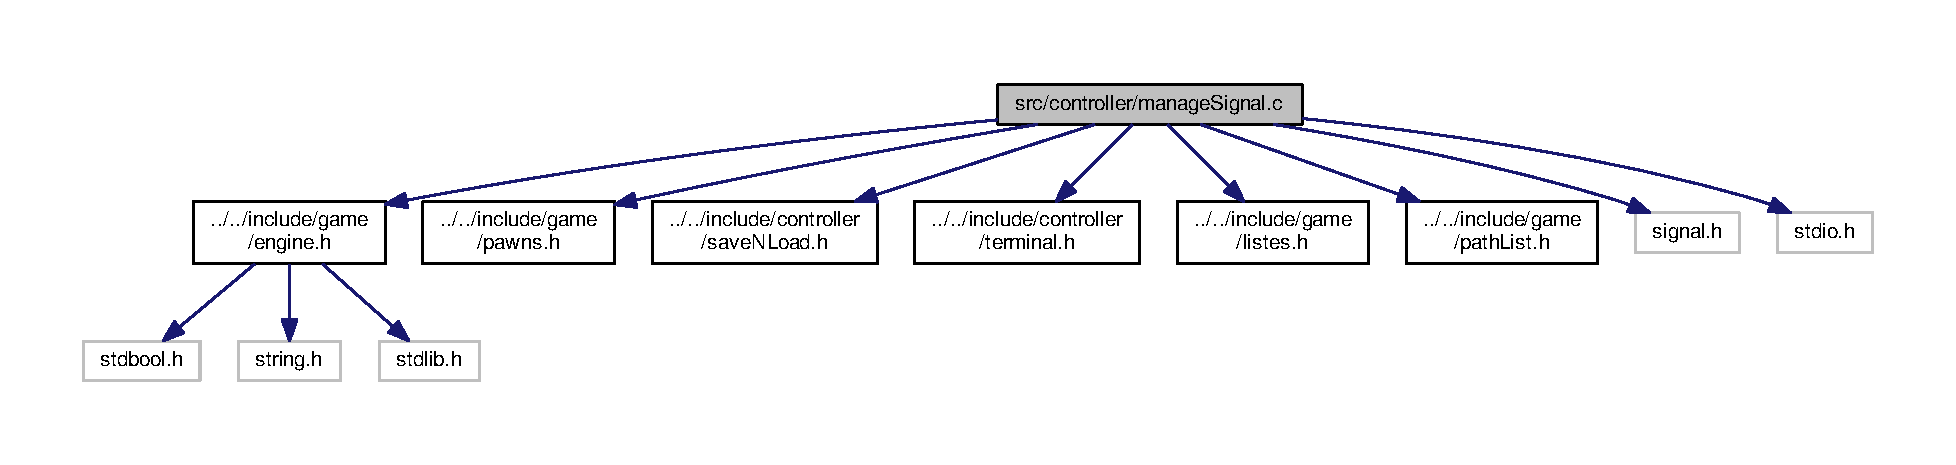
\includegraphics[width=350pt]{manageSignal_8c__incl}
\end{center}
\end{figure}
\subsection*{Fonctions}
\begin{DoxyCompactItemize}
\item 
void \hyperlink{manageSignal_8c_a91d6dcb4b4e4637a63aacf87b53132d0}{free\+All} ()
\begin{DoxyCompactList}\small\item\em Libère tout ce qui reste encore en mémoire. \end{DoxyCompactList}\item 
void \hyperlink{manageSignal_8c_a3e5752446c050a50659851e5f43fbc28}{interrupt} (int signal)
\begin{DoxyCompactList}\small\item\em A l\textquotesingle{}interruption du programme libère la mémoire et sauvegarde du jeu. \end{DoxyCompactList}\item 
void \hyperlink{manageSignal_8c_a04a93a7ee658050301abb6c4678c8923}{time\+Down} (int signal)
\begin{DoxyCompactList}\small\item\em Petit message sympa lors du temps écoulé \end{DoxyCompactList}\item 
void \hyperlink{manageSignal_8c_ab3fc6b27b6df879a96d8534e924139c4}{terminator} (int signal)
\begin{DoxyCompactList}\small\item\em Libération de la mémoire lors de la fin du programme. \end{DoxyCompactList}\item 
void \hyperlink{manageSignal_8c_a977fba31c29f9467d31b3efb9e0f8706}{check\+Signal} ()
\begin{DoxyCompactList}\small\item\em Vérifie le type de signal envoyé au terminal. \end{DoxyCompactList}\end{DoxyCompactItemize}


\subsection{Description détaillée}
Gestion des signaux. 

\begin{DoxyAuthor}{Auteur}
Cousin Brandon Chaudemanche Ewen Biardeau Tristan 
\end{DoxyAuthor}
\begin{DoxyVersion}{Version}
v1.\+00 
\end{DoxyVersion}
\begin{DoxyDate}{Date}
18/12/2015 
\end{DoxyDate}


\subsection{Documentation des fonctions}
\hypertarget{manageSignal_8c_a977fba31c29f9467d31b3efb9e0f8706}{}\index{manage\+Signal.\+c@{manage\+Signal.\+c}!check\+Signal@{check\+Signal}}
\index{check\+Signal@{check\+Signal}!manage\+Signal.\+c@{manage\+Signal.\+c}}
\subsubsection[{check\+Signal}]{\setlength{\rightskip}{0pt plus 5cm}void check\+Signal (
\begin{DoxyParamCaption}
{}
\end{DoxyParamCaption}
)}\label{manageSignal_8c_a977fba31c29f9467d31b3efb9e0f8706}


Vérifie le type de signal envoyé au terminal. 

Vérifie les signaux du programme. 

Définition à la ligne 77 du fichier manage\+Signal.\+c.

\hypertarget{manageSignal_8c_a91d6dcb4b4e4637a63aacf87b53132d0}{}\index{manage\+Signal.\+c@{manage\+Signal.\+c}!free\+All@{free\+All}}
\index{free\+All@{free\+All}!manage\+Signal.\+c@{manage\+Signal.\+c}}
\subsubsection[{free\+All}]{\setlength{\rightskip}{0pt plus 5cm}void free\+All (
\begin{DoxyParamCaption}
{}
\end{DoxyParamCaption}
)}\label{manageSignal_8c_a91d6dcb4b4e4637a63aacf87b53132d0}


Libère tout ce qui reste encore en mémoire. 

Libère toute la mémoire. 

Définition à la ligne 21 du fichier manage\+Signal.\+c.

\hypertarget{manageSignal_8c_a3e5752446c050a50659851e5f43fbc28}{}\index{manage\+Signal.\+c@{manage\+Signal.\+c}!interrupt@{interrupt}}
\index{interrupt@{interrupt}!manage\+Signal.\+c@{manage\+Signal.\+c}}
\subsubsection[{interrupt}]{\setlength{\rightskip}{0pt plus 5cm}void interrupt (
\begin{DoxyParamCaption}
\item[{int}]{signal}
\end{DoxyParamCaption}
)}\label{manageSignal_8c_a3e5752446c050a50659851e5f43fbc28}


A l\textquotesingle{}interruption du programme libère la mémoire et sauvegarde du jeu. 


\begin{DoxyParams}{Paramètres}
{\em signal} & Signal d\textquotesingle{}interruption \\
\hline
\end{DoxyParams}


Définition à la ligne 35 du fichier manage\+Signal.\+c.

\hypertarget{manageSignal_8c_ab3fc6b27b6df879a96d8534e924139c4}{}\index{manage\+Signal.\+c@{manage\+Signal.\+c}!terminator@{terminator}}
\index{terminator@{terminator}!manage\+Signal.\+c@{manage\+Signal.\+c}}
\subsubsection[{terminator}]{\setlength{\rightskip}{0pt plus 5cm}void terminator (
\begin{DoxyParamCaption}
\item[{int}]{signal}
\end{DoxyParamCaption}
)}\label{manageSignal_8c_ab3fc6b27b6df879a96d8534e924139c4}


Libération de la mémoire lors de la fin du programme. 


\begin{DoxyParams}{Paramètres}
{\em signal} & Signal d\textquotesingle{}interruption \\
\hline
\end{DoxyParams}


Définition à la ligne 68 du fichier manage\+Signal.\+c.

\hypertarget{manageSignal_8c_a04a93a7ee658050301abb6c4678c8923}{}\index{manage\+Signal.\+c@{manage\+Signal.\+c}!time\+Down@{time\+Down}}
\index{time\+Down@{time\+Down}!manage\+Signal.\+c@{manage\+Signal.\+c}}
\subsubsection[{time\+Down}]{\setlength{\rightskip}{0pt plus 5cm}void time\+Down (
\begin{DoxyParamCaption}
\item[{int}]{signal}
\end{DoxyParamCaption}
)}\label{manageSignal_8c_a04a93a7ee658050301abb6c4678c8923}


Petit message sympa lors du temps écoulé 


\begin{DoxyParams}{Paramètres}
{\em signal} & Signal d\textquotesingle{}interruption \\
\hline
\end{DoxyParams}


Définition à la ligne 58 du fichier manage\+Signal.\+c.


\hypertarget{manageString_8c}{}\section{Référence du fichier src/controller/manage\+String.c}
\label{manageString_8c}\index{src/controller/manage\+String.\+c@{src/controller/manage\+String.\+c}}


Gestions des chaînes de caractères.  


{\ttfamily \#include $<$ctype.\+h$>$}\\*
{\ttfamily \#include $<$stdio.\+h$>$}\\*
{\ttfamily \#include \char`\"{}../../include/game/engine.\+h\char`\"{}}\\*
Graphe des dépendances par inclusion de manage\+String.\+c\+:\nopagebreak
\begin{figure}[H]
\begin{center}
\leavevmode
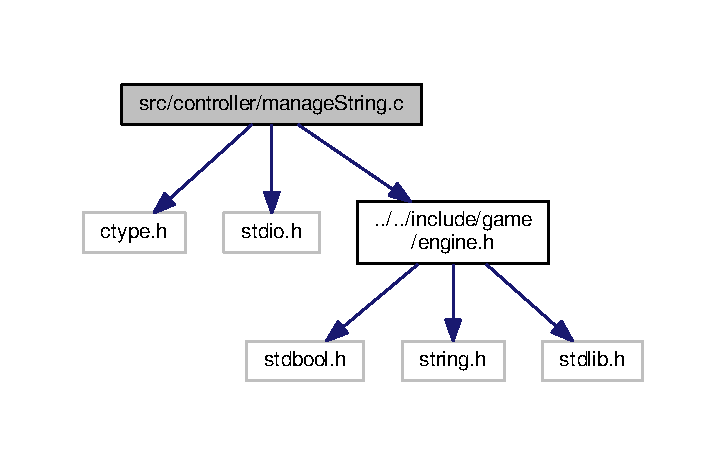
\includegraphics[width=349pt]{manageString_8c__incl}
\end{center}
\end{figure}
\subsection*{Fonctions}
\begin{DoxyCompactItemize}
\item 
void \hyperlink{manageString_8c_a4660decf36a299266867a3fdffd4891f}{get\+Coord\+S} (char coord\+String\mbox{[}$\,$\mbox{]}, \hyperlink{structvector}{vector} $\ast$coord\+Unit)
\begin{DoxyCompactList}\small\item\em Récupère les coordonnées d\textquotesingle{}une chaîne de caractère sous forme de vecteur x et y. \end{DoxyCompactList}\item 
char $\ast$ \hyperlink{manageString_8c_aef4f9d954282d13b5ea3132465378b79}{get2\+Char} (char name\mbox{[}$\,$\mbox{]})
\begin{DoxyCompactList}\small\item\em Récupère 2 caractères du nom de l\textquotesingle{}unité \end{DoxyCompactList}\item 
bool \hyperlink{manageString_8c_a65ed5e5cca1d9f5a66a56e36fc61dfcf}{is\+Out\+Grid} (char coord\+String\mbox{[}$\,$\mbox{]})
\begin{DoxyCompactList}\small\item\em Vérifie que les coordonnées sont dans la grille. \end{DoxyCompactList}\item 
bool \hyperlink{manageString_8c_a89a9fa2c469e9a139bff745dc48aeab7}{correct\+Coord} (char coord\+String\mbox{[}$\,$\mbox{]})
\begin{DoxyCompactList}\small\item\em Sélectionne une coordonnée et vérifie son format. \end{DoxyCompactList}\item 
bool \hyperlink{manageString_8c_a56a4267e397f3c206d9655b52241024e}{right\+Side} (char $\ast$coord\+String)
\begin{DoxyCompactList}\small\item\em Vérifie que l\textquotesingle{}unité est du bon côté \end{DoxyCompactList}\item 
char $\ast$ \hyperlink{manageString_8c_a22a30b59c6429cb81fcd18b4db5a1b7f}{get\+Name\+Unit} (\hyperlink{engine_8h_af7667555c2dcfbdd55ec3e9dd6a907ba}{unit\+Name} name)
\begin{DoxyCompactList}\small\item\em Récupère le nom de l\textquotesingle{}unité à partir de la liste énumérée. \end{DoxyCompactList}\item 
char $\ast$ \hyperlink{manageString_8c_acb5c8162f1db822caca54e0e04d2a143}{get\+Name\+Effect} (\hyperlink{engine_8h_ac5ece9b6993cd3565502866b56317e84}{unit\+Effect} effect)
\begin{DoxyCompactList}\small\item\em Récupère le nom de l\textquotesingle{}effet à partir de la liste énumérée. \end{DoxyCompactList}\item 
char $\ast$ \hyperlink{manageString_8c_a71644b2a2c56b83debb3c804040d3c88}{get\+Direction\+Unit} (\hyperlink{engine_8h_a468af3d7606639780e81c5e1e403b356}{cardinal} direct)
\begin{DoxyCompactList}\small\item\em Retourne la direction. \end{DoxyCompactList}\item 
void \hyperlink{manageString_8c_a32a341ce2c2a9240c500f694c9227b96}{print\+Name\+Unit} (\hyperlink{engine_8h_af7667555c2dcfbdd55ec3e9dd6a907ba}{unit\+Name} \hyperlink{structunit}{unit})
\begin{DoxyCompactList}\small\item\em Affiche le nom de l\textquotesingle{}unité \end{DoxyCompactList}\item 
void \hyperlink{manageString_8c_a20bbd4d45e3f01305dd709f5a9cc9952}{clear\+Buffer} ()
\begin{DoxyCompactList}\small\item\em Vide le tampon mémoire. \end{DoxyCompactList}\item 
int \hyperlink{manageString_8c_a57860307a2f1d8a80d71147a7ed1b793}{read\+S} (char $\ast$string)
\begin{DoxyCompactList}\small\item\em Lit la chaîne de caractère passée en paramètre et vérifie qu\textquotesingle{}elle ne soit pas trop longue. \end{DoxyCompactList}\item 
long \hyperlink{manageString_8c_ab431b0689298bfb6b1e74cbe92c18e00}{read\+Long} ()
\begin{DoxyCompactList}\small\item\em Lit un long de manière sécurisée. \end{DoxyCompactList}\item 
double \hyperlink{manageString_8c_a840ea5c01770156bd51bdb9f65f44e30}{read\+Double} ()
\begin{DoxyCompactList}\small\item\em Lit un double de manière sécurisée. \end{DoxyCompactList}\end{DoxyCompactItemize}


\subsection{Description détaillée}
Gestions des chaînes de caractères. 

\begin{DoxyAuthor}{Auteur}
Cousin Brandon Chaudemanche Ewen Biardeau Tristan 
\end{DoxyAuthor}
\begin{DoxyVersion}{Version}
v1.\+00 
\end{DoxyVersion}
\begin{DoxyDate}{Date}
18/12/2015 
\end{DoxyDate}


\subsection{Documentation des fonctions}
\hypertarget{manageString_8c_a20bbd4d45e3f01305dd709f5a9cc9952}{}\index{manage\+String.\+c@{manage\+String.\+c}!clear\+Buffer@{clear\+Buffer}}
\index{clear\+Buffer@{clear\+Buffer}!manage\+String.\+c@{manage\+String.\+c}}
\subsubsection[{clear\+Buffer}]{\setlength{\rightskip}{0pt plus 5cm}void clear\+Buffer (
\begin{DoxyParamCaption}
{}
\end{DoxyParamCaption}
)}\label{manageString_8c_a20bbd4d45e3f01305dd709f5a9cc9952}


Vide le tampon mémoire. 

Vide la mémoire tampon. 

Définition à la ligne 253 du fichier manage\+String.\+c.

\hypertarget{manageString_8c_a89a9fa2c469e9a139bff745dc48aeab7}{}\index{manage\+String.\+c@{manage\+String.\+c}!correct\+Coord@{correct\+Coord}}
\index{correct\+Coord@{correct\+Coord}!manage\+String.\+c@{manage\+String.\+c}}
\subsubsection[{correct\+Coord}]{\setlength{\rightskip}{0pt plus 5cm}bool correct\+Coord (
\begin{DoxyParamCaption}
\item[{char}]{coord\+String\mbox{[}$\,$\mbox{]}}
\end{DoxyParamCaption}
)}\label{manageString_8c_a89a9fa2c469e9a139bff745dc48aeab7}


Sélectionne une coordonnée et vérifie son format. 


\begin{DoxyParams}{Paramètres}
{\em coord\+String} & Chaîne de caractère à vérifier \\
\hline
\end{DoxyParams}
\begin{DoxyReturn}{Renvoie}
Vraie si les coordonnées saisies sont correctes 
\end{DoxyReturn}


Définition à la ligne 138 du fichier manage\+String.\+c.

\hypertarget{manageString_8c_aef4f9d954282d13b5ea3132465378b79}{}\index{manage\+String.\+c@{manage\+String.\+c}!get2\+Char@{get2\+Char}}
\index{get2\+Char@{get2\+Char}!manage\+String.\+c@{manage\+String.\+c}}
\subsubsection[{get2\+Char}]{\setlength{\rightskip}{0pt plus 5cm}char$\ast$ get2\+Char (
\begin{DoxyParamCaption}
\item[{char}]{name\mbox{[}$\,$\mbox{]}}
\end{DoxyParamCaption}
)}\label{manageString_8c_aef4f9d954282d13b5ea3132465378b79}


Récupère 2 caractères du nom de l\textquotesingle{}unité 


\begin{DoxyParams}{Paramètres}
{\em name} & Nom de l\textquotesingle{}unité \\
\hline
\end{DoxyParams}
\begin{DoxyReturn}{Renvoie}
Retourne 2 caractères liés au nom de l\textquotesingle{}unité 
\end{DoxyReturn}


Définition à la ligne 47 du fichier manage\+String.\+c.

\hypertarget{manageString_8c_a4660decf36a299266867a3fdffd4891f}{}\index{manage\+String.\+c@{manage\+String.\+c}!get\+Coord\+S@{get\+Coord\+S}}
\index{get\+Coord\+S@{get\+Coord\+S}!manage\+String.\+c@{manage\+String.\+c}}
\subsubsection[{get\+Coord\+S}]{\setlength{\rightskip}{0pt plus 5cm}void get\+Coord\+S (
\begin{DoxyParamCaption}
\item[{char}]{coord\+String\mbox{[}$\,$\mbox{]}, }
\item[{{\bf vector} $\ast$}]{coord\+Unit}
\end{DoxyParamCaption}
)}\label{manageString_8c_a4660decf36a299266867a3fdffd4891f}


Récupère les coordonnées d\textquotesingle{}une chaîne de caractère sous forme de vecteur x et y. 

Récupère les coordonnées d\textquotesingle{}une chaîne de caractères.


\begin{DoxyParams}{Paramètres}
{\em coord\+String} & Coordonnées saisie par l\textquotesingle{}utilisateur \\
\hline
{\em coord\+Unit} & Coordonnées de l\textquotesingle{}unité récupérées de la saisie utilisateur \\
\hline
\end{DoxyParams}


Définition à la ligne 19 du fichier manage\+String.\+c.

\hypertarget{manageString_8c_a71644b2a2c56b83debb3c804040d3c88}{}\index{manage\+String.\+c@{manage\+String.\+c}!get\+Direction\+Unit@{get\+Direction\+Unit}}
\index{get\+Direction\+Unit@{get\+Direction\+Unit}!manage\+String.\+c@{manage\+String.\+c}}
\subsubsection[{get\+Direction\+Unit}]{\setlength{\rightskip}{0pt plus 5cm}char$\ast$ get\+Direction\+Unit (
\begin{DoxyParamCaption}
\item[{{\bf cardinal}}]{direct}
\end{DoxyParamCaption}
)}\label{manageString_8c_a71644b2a2c56b83debb3c804040d3c88}


Retourne la direction. 

Récupère le nom de la direction.


\begin{DoxyParams}{Paramètres}
{\em direct} & Direction de l\textquotesingle{}unité \\
\hline
\end{DoxyParams}
\begin{DoxyReturn}{Renvoie}
Retourne La direction sous forme de chaîne 
\end{DoxyReturn}


Définition à la ligne 235 du fichier manage\+String.\+c.

\hypertarget{manageString_8c_acb5c8162f1db822caca54e0e04d2a143}{}\index{manage\+String.\+c@{manage\+String.\+c}!get\+Name\+Effect@{get\+Name\+Effect}}
\index{get\+Name\+Effect@{get\+Name\+Effect}!manage\+String.\+c@{manage\+String.\+c}}
\subsubsection[{get\+Name\+Effect}]{\setlength{\rightskip}{0pt plus 5cm}char$\ast$ get\+Name\+Effect (
\begin{DoxyParamCaption}
\item[{{\bf unit\+Effect}}]{effect}
\end{DoxyParamCaption}
)}\label{manageString_8c_acb5c8162f1db822caca54e0e04d2a143}


Récupère le nom de l\textquotesingle{}effet à partir de la liste énumérée. 

Récupère le nom de l\textquotesingle{}effet.


\begin{DoxyParams}{Paramètres}
{\em effect} & Effet provenant de la liste énumérée \\
\hline
\end{DoxyParams}
\begin{DoxyReturn}{Renvoie}
Nom de l\textquotesingle{}effet sous forme de chaîne de caractère 
\end{DoxyReturn}


Définition à la ligne 220 du fichier manage\+String.\+c.

\hypertarget{manageString_8c_a22a30b59c6429cb81fcd18b4db5a1b7f}{}\index{manage\+String.\+c@{manage\+String.\+c}!get\+Name\+Unit@{get\+Name\+Unit}}
\index{get\+Name\+Unit@{get\+Name\+Unit}!manage\+String.\+c@{manage\+String.\+c}}
\subsubsection[{get\+Name\+Unit}]{\setlength{\rightskip}{0pt plus 5cm}char$\ast$ get\+Name\+Unit (
\begin{DoxyParamCaption}
\item[{{\bf unit\+Name}}]{name}
\end{DoxyParamCaption}
)}\label{manageString_8c_a22a30b59c6429cb81fcd18b4db5a1b7f}


Récupère le nom de l\textquotesingle{}unité à partir de la liste énumérée. 

Récupère le nom de l\textquotesingle{}unité


\begin{DoxyParams}{Paramètres}
{\em name} & Nom de l\textquotesingle{}unité provenant de la liste énumérée \\
\hline
\end{DoxyParams}
\begin{DoxyReturn}{Renvoie}
Nom de l\textquotesingle{}unité sous forme de chaîne 
\end{DoxyReturn}


Définition à la ligne 189 du fichier manage\+String.\+c.

\hypertarget{manageString_8c_a65ed5e5cca1d9f5a66a56e36fc61dfcf}{}\index{manage\+String.\+c@{manage\+String.\+c}!is\+Out\+Grid@{is\+Out\+Grid}}
\index{is\+Out\+Grid@{is\+Out\+Grid}!manage\+String.\+c@{manage\+String.\+c}}
\subsubsection[{is\+Out\+Grid}]{\setlength{\rightskip}{0pt plus 5cm}bool is\+Out\+Grid (
\begin{DoxyParamCaption}
\item[{char}]{coord\+String\mbox{[}$\,$\mbox{]}}
\end{DoxyParamCaption}
)}\label{manageString_8c_a65ed5e5cca1d9f5a66a56e36fc61dfcf}


Vérifie que les coordonnées sont dans la grille. 


\begin{DoxyParams}{Paramètres}
{\em coord\+String} & Coordonnées sous forme de chaîne \\
\hline
\end{DoxyParams}
\begin{DoxyReturn}{Renvoie}
Retourne false si pas en dehors 
\end{DoxyReturn}


Définition à la ligne 114 du fichier manage\+String.\+c.

\hypertarget{manageString_8c_a32a341ce2c2a9240c500f694c9227b96}{}\index{manage\+String.\+c@{manage\+String.\+c}!print\+Name\+Unit@{print\+Name\+Unit}}
\index{print\+Name\+Unit@{print\+Name\+Unit}!manage\+String.\+c@{manage\+String.\+c}}
\subsubsection[{print\+Name\+Unit}]{\setlength{\rightskip}{0pt plus 5cm}void print\+Name\+Unit (
\begin{DoxyParamCaption}
\item[{{\bf unit\+Name}}]{unit}
\end{DoxyParamCaption}
)}\label{manageString_8c_a32a341ce2c2a9240c500f694c9227b96}


Affiche le nom de l\textquotesingle{}unité 


\begin{DoxyParams}{Paramètres}
{\em unit} & Nom de l\textquotesingle{}unité provenant de la liste énumérée \\
\hline
\end{DoxyParams}


Définition à la ligne 246 du fichier manage\+String.\+c.

\hypertarget{manageString_8c_a840ea5c01770156bd51bdb9f65f44e30}{}\index{manage\+String.\+c@{manage\+String.\+c}!read\+Double@{read\+Double}}
\index{read\+Double@{read\+Double}!manage\+String.\+c@{manage\+String.\+c}}
\subsubsection[{read\+Double}]{\setlength{\rightskip}{0pt plus 5cm}double read\+Double (
\begin{DoxyParamCaption}
{}
\end{DoxyParamCaption}
)}\label{manageString_8c_a840ea5c01770156bd51bdb9f65f44e30}


Lit un double de manière sécurisée. 

Lecture sécurisée d\textquotesingle{}un double.

\begin{DoxyReturn}{Renvoie}
Retourne le double saisie ou 0.\+0 en cas d\textquotesingle{}erreur 
\end{DoxyReturn}


Définition à la ligne 305 du fichier manage\+String.\+c.

\hypertarget{manageString_8c_ab431b0689298bfb6b1e74cbe92c18e00}{}\index{manage\+String.\+c@{manage\+String.\+c}!read\+Long@{read\+Long}}
\index{read\+Long@{read\+Long}!manage\+String.\+c@{manage\+String.\+c}}
\subsubsection[{read\+Long}]{\setlength{\rightskip}{0pt plus 5cm}long read\+Long (
\begin{DoxyParamCaption}
{}
\end{DoxyParamCaption}
)}\label{manageString_8c_ab431b0689298bfb6b1e74cbe92c18e00}


Lit un long de manière sécurisée. 

Lecture sécurisée d\textquotesingle{}un long.

\begin{DoxyReturn}{Renvoie}
Retourne le long saisie ou 0 en cas d\textquotesingle{}erreur 
\end{DoxyReturn}


Définition à la ligne 291 du fichier manage\+String.\+c.

\hypertarget{manageString_8c_a57860307a2f1d8a80d71147a7ed1b793}{}\index{manage\+String.\+c@{manage\+String.\+c}!read\+S@{read\+S}}
\index{read\+S@{read\+S}!manage\+String.\+c@{manage\+String.\+c}}
\subsubsection[{read\+S}]{\setlength{\rightskip}{0pt plus 5cm}int read\+S (
\begin{DoxyParamCaption}
\item[{char $\ast$}]{string}
\end{DoxyParamCaption}
)}\label{manageString_8c_a57860307a2f1d8a80d71147a7ed1b793}


Lit la chaîne de caractère passée en paramètre et vérifie qu\textquotesingle{}elle ne soit pas trop longue. 

Lecture sécurisée d\textquotesingle{}une chaîne.


\begin{DoxyParams}{Paramètres}
{\em string} & Chaîne de caractère à vérifier \\
\hline
\end{DoxyParams}
\begin{DoxyReturn}{Renvoie}
Retourne 1 si chaîne correcte 
\end{DoxyReturn}


Définition à la ligne 265 du fichier manage\+String.\+c.

\hypertarget{manageString_8c_a56a4267e397f3c206d9655b52241024e}{}\index{manage\+String.\+c@{manage\+String.\+c}!right\+Side@{right\+Side}}
\index{right\+Side@{right\+Side}!manage\+String.\+c@{manage\+String.\+c}}
\subsubsection[{right\+Side}]{\setlength{\rightskip}{0pt plus 5cm}bool right\+Side (
\begin{DoxyParamCaption}
\item[{char $\ast$}]{coord\+String}
\end{DoxyParamCaption}
)}\label{manageString_8c_a56a4267e397f3c206d9655b52241024e}


Vérifie que l\textquotesingle{}unité est du bon côté 

Vérifie que l\textquotesingle{}unité est dans le bon camp.


\begin{DoxyParams}{Paramètres}
{\em coord\+String} & Coordonnées sous forme de chaîne \\
\hline
\end{DoxyParams}
\begin{DoxyReturn}{Renvoie}
Retourne vrai si du bon côté 
\end{DoxyReturn}


Définition à la ligne 165 du fichier manage\+String.\+c.


\hypertarget{saveNLoad_8c}{}\section{Référence du fichier src/controller/save\+N\+Load.c}
\label{saveNLoad_8c}\index{src/controller/save\+N\+Load.\+c@{src/controller/save\+N\+Load.\+c}}


Gestion de la sauvegarde et du chargement.  


{\ttfamily \#include $<$stdio.\+h$>$}\\*
{\ttfamily \#include \char`\"{}../../include/game/engine.\+h\char`\"{}}\\*
{\ttfamily \#include \char`\"{}../../include/game/pawns.\+h\char`\"{}}\\*
{\ttfamily \#include \char`\"{}../../include/game/listes.\+h\char`\"{}}\\*
{\ttfamily \#include \char`\"{}../../include/game/path\+List.\+h\char`\"{}}\\*
{\ttfamily \#include \char`\"{}../../include/game/turn.\+h\char`\"{}}\\*
{\ttfamily \#include \char`\"{}../../include/display/grid.\+h\char`\"{}}\\*
{\ttfamily \#include \char`\"{}../../include/controller/terminal.\+h\char`\"{}}\\*
{\ttfamily \#include \char`\"{}../../include/controller/manage\+String.\+h\char`\"{}}\\*
Graphe des dépendances par inclusion de save\+N\+Load.\+c\+:\nopagebreak
\begin{figure}[H]
\begin{center}
\leavevmode
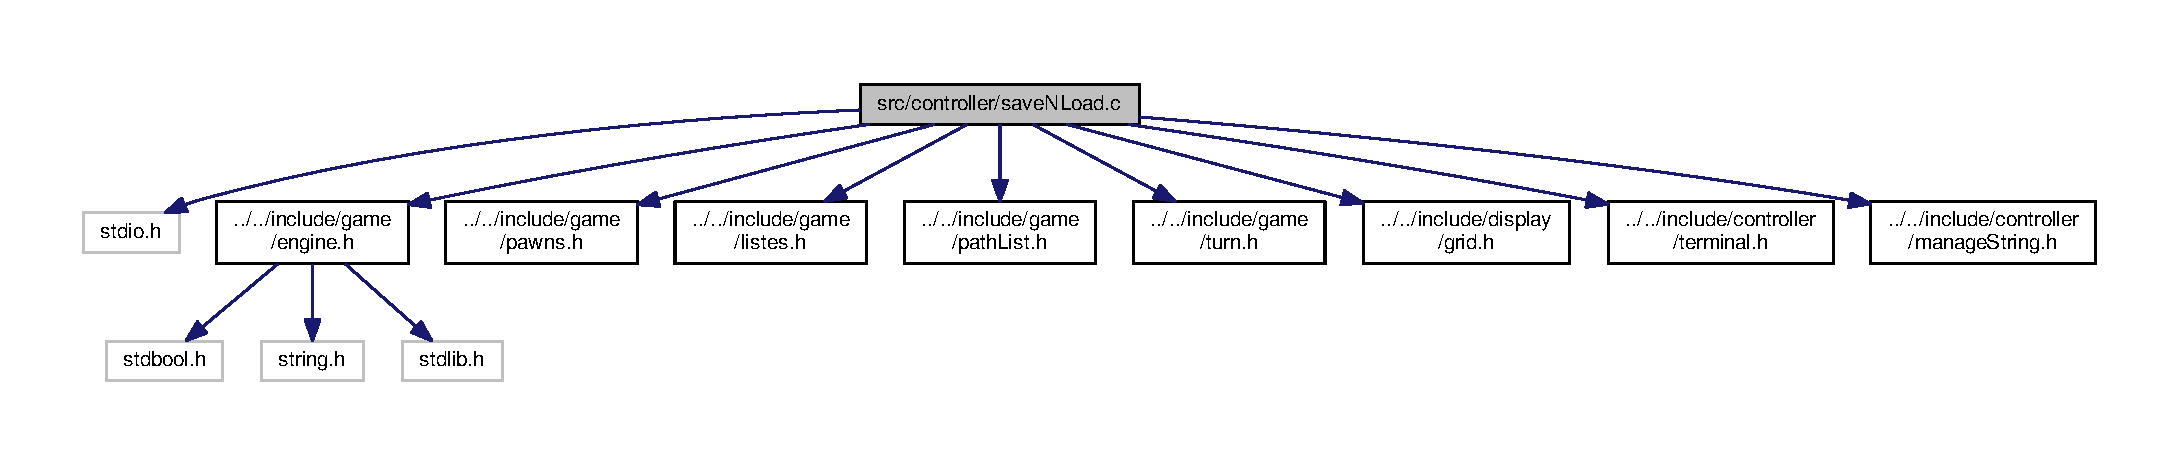
\includegraphics[width=350pt]{saveNLoad_8c__incl}
\end{center}
\end{figure}
\subsection*{Fonctions}
\begin{DoxyCompactItemize}
\item 
char \hyperlink{saveNLoad_8c_a6a1368e194a9e07bdd18d953515bb3f2}{get\+Char\+Key} (char $\ast$dynamic\+Key, int $\ast$pos)
\begin{DoxyCompactList}\small\item\em Récupère un caractère de la clé \end{DoxyCompactList}\item 
char $\ast$ \hyperlink{saveNLoad_8c_a7ec2efd1e49dcbbda52c7b31438f61ec}{get\+Key} (\hyperlink{engine_8h_af7667555c2dcfbdd55ec3e9dd6a907ba}{unit\+Name} name)
\begin{DoxyCompactList}\small\item\em Récupère une clé de décryptage. \end{DoxyCompactList}\item 
void \hyperlink{saveNLoad_8c_a1c3b7026831b763b387a0de575af10b4}{crypt} (\hyperlink{structunit}{unit} $\ast$unit\+Saved)
\begin{DoxyCompactList}\small\item\em Crypte les statistiques de l\textquotesingle{}unité pour la sauvegarde. \end{DoxyCompactList}\item 
void \hyperlink{saveNLoad_8c_a5d5052b4a62dde604172e0d8709026a2}{decrypt} (\hyperlink{structunit}{unit} $\ast$unit\+Loaded)
\begin{DoxyCompactList}\small\item\em Décrypte les statistiques de l\textquotesingle{}unité pour le chargement. \end{DoxyCompactList}\item 
bool \hyperlink{saveNLoad_8c_aca91b85990102e4dd58d8728b11cc035}{check\+Decrypt} (\hyperlink{structunit}{unit} $\ast$unit\+Loaded)
\begin{DoxyCompactList}\small\item\em Vérifie que le décryptage s\textquotesingle{}est bien passé \end{DoxyCompactList}\item 
void \hyperlink{saveNLoad_8c_aae2c382151ef7c9aa913361172b30db6}{save} ()
\begin{DoxyCompactList}\small\item\em Sauvegarde la partie avec l\textquotesingle{}état actuel de la grille et les données liées au joueur en cours. \end{DoxyCompactList}\item 
void \hyperlink{saveNLoad_8c_a78f61ac2dd03bcba8e09ca20cd7d68e3}{load} ()
\begin{DoxyCompactList}\small\item\em Charge la partie précédemment enregistré \end{DoxyCompactList}\end{DoxyCompactItemize}
\subsection*{Variables}
\begin{DoxyCompactItemize}
\item 
\hypertarget{saveNLoad_8c_a11a7310ee9d77476871dbe977e71a7f4}{}char \hyperlink{saveNLoad_8c_a11a7310ee9d77476871dbe977e71a7f4}{key} \mbox{[}$\,$\mbox{]} = \char`\"{}S\+P\+I\+B\+C\+T\+B\+E\+C\char`\"{}\label{saveNLoad_8c_a11a7310ee9d77476871dbe977e71a7f4}

\begin{DoxyCompactList}\small\item\em Clé statique à utiliser pour le cryptage. \end{DoxyCompactList}\end{DoxyCompactItemize}


\subsection{Description détaillée}
Gestion de la sauvegarde et du chargement. 

\begin{DoxyAuthor}{Auteur}
Cousin Brandon Chaudemanche Ewen Biardeau Tristan 
\end{DoxyAuthor}
\begin{DoxyVersion}{Version}
v1.\+00 
\end{DoxyVersion}
\begin{DoxyDate}{Date}
18/12/2015 
\end{DoxyDate}


\subsection{Documentation des fonctions}
\hypertarget{saveNLoad_8c_aca91b85990102e4dd58d8728b11cc035}{}\index{save\+N\+Load.\+c@{save\+N\+Load.\+c}!check\+Decrypt@{check\+Decrypt}}
\index{check\+Decrypt@{check\+Decrypt}!save\+N\+Load.\+c@{save\+N\+Load.\+c}}
\subsubsection[{check\+Decrypt}]{\setlength{\rightskip}{0pt plus 5cm}bool check\+Decrypt (
\begin{DoxyParamCaption}
\item[{{\bf unit} $\ast$}]{unit\+Loaded}
\end{DoxyParamCaption}
)}\label{saveNLoad_8c_aca91b85990102e4dd58d8728b11cc035}


Vérifie que le décryptage s\textquotesingle{}est bien passé 


\begin{DoxyParams}{Paramètres}
{\em unit\+Loaded} & Unité chargée \\
\hline
\end{DoxyParams}
\begin{DoxyReturn}{Renvoie}
Retourne vrai si données correctes sinon faux 
\end{DoxyReturn}


Définition à la ligne 133 du fichier save\+N\+Load.\+c.

\hypertarget{saveNLoad_8c_a1c3b7026831b763b387a0de575af10b4}{}\index{save\+N\+Load.\+c@{save\+N\+Load.\+c}!crypt@{crypt}}
\index{crypt@{crypt}!save\+N\+Load.\+c@{save\+N\+Load.\+c}}
\subsubsection[{crypt}]{\setlength{\rightskip}{0pt plus 5cm}void crypt (
\begin{DoxyParamCaption}
\item[{{\bf unit} $\ast$}]{unit\+Saved}
\end{DoxyParamCaption}
)}\label{saveNLoad_8c_a1c3b7026831b763b387a0de575af10b4}


Crypte les statistiques de l\textquotesingle{}unité pour la sauvegarde. 


\begin{DoxyParams}{Paramètres}
{\em unit\+Saved} & Unité sauvegardée \\
\hline
\end{DoxyParams}


Définition à la ligne 70 du fichier save\+N\+Load.\+c.

\hypertarget{saveNLoad_8c_a5d5052b4a62dde604172e0d8709026a2}{}\index{save\+N\+Load.\+c@{save\+N\+Load.\+c}!decrypt@{decrypt}}
\index{decrypt@{decrypt}!save\+N\+Load.\+c@{save\+N\+Load.\+c}}
\subsubsection[{decrypt}]{\setlength{\rightskip}{0pt plus 5cm}void decrypt (
\begin{DoxyParamCaption}
\item[{{\bf unit} $\ast$}]{unit\+Loaded}
\end{DoxyParamCaption}
)}\label{saveNLoad_8c_a5d5052b4a62dde604172e0d8709026a2}


Décrypte les statistiques de l\textquotesingle{}unité pour le chargement. 


\begin{DoxyParams}{Paramètres}
{\em unit\+Loaded} & Unité chargée \\
\hline
\end{DoxyParams}


Définition à la ligne 101 du fichier save\+N\+Load.\+c.

\hypertarget{saveNLoad_8c_a6a1368e194a9e07bdd18d953515bb3f2}{}\index{save\+N\+Load.\+c@{save\+N\+Load.\+c}!get\+Char\+Key@{get\+Char\+Key}}
\index{get\+Char\+Key@{get\+Char\+Key}!save\+N\+Load.\+c@{save\+N\+Load.\+c}}
\subsubsection[{get\+Char\+Key}]{\setlength{\rightskip}{0pt plus 5cm}char get\+Char\+Key (
\begin{DoxyParamCaption}
\item[{char $\ast$}]{dynamic\+Key, }
\item[{int $\ast$}]{pos}
\end{DoxyParamCaption}
)}\label{saveNLoad_8c_a6a1368e194a9e07bdd18d953515bb3f2}


Récupère un caractère de la clé 


\begin{DoxyParams}{Paramètres}
{\em dynamic\+Key} & Clé dynamique \\
\hline
{\em pos} & Position dans la clé \\
\hline
\end{DoxyParams}
\begin{DoxyReturn}{Renvoie}
Retourne un caractère de la clé 
\end{DoxyReturn}


Définition à la ligne 27 du fichier save\+N\+Load.\+c.

\hypertarget{saveNLoad_8c_a7ec2efd1e49dcbbda52c7b31438f61ec}{}\index{save\+N\+Load.\+c@{save\+N\+Load.\+c}!get\+Key@{get\+Key}}
\index{get\+Key@{get\+Key}!save\+N\+Load.\+c@{save\+N\+Load.\+c}}
\subsubsection[{get\+Key}]{\setlength{\rightskip}{0pt plus 5cm}char$\ast$ get\+Key (
\begin{DoxyParamCaption}
\item[{{\bf unit\+Name}}]{name}
\end{DoxyParamCaption}
)}\label{saveNLoad_8c_a7ec2efd1e49dcbbda52c7b31438f61ec}


Récupère une clé de décryptage. 


\begin{DoxyParams}{Paramètres}
{\em name} & Nom de l\textquotesingle{}unité \\
\hline
\end{DoxyParams}
\begin{DoxyReturn}{Renvoie}
Retourne une clé 
\end{DoxyReturn}


Définition à la ligne 39 du fichier save\+N\+Load.\+c.

\hypertarget{saveNLoad_8c_a78f61ac2dd03bcba8e09ca20cd7d68e3}{}\index{save\+N\+Load.\+c@{save\+N\+Load.\+c}!load@{load}}
\index{load@{load}!save\+N\+Load.\+c@{save\+N\+Load.\+c}}
\subsubsection[{load}]{\setlength{\rightskip}{0pt plus 5cm}void load (
\begin{DoxyParamCaption}
{}
\end{DoxyParamCaption}
)}\label{saveNLoad_8c_a78f61ac2dd03bcba8e09ca20cd7d68e3}


Charge la partie précédemment enregistré 

Charge une partie. 

Définition à la ligne 201 du fichier save\+N\+Load.\+c.

\hypertarget{saveNLoad_8c_aae2c382151ef7c9aa913361172b30db6}{}\index{save\+N\+Load.\+c@{save\+N\+Load.\+c}!save@{save}}
\index{save@{save}!save\+N\+Load.\+c@{save\+N\+Load.\+c}}
\subsubsection[{save}]{\setlength{\rightskip}{0pt plus 5cm}void save (
\begin{DoxyParamCaption}
{}
\end{DoxyParamCaption}
)}\label{saveNLoad_8c_aae2c382151ef7c9aa913361172b30db6}


Sauvegarde la partie avec l\textquotesingle{}état actuel de la grille et les données liées au joueur en cours. 

Sauvegarde la partie. 

Définition à la ligne 158 du fichier save\+N\+Load.\+c.


\hypertarget{terminal_8c}{}\section{Référence du fichier src/controller/terminal.c}
\label{terminal_8c}\index{src/controller/terminal.\+c@{src/controller/terminal.\+c}}


Gestion du terminal.  


{\ttfamily \#include $<$string.\+h$>$}\\*
{\ttfamily \#include $<$stdlib.\+h$>$}\\*
{\ttfamily \#include $<$stdio.\+h$>$}\\*
{\ttfamily \#include \char`\"{}../../include/controller/terminal.\+h\char`\"{}}\\*
{\ttfamily \#include \char`\"{}../../include/game/engine.\+h\char`\"{}}\\*
Graphe des dépendances par inclusion de terminal.\+c\+:\nopagebreak
\begin{figure}[H]
\begin{center}
\leavevmode
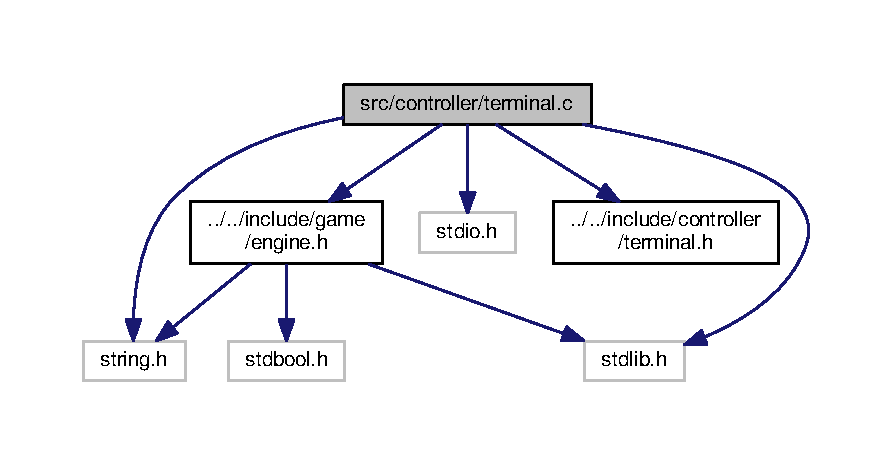
\includegraphics[width=350pt]{terminal_8c__incl}
\end{center}
\end{figure}
\subsection*{Fonctions}
\begin{DoxyCompactItemize}
\item 
char $\ast$ \hyperlink{terminal_8c_a27b5a8154971e29605c7c361c328263c}{get\+Color} (int \hyperlink{terminal_8h_aa1b198e2a86cf333bd2b8d74e21409f1}{color}, char type\mbox{[}$\,$\mbox{]})
\begin{DoxyCompactList}\small\item\em Récupère le code correspondant à la couleur. \end{DoxyCompactList}\item 
void \hyperlink{terminal_8c_aa1b198e2a86cf333bd2b8d74e21409f1}{color} (int color, char type\mbox{[}$\,$\mbox{]})
\begin{DoxyCompactList}\small\item\em Change la couleur de l\textquotesingle{}écran ou de la police. \end{DoxyCompactList}\item 
void \hyperlink{terminal_8c_aafe20dae78dfbeea7c9102fadcfba1e0}{reinit\+Color} ()
\begin{DoxyCompactList}\small\item\em Réinitialise la couleur de l\textquotesingle{}écran. \end{DoxyCompactList}\item 
void \hyperlink{terminal_8c_a728c5deabcb9e271c6962577c60ef566}{font\+Color} (int \hyperlink{terminal_8h_aa1b198e2a86cf333bd2b8d74e21409f1}{color})
\begin{DoxyCompactList}\small\item\em Change la couleur de la police. \end{DoxyCompactList}\item 
\hypertarget{terminal_8c_a9d7e8af417b6d543da691e9c0e2f6f9f}{}void \hyperlink{terminal_8c_a9d7e8af417b6d543da691e9c0e2f6f9f}{clear\+Screen} ()\label{terminal_8c_a9d7e8af417b6d543da691e9c0e2f6f9f}

\begin{DoxyCompactList}\small\item\em Efface l\textquotesingle{}écran. \end{DoxyCompactList}\end{DoxyCompactItemize}


\subsection{Description détaillée}
Gestion du terminal. 

\begin{DoxyAuthor}{Auteur}
Cousin Brandon Chaudemanche Ewen Biardeau Tristan 
\end{DoxyAuthor}
\begin{DoxyVersion}{Version}
v1.\+00 
\end{DoxyVersion}
\begin{DoxyDate}{Date}
18/12/2015 
\end{DoxyDate}


\subsection{Documentation des fonctions}
\hypertarget{terminal_8c_aa1b198e2a86cf333bd2b8d74e21409f1}{}\index{terminal.\+c@{terminal.\+c}!color@{color}}
\index{color@{color}!terminal.\+c@{terminal.\+c}}
\subsubsection[{color}]{\setlength{\rightskip}{0pt plus 5cm}void color (
\begin{DoxyParamCaption}
\item[{int}]{color, }
\item[{char}]{type\mbox{[}$\,$\mbox{]}}
\end{DoxyParamCaption}
)}\label{terminal_8c_aa1b198e2a86cf333bd2b8d74e21409f1}


Change la couleur de l\textquotesingle{}écran ou de la police. 

Met en couleurs le texte ou l\textquotesingle{}écran.


\begin{DoxyParams}{Paramètres}
{\em color} & Couleur à utiliser \\
\hline
{\em type} & Texte à changer de couleur ou arrière plan \\
\hline
\end{DoxyParams}


Définition à la ligne 51 du fichier terminal.\+c.

\hypertarget{terminal_8c_a728c5deabcb9e271c6962577c60ef566}{}\index{terminal.\+c@{terminal.\+c}!font\+Color@{font\+Color}}
\index{font\+Color@{font\+Color}!terminal.\+c@{terminal.\+c}}
\subsubsection[{font\+Color}]{\setlength{\rightskip}{0pt plus 5cm}void font\+Color (
\begin{DoxyParamCaption}
\item[{int}]{color}
\end{DoxyParamCaption}
)}\label{terminal_8c_a728c5deabcb9e271c6962577c60ef566}


Change la couleur de la police. 

Met en couleurs la police.


\begin{DoxyParams}{Paramètres}
{\em color} & Couleur à utiliser \\
\hline
\end{DoxyParams}


Définition à la ligne 76 du fichier terminal.\+c.

\hypertarget{terminal_8c_a27b5a8154971e29605c7c361c328263c}{}\index{terminal.\+c@{terminal.\+c}!get\+Color@{get\+Color}}
\index{get\+Color@{get\+Color}!terminal.\+c@{terminal.\+c}}
\subsubsection[{get\+Color}]{\setlength{\rightskip}{0pt plus 5cm}char$\ast$ get\+Color (
\begin{DoxyParamCaption}
\item[{int}]{color, }
\item[{char}]{type\mbox{[}$\,$\mbox{]}}
\end{DoxyParamCaption}
)}\label{terminal_8c_a27b5a8154971e29605c7c361c328263c}


Récupère le code correspondant à la couleur. 


\begin{DoxyParams}{Paramètres}
{\em color} & Couleur demandée \\
\hline
{\em type} & Type d\textquotesingle{}objet à modifier \\
\hline
\end{DoxyParams}
\begin{DoxyReturn}{Renvoie}
Code correspondant, écran blanc si code incorrect 
\end{DoxyReturn}


Définition à la ligne 21 du fichier terminal.\+c.

\hypertarget{terminal_8c_aafe20dae78dfbeea7c9102fadcfba1e0}{}\index{terminal.\+c@{terminal.\+c}!reinit\+Color@{reinit\+Color}}
\index{reinit\+Color@{reinit\+Color}!terminal.\+c@{terminal.\+c}}
\subsubsection[{reinit\+Color}]{\setlength{\rightskip}{0pt plus 5cm}void reinit\+Color (
\begin{DoxyParamCaption}
{}
\end{DoxyParamCaption}
)}\label{terminal_8c_aafe20dae78dfbeea7c9102fadcfba1e0}


Réinitialise la couleur de l\textquotesingle{}écran. 

Réinitialise les couleurs. 

Définition à la ligne 67 du fichier terminal.\+c.


\hypertarget{grid_8c}{}\section{Référence du fichier src/display/grid.c}
\label{grid_8c}\index{src/display/grid.\+c@{src/display/grid.\+c}}


Gestion de la grille.  


{\ttfamily \#include $<$stdio.\+h$>$}\\*
{\ttfamily \#include \char`\"{}../../include/game/engine.\+h\char`\"{}}\\*
{\ttfamily \#include \char`\"{}../../include/display/grid.\+h\char`\"{}}\\*
{\ttfamily \#include \char`\"{}../../include/controller/terminal.\+h\char`\"{}}\\*
{\ttfamily \#include \char`\"{}../../include/controller/manage\+String.\+h\char`\"{}}\\*
Graphe des dépendances par inclusion de grid.\+c\+:\nopagebreak
\begin{figure}[H]
\begin{center}
\leavevmode
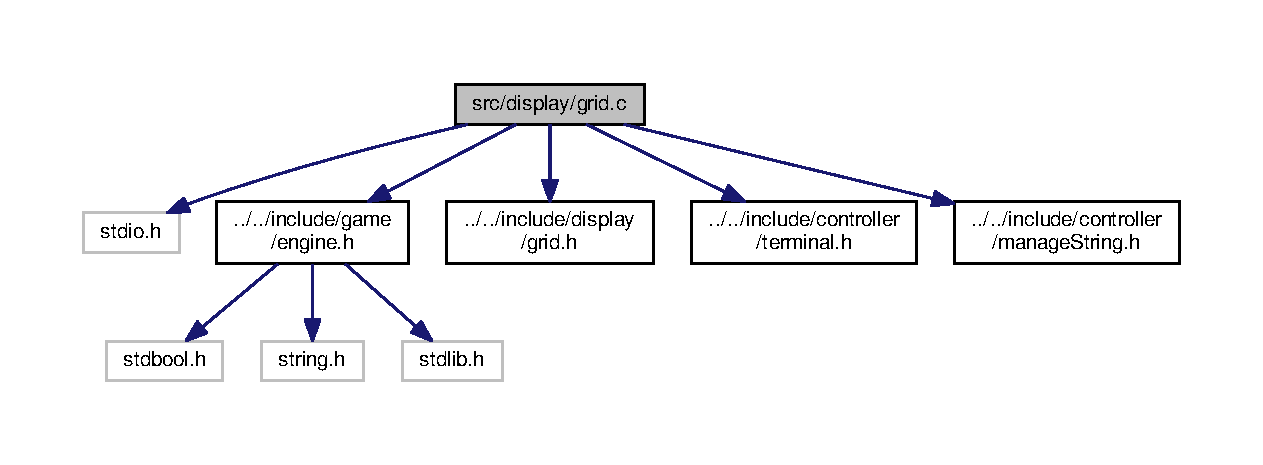
\includegraphics[width=350pt]{grid_8c__incl}
\end{center}
\end{figure}
\subsection*{Fonctions}
\begin{DoxyCompactItemize}
\item 
void \hyperlink{grid_8c_a1095651c2e5f692fd90166792ad43e7c}{border\+Right} (short row)
\begin{DoxyCompactList}\small\item\em Affiche une bordure sur le côté droit sur les lignes vides et utiles. \end{DoxyCompactList}\item 
\hypertarget{grid_8c_ace8aa29526b144ad331180783a7499cc}{}void \hyperlink{grid_8c_ace8aa29526b144ad331180783a7499cc}{border\+Horiz} ()\label{grid_8c_ace8aa29526b144ad331180783a7499cc}

\begin{DoxyCompactList}\small\item\em Affiche une bordure horizontale. \end{DoxyCompactList}\item 
\hypertarget{grid_8c_a5885768a9129c1301da1a5691ec5a830}{}void \hyperlink{grid_8c_a5885768a9129c1301da1a5691ec5a830}{disp\+X} ()\label{grid_8c_a5885768a9129c1301da1a5691ec5a830}

\begin{DoxyCompactList}\small\item\em Affiche les coordonnées verticales. \end{DoxyCompactList}\item 
void \hyperlink{grid_8c_aad3077ff809cfe68afdb06ef3aa5497f}{grid\+Disp} ()
\begin{DoxyCompactList}\small\item\em Affiche la grille avec les coordonnées. \end{DoxyCompactList}\end{DoxyCompactItemize}


\subsection{Description détaillée}
Gestion de la grille. 

\begin{DoxyAuthor}{Auteur}
Cousin Brandon Chaudemanche Ewen Biardeau Tristan 
\end{DoxyAuthor}
\begin{DoxyVersion}{Version}
v1.\+00 
\end{DoxyVersion}
\begin{DoxyDate}{Date}
18/12/2015 
\end{DoxyDate}


\subsection{Documentation des fonctions}
\hypertarget{grid_8c_a1095651c2e5f692fd90166792ad43e7c}{}\index{grid.\+c@{grid.\+c}!border\+Right@{border\+Right}}
\index{border\+Right@{border\+Right}!grid.\+c@{grid.\+c}}
\subsubsection[{border\+Right}]{\setlength{\rightskip}{0pt plus 5cm}void border\+Right (
\begin{DoxyParamCaption}
\item[{short}]{row}
\end{DoxyParamCaption}
)}\label{grid_8c_a1095651c2e5f692fd90166792ad43e7c}


Affiche une bordure sur le côté droit sur les lignes vides et utiles. 


\begin{DoxyParams}{Paramètres}
{\em row} & Ligne actuelle \\
\hline
\end{DoxyParams}


Définition à la ligne 19 du fichier grid.\+c.

\hypertarget{grid_8c_aad3077ff809cfe68afdb06ef3aa5497f}{}\index{grid.\+c@{grid.\+c}!grid\+Disp@{grid\+Disp}}
\index{grid\+Disp@{grid\+Disp}!grid.\+c@{grid.\+c}}
\subsubsection[{grid\+Disp}]{\setlength{\rightskip}{0pt plus 5cm}void grid\+Disp (
\begin{DoxyParamCaption}
{}
\end{DoxyParamCaption}
)}\label{grid_8c_aad3077ff809cfe68afdb06ef3aa5497f}


Affiche la grille avec les coordonnées. 

Affiche la grille. 

Définition à la ligne 78 du fichier grid.\+c.


\hypertarget{menu_8c}{}\section{Référence du fichier src/display/menu.c}
\label{menu_8c}\index{src/display/menu.\+c@{src/display/menu.\+c}}


Gestion des menus.  


{\ttfamily \#include $<$stdio.\+h$>$}\\*
{\ttfamily \#include $<$ctype.\+h$>$}\\*
{\ttfamily \#include \char`\"{}../../include/game/engine.\+h\char`\"{}}\\*
{\ttfamily \#include \char`\"{}../../include/game/pawns.\+h\char`\"{}}\\*
{\ttfamily \#include \char`\"{}../../include/game/listes.\+h\char`\"{}}\\*
{\ttfamily \#include \char`\"{}../../include/game/turn.\+h\char`\"{}}\\*
{\ttfamily \#include \char`\"{}../../include/display/menu.\+h\char`\"{}}\\*
{\ttfamily \#include \char`\"{}../../include/display/grid.\+h\char`\"{}}\\*
{\ttfamily \#include \char`\"{}../../include/controller/terminal.\+h\char`\"{}}\\*
{\ttfamily \#include \char`\"{}../../include/controller/manage\+String.\+h\char`\"{}}\\*
{\ttfamily \#include \char`\"{}../../include/controller/save\+N\+Load.\+h\char`\"{}}\\*
Graphe des dépendances par inclusion de menu.\+c\+:\nopagebreak
\begin{figure}[H]
\begin{center}
\leavevmode
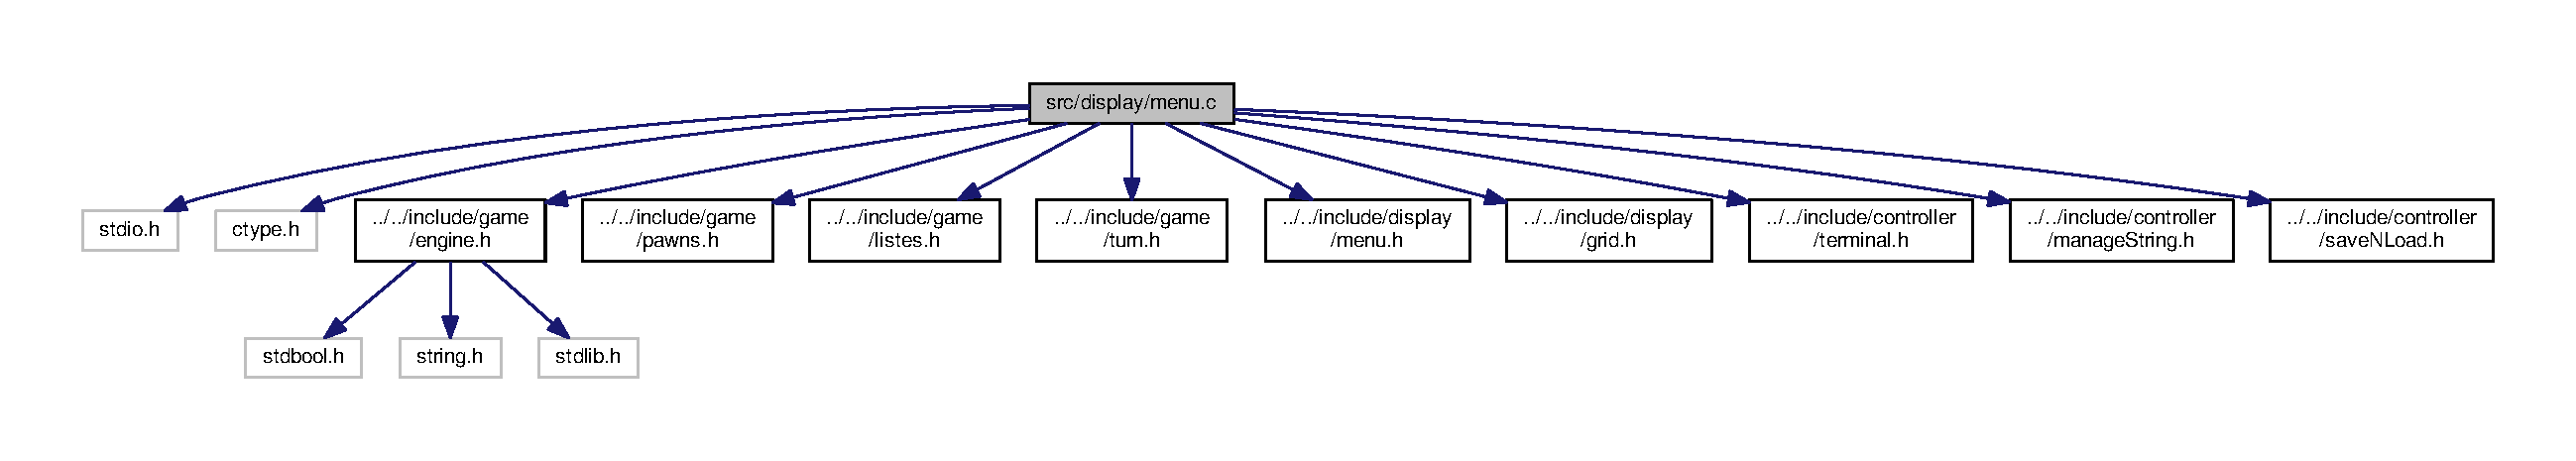
\includegraphics[width=350pt]{menu_8c__incl}
\end{center}
\end{figure}
\subsection*{Fonctions}
\begin{DoxyCompactItemize}
\item 
void \hyperlink{menu_8c_ab3002fe8e0074c9e2ecb5b835e5e819f}{main\+Menu} ()
\begin{DoxyCompactList}\small\item\em Menu principal du jeu. \end{DoxyCompactList}\item 
\hypertarget{menu_8c_a57c1286e99f7c479a937ebbafcfe8681}{}void \hyperlink{menu_8c_a57c1286e99f7c479a937ebbafcfe8681}{main\+Help} ()\label{menu_8c_a57c1286e99f7c479a937ebbafcfe8681}

\begin{DoxyCompactList}\small\item\em Menu d\textquotesingle{}aide principal. \end{DoxyCompactList}\item 
void \hyperlink{menu_8c_aea4bcea967e5f0d7bb00517649f21701}{help\+Unit} ()
\begin{DoxyCompactList}\small\item\em Menu d\textquotesingle{}aide spéifique aux unités. \end{DoxyCompactList}\item 
void \hyperlink{menu_8c_aac6cc2265bfc1481caf987f92bece27b}{disp\+Direction} ()
\begin{DoxyCompactList}\small\item\em Afficher les directions. \end{DoxyCompactList}\item 
void \hyperlink{menu_8c_ac722505df6f214afc5d28c922da5e0c7}{game\+Menu} ()
\begin{DoxyCompactList}\small\item\em Menu du joueur lors de la partie. \end{DoxyCompactList}\item 
void \hyperlink{menu_8c_a4e88525c8d42c1affc4e8ef8e7ebca44}{unit\+Menu} (int choice)
\begin{DoxyCompactList}\small\item\em Menu de sélection de l\textquotesingle{}unité \end{DoxyCompactList}\item 
void \hyperlink{menu_8c_a2eb7eed865e161dfaf02136f6c22e873}{unit\+List} ()
\begin{DoxyCompactList}\small\item\em Affiche la liste des unités inclus dans le jeu. \end{DoxyCompactList}\end{DoxyCompactItemize}


\subsection{Description détaillée}
Gestion des menus. 

\begin{DoxyAuthor}{Auteur}
Cousin Brandon Chaudemanche Ewen Biardeau Tristan 
\end{DoxyAuthor}
\begin{DoxyVersion}{Version}
v1.\+00 
\end{DoxyVersion}
\begin{DoxyDate}{Date}
18/12/2015 
\end{DoxyDate}


\subsection{Documentation des fonctions}
\hypertarget{menu_8c_aac6cc2265bfc1481caf987f92bece27b}{}\index{menu.\+c@{menu.\+c}!disp\+Direction@{disp\+Direction}}
\index{disp\+Direction@{disp\+Direction}!menu.\+c@{menu.\+c}}
\subsubsection[{disp\+Direction}]{\setlength{\rightskip}{0pt plus 5cm}void disp\+Direction (
\begin{DoxyParamCaption}
{}
\end{DoxyParamCaption}
)}\label{menu_8c_aac6cc2265bfc1481caf987f92bece27b}


Afficher les directions. 

Affiche la liste des directions. 

Définition à la ligne 458 du fichier menu.\+c.

\hypertarget{menu_8c_ac722505df6f214afc5d28c922da5e0c7}{}\index{menu.\+c@{menu.\+c}!game\+Menu@{game\+Menu}}
\index{game\+Menu@{game\+Menu}!menu.\+c@{menu.\+c}}
\subsubsection[{game\+Menu}]{\setlength{\rightskip}{0pt plus 5cm}void game\+Menu (
\begin{DoxyParamCaption}
{}
\end{DoxyParamCaption}
)}\label{menu_8c_ac722505df6f214afc5d28c922da5e0c7}


Menu du joueur lors de la partie. 

Menu de jeu. 

Définition à la ligne 470 du fichier menu.\+c.

\hypertarget{menu_8c_aea4bcea967e5f0d7bb00517649f21701}{}\index{menu.\+c@{menu.\+c}!help\+Unit@{help\+Unit}}
\index{help\+Unit@{help\+Unit}!menu.\+c@{menu.\+c}}
\subsubsection[{help\+Unit}]{\setlength{\rightskip}{0pt plus 5cm}void help\+Unit (
\begin{DoxyParamCaption}
{}
\end{DoxyParamCaption}
)}\label{menu_8c_aea4bcea967e5f0d7bb00517649f21701}


Menu d\textquotesingle{}aide spéifique aux unités. 

Menu d\textquotesingle{}aide des unités. 

Définition à la ligne 222 du fichier menu.\+c.

\hypertarget{menu_8c_ab3002fe8e0074c9e2ecb5b835e5e819f}{}\index{menu.\+c@{menu.\+c}!main\+Menu@{main\+Menu}}
\index{main\+Menu@{main\+Menu}!menu.\+c@{menu.\+c}}
\subsubsection[{main\+Menu}]{\setlength{\rightskip}{0pt plus 5cm}void main\+Menu (
\begin{DoxyParamCaption}
{}
\end{DoxyParamCaption}
)}\label{menu_8c_ab3002fe8e0074c9e2ecb5b835e5e819f}


Menu principal du jeu. 

Menu principal. 

Définition à la ligne 24 du fichier menu.\+c.

\hypertarget{menu_8c_a2eb7eed865e161dfaf02136f6c22e873}{}\index{menu.\+c@{menu.\+c}!unit\+List@{unit\+List}}
\index{unit\+List@{unit\+List}!menu.\+c@{menu.\+c}}
\subsubsection[{unit\+List}]{\setlength{\rightskip}{0pt plus 5cm}void unit\+List (
\begin{DoxyParamCaption}
{}
\end{DoxyParamCaption}
)}\label{menu_8c_a2eb7eed865e161dfaf02136f6c22e873}


Affiche la liste des unités inclus dans le jeu. 

Listes des unités du jeu. 

Définition à la ligne 593 du fichier menu.\+c.

\hypertarget{menu_8c_a4e88525c8d42c1affc4e8ef8e7ebca44}{}\index{menu.\+c@{menu.\+c}!unit\+Menu@{unit\+Menu}}
\index{unit\+Menu@{unit\+Menu}!menu.\+c@{menu.\+c}}
\subsubsection[{unit\+Menu}]{\setlength{\rightskip}{0pt plus 5cm}void unit\+Menu (
\begin{DoxyParamCaption}
\item[{int}]{choice}
\end{DoxyParamCaption}
)}\label{menu_8c_a4e88525c8d42c1affc4e8ef8e7ebca44}


Menu de sélection de l\textquotesingle{}unité 


\begin{DoxyParams}{Paramètres}
{\em choice} & Choix de l\textquotesingle{}action pour l\textquotesingle{}unité \\
\hline
\end{DoxyParams}


Définition à la ligne 517 du fichier menu.\+c.


\hypertarget{engine_8c}{}\section{Référence du fichier src/game/engine.c}
\label{engine_8c}\index{src/game/engine.\+c@{src/game/engine.\+c}}


Moteur de jeu.  


{\ttfamily \#include $<$stdio.\+h$>$}\\*
{\ttfamily \#include $<$time.\+h$>$}\\*
{\ttfamily \#include \char`\"{}../../include/game/engine.\+h\char`\"{}}\\*
{\ttfamily \#include \char`\"{}../../include/game/pawns.\+h\char`\"{}}\\*
{\ttfamily \#include \char`\"{}../../include/game/path\+List.\+h\char`\"{}}\\*
{\ttfamily \#include \char`\"{}../../include/game/listes.\+h\char`\"{}}\\*
{\ttfamily \#include \char`\"{}../../include/game/turn.\+h\char`\"{}}\\*
{\ttfamily \#include \char`\"{}../../include/display/grid.\+h\char`\"{}}\\*
{\ttfamily \#include \char`\"{}../../include/display/menu.\+h\char`\"{}}\\*
{\ttfamily \#include \char`\"{}../../include/controller/terminal.\+h\char`\"{}}\\*
{\ttfamily \#include \char`\"{}../../include/controller/manage\+String.\+h\char`\"{}}\\*
{\ttfamily \#include \char`\"{}../../include/controller/manage\+Signal.\+h\char`\"{}}\\*
{\ttfamily \#include \char`\"{}../../include/units/unit.\+h\char`\"{}}\\*
Graphe des dépendances par inclusion de engine.\+c\+:\nopagebreak
\begin{figure}[H]
\begin{center}
\leavevmode
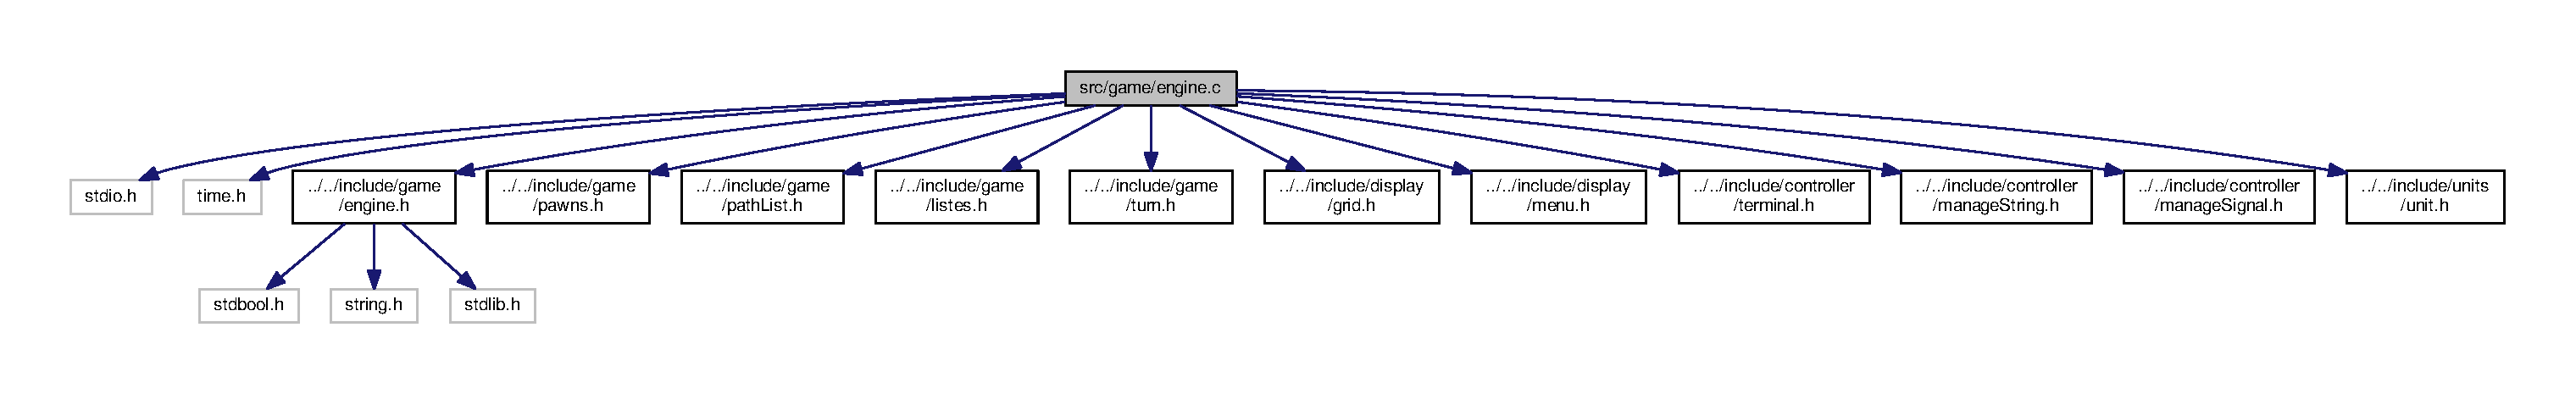
\includegraphics[width=350pt]{engine_8c__incl}
\end{center}
\end{figure}
\subsection*{Fonctions}
\begin{DoxyCompactItemize}
\item 
bool \hyperlink{engine_8c_a548c013433afab60c17fd9950fb7248f}{possible\+Path} (\hyperlink{structvector}{vector} coord\+Unit)
\begin{DoxyCompactList}\small\item\em Trouve un chemin vers une quelconque position pour l\textquotesingle{}unité \end{DoxyCompactList}\item 
bool \hyperlink{engine_8c_a2790b2bcc6484aa19c0319ed791c9993}{path\+Find} (\hyperlink{structvector}{vector} coord\+Unit, \hyperlink{structvector}{vector} coord\+Target)
\begin{DoxyCompactList}\small\item\em Trouve un chemin vers la position désirée. \end{DoxyCompactList}\item 
void \hyperlink{engine_8c_a8e572eb4d2e9c66a18ead32ae6f37152}{line\+Of\+Sight} (\hyperlink{structvector}{vector} coord\+Source, \hyperlink{structvector}{vector} coord\+Target)
\begin{DoxyCompactList}\small\item\em Ligne de vue de l\textquotesingle{}archer. \end{DoxyCompactList}\item 
void \hyperlink{engine_8c_a8aca0579aac39cc7e3c41342d89fe1b7}{movable} (int color\+Disp)
\begin{DoxyCompactList}\small\item\em Fait la liste des unités déplaçables. \end{DoxyCompactList}\item 
void \hyperlink{engine_8c_ae40e16d551936cea056a982196273bde}{attackable} (int color\+Disp)
\begin{DoxyCompactList}\small\item\em Fait la liste des unités pouvant attaquer. \end{DoxyCompactList}\item 
void \hyperlink{engine_8c_a309311c2d6a59c5998007d0e5f215d4d}{tile\+Walkable} (\hyperlink{structvector}{vector} coord\+Unit, int color\+Disp)
\begin{DoxyCompactList}\small\item\em Fait la liste des cases pouvant être atteintes par l\textquotesingle{}unité \end{DoxyCompactList}\item 
bool \hyperlink{engine_8c_a3ee2a4066924757ade5530e7041a2ad1}{is\+Surrounded} (\hyperlink{structvector}{vector} current\+Unit)
\begin{DoxyCompactList}\small\item\em Permet de savoir si l\textquotesingle{}unité courante est entourée. \end{DoxyCompactList}\item 
void \hyperlink{engine_8c_a7de2811c781a1136844609cc95e26464}{set\+Target} (\hyperlink{engine_8h_af7667555c2dcfbdd55ec3e9dd6a907ba}{unit\+Name} name, \hyperlink{structvector}{vector} coord\+Unit, int color\+Disp)
\begin{DoxyCompactList}\small\item\em Initialise les cibles du pion. \end{DoxyCompactList}\item 
void \hyperlink{engine_8c_af7fe21fb0c7ba2b2823eac899e12a5cd}{special\+Boons} (\hyperlink{structvector}{vector} coord\+Source, \hyperlink{structvector}{vector} coord\+Target)
\begin{DoxyCompactList}\small\item\em Déclenche une capacité spéciale selon l\textquotesingle{}unité \end{DoxyCompactList}\item 
void \hyperlink{engine_8c_a42359e6294ac21935ecc2d77140da492}{launch\+Attack} (\hyperlink{structvector}{vector} coord\+Source, \hyperlink{structvector}{vector} coord\+Target)
\begin{DoxyCompactList}\small\item\em Lance une attaque selon l\textquotesingle{}unité \end{DoxyCompactList}\item 
bool \hyperlink{engine_8c_acd459b9ed1aaf8c05cdd3887e86b8668}{select\+Unit} (\hyperlink{structvector}{vector} $\ast$coord\+Unit)
\begin{DoxyCompactList}\small\item\em Sélectionne une unité \end{DoxyCompactList}\item 
\hypertarget{engine_8c_aeaf554c67cf57c6e627d29731c7d7ae3}{}void \hyperlink{engine_8c_aeaf554c67cf57c6e627d29731c7d7ae3}{grid\+Init} ()\label{engine_8c_aeaf554c67cf57c6e627d29731c7d7ae3}

\begin{DoxyCompactList}\small\item\em Initialise la grille. \end{DoxyCompactList}\item 
bool \hyperlink{engine_8c_a618bf94529881cb216645f79ff8d2f83}{too\+Much\+Unit} (int unit\+Selected, int limit\+Units\mbox{[}$\,$\mbox{]})
\begin{DoxyCompactList}\small\item\em Vérifie que l\textquotesingle{}unité sélectionnée n\textquotesingle{}est pas en trop grand nombre sur le plateau. \end{DoxyCompactList}\item 
void \hyperlink{engine_8c_aa97fb26c7cc91c4937b281c4c1be9230}{update\+Limits} (int unit\+Selected, int limit\+Units\mbox{[}$\,$\mbox{]}, \hyperlink{structvector}{vector} coord\+Unit)
\begin{DoxyCompactList}\small\item\em Met à jour les limites d\textquotesingle{}unités. \end{DoxyCompactList}\item 
void \hyperlink{engine_8c_a9179a9a94e1bdad5a01584f45133f992}{ask\+Unit} (int $\ast$unit\+Selected, int limit\+Units\mbox{[}$\,$\mbox{]})
\begin{DoxyCompactList}\small\item\em Demande de choisir une unité \end{DoxyCompactList}\item 
void \hyperlink{engine_8c_a267dcffc14ba303f11040bec890cb864}{ask\+Coord} (char coord\+String\mbox{[}$\,$\mbox{]})
\begin{DoxyCompactList}\small\item\em Demande les coordonnées de l\textquotesingle{}unité à placer. \end{DoxyCompactList}\item 
void \hyperlink{engine_8c_a3b85862a0c5139738dae78042d1e9977}{player\+Add\+Unit} (int limit\+Units\mbox{[}$\,$\mbox{]}, int $\ast$nb\+Unit)
\begin{DoxyCompactList}\small\item\em Placement des unités par le joueur. \end{DoxyCompactList}\item 
\hypertarget{engine_8c_ad8a24588946876bf7ba9aa7217091387}{}void \hyperlink{engine_8c_ad8a24588946876bf7ba9aa7217091387}{player\+Init} ()\label{engine_8c_ad8a24588946876bf7ba9aa7217091387}

\begin{DoxyCompactList}\small\item\em Initiliase la liste des unités du joueur. \end{DoxyCompactList}\item 
\hypertarget{engine_8c_a7ece650b518ffb4d0312b822cdf31517}{}bool \hyperlink{engine_8c_a7ece650b518ffb4d0312b822cdf31517}{end\+Game} ()\label{engine_8c_a7ece650b518ffb4d0312b822cdf31517}

\begin{DoxyCompactList}\small\item\em Fin de la partie. \end{DoxyCompactList}\item 
\hypertarget{engine_8c_ab1f321a2f17fa8ba0f5ab4e2621fd6d6}{}void \hyperlink{engine_8c_ab1f321a2f17fa8ba0f5ab4e2621fd6d6}{start\+Game} ()\label{engine_8c_ab1f321a2f17fa8ba0f5ab4e2621fd6d6}

\begin{DoxyCompactList}\small\item\em Débute la partie. \end{DoxyCompactList}\item 
void \hyperlink{engine_8c_a43ae9a7f0ac55585ed6375c580abcaf0}{game\+Init} ()
\begin{DoxyCompactList}\small\item\em Initialise la partie. \end{DoxyCompactList}\end{DoxyCompactItemize}
\subsection*{Variables}
\begin{DoxyCompactItemize}
\item 
\hyperlink{structunit}{unit} \hyperlink{engine_8c_a5987e3369c71f1edb157786e4c75875b}{grid} \mbox{[}\hyperlink{engine_8h_a0240ac851181b84ac374872dc5434ee4}{N}\mbox{]}\mbox{[}\hyperlink{engine_8h_a0240ac851181b84ac374872dc5434ee4}{N}\mbox{]}
\begin{DoxyCompactList}\small\item\em Grille d\textquotesingle{}unités. \end{DoxyCompactList}\item 
int \hyperlink{engine_8c_afaa2c64a9fd09c382394b57006c470ce}{no\+Player} = \hyperlink{engine_8h_a89f0201fca94cbc3ca0f5fbce851e7c9}{F\+I\+R\+S\+T\+\_\+\+P\+L\+A\+Y\+E\+R}
\begin{DoxyCompactList}\small\item\em Joueur en cours. \end{DoxyCompactList}\end{DoxyCompactItemize}


\subsection{Description détaillée}
Moteur de jeu. 

\begin{DoxyAuthor}{Auteur}
Cousin Brandon Chaudemanche Ewen Biardeau Tristan 
\end{DoxyAuthor}
\begin{DoxyVersion}{Version}
v1.\+00 
\end{DoxyVersion}
\begin{DoxyDate}{Date}
18/12/2015 
\end{DoxyDate}


\subsection{Documentation des fonctions}
\hypertarget{engine_8c_a267dcffc14ba303f11040bec890cb864}{}\index{engine.\+c@{engine.\+c}!ask\+Coord@{ask\+Coord}}
\index{ask\+Coord@{ask\+Coord}!engine.\+c@{engine.\+c}}
\subsubsection[{ask\+Coord}]{\setlength{\rightskip}{0pt plus 5cm}void ask\+Coord (
\begin{DoxyParamCaption}
\item[{char}]{coord\+String\mbox{[}$\,$\mbox{]}}
\end{DoxyParamCaption}
)}\label{engine_8c_a267dcffc14ba303f11040bec890cb864}


Demande les coordonnées de l\textquotesingle{}unité à placer. 


\begin{DoxyParams}{Paramètres}
{\em coord\+String} & Coordonnées sous forme de chaîne \\
\hline
\end{DoxyParams}


Définition à la ligne 579 du fichier engine.\+c.

\hypertarget{engine_8c_a9179a9a94e1bdad5a01584f45133f992}{}\index{engine.\+c@{engine.\+c}!ask\+Unit@{ask\+Unit}}
\index{ask\+Unit@{ask\+Unit}!engine.\+c@{engine.\+c}}
\subsubsection[{ask\+Unit}]{\setlength{\rightskip}{0pt plus 5cm}void ask\+Unit (
\begin{DoxyParamCaption}
\item[{int $\ast$}]{unit\+Selected, }
\item[{int}]{limit\+Units\mbox{[}$\,$\mbox{]}}
\end{DoxyParamCaption}
)}\label{engine_8c_a9179a9a94e1bdad5a01584f45133f992}


Demande de choisir une unité 


\begin{DoxyParams}{Paramètres}
{\em unit\+Selected} & Unité sélectionnée \\
\hline
{\em limit\+Units} & Nombre limite pour chaque unité \\
\hline
\end{DoxyParams}


Définition à la ligne 551 du fichier engine.\+c.

\hypertarget{engine_8c_ae40e16d551936cea056a982196273bde}{}\index{engine.\+c@{engine.\+c}!attackable@{attackable}}
\index{attackable@{attackable}!engine.\+c@{engine.\+c}}
\subsubsection[{attackable}]{\setlength{\rightskip}{0pt plus 5cm}void attackable (
\begin{DoxyParamCaption}
\item[{int}]{color\+Disp}
\end{DoxyParamCaption}
)}\label{engine_8c_ae40e16d551936cea056a982196273bde}


Fait la liste des unités pouvant attaquer. 


\begin{DoxyParams}{Paramètres}
{\em color\+Disp} & Couleur d\textquotesingle{}affichage \\
\hline
\end{DoxyParams}


Définition à la ligne 164 du fichier engine.\+c.

\hypertarget{engine_8c_a43ae9a7f0ac55585ed6375c580abcaf0}{}\index{engine.\+c@{engine.\+c}!game\+Init@{game\+Init}}
\index{game\+Init@{game\+Init}!engine.\+c@{engine.\+c}}
\subsubsection[{game\+Init}]{\setlength{\rightskip}{0pt plus 5cm}void game\+Init (
\begin{DoxyParamCaption}
{}
\end{DoxyParamCaption}
)}\label{engine_8c_a43ae9a7f0ac55585ed6375c580abcaf0}


Initialise la partie. 

Initialise le jeu. 

Définition à la ligne 750 du fichier engine.\+c.

\hypertarget{engine_8c_a3ee2a4066924757ade5530e7041a2ad1}{}\index{engine.\+c@{engine.\+c}!is\+Surrounded@{is\+Surrounded}}
\index{is\+Surrounded@{is\+Surrounded}!engine.\+c@{engine.\+c}}
\subsubsection[{is\+Surrounded}]{\setlength{\rightskip}{0pt plus 5cm}bool is\+Surrounded (
\begin{DoxyParamCaption}
\item[{{\bf vector}}]{current\+Unit}
\end{DoxyParamCaption}
)}\label{engine_8c_a3ee2a4066924757ade5530e7041a2ad1}


Permet de savoir si l\textquotesingle{}unité courante est entourée. 

Vérifie si une unité est entourée.


\begin{DoxyParams}{Paramètres}
{\em current\+Unit} & Unité courante \\
\hline
\end{DoxyParams}
\begin{DoxyReturn}{Renvoie}
Retourne vrai si unité entourée 
\end{DoxyReturn}


Définition à la ligne 215 du fichier engine.\+c.

\hypertarget{engine_8c_a42359e6294ac21935ecc2d77140da492}{}\index{engine.\+c@{engine.\+c}!launch\+Attack@{launch\+Attack}}
\index{launch\+Attack@{launch\+Attack}!engine.\+c@{engine.\+c}}
\subsubsection[{launch\+Attack}]{\setlength{\rightskip}{0pt plus 5cm}void launch\+Attack (
\begin{DoxyParamCaption}
\item[{{\bf vector}}]{coord\+Source, }
\item[{{\bf vector}}]{coord\+Target}
\end{DoxyParamCaption}
)}\label{engine_8c_a42359e6294ac21935ecc2d77140da492}


Lance une attaque selon l\textquotesingle{}unité 

Lance une attaque.


\begin{DoxyParams}{Paramètres}
{\em coord\+Source} & Nom de l\textquotesingle{}unité source \\
\hline
{\em coord\+Target} & Coordonnées de la cible \\
\hline
\end{DoxyParams}


Définition à la ligne 336 du fichier engine.\+c.

\hypertarget{engine_8c_a8e572eb4d2e9c66a18ead32ae6f37152}{}\index{engine.\+c@{engine.\+c}!line\+Of\+Sight@{line\+Of\+Sight}}
\index{line\+Of\+Sight@{line\+Of\+Sight}!engine.\+c@{engine.\+c}}
\subsubsection[{line\+Of\+Sight}]{\setlength{\rightskip}{0pt plus 5cm}void line\+Of\+Sight (
\begin{DoxyParamCaption}
\item[{{\bf vector}}]{coord\+Source, }
\item[{{\bf vector}}]{coord\+Target}
\end{DoxyParamCaption}
)}\label{engine_8c_a8e572eb4d2e9c66a18ead32ae6f37152}


Ligne de vue de l\textquotesingle{}archer. 


\begin{DoxyParams}{Paramètres}
{\em coord\+Source} & Coordonnées de l\textquotesingle{}unité attaquante \\
\hline
{\em coord\+Target} & Coordonnées de la cible \\
\hline
\end{DoxyParams}


Définition à la ligne 117 du fichier engine.\+c.

\hypertarget{engine_8c_a8aca0579aac39cc7e3c41342d89fe1b7}{}\index{engine.\+c@{engine.\+c}!movable@{movable}}
\index{movable@{movable}!engine.\+c@{engine.\+c}}
\subsubsection[{movable}]{\setlength{\rightskip}{0pt plus 5cm}void movable (
\begin{DoxyParamCaption}
\item[{int}]{color\+Disp}
\end{DoxyParamCaption}
)}\label{engine_8c_a8aca0579aac39cc7e3c41342d89fe1b7}


Fait la liste des unités déplaçables. 


\begin{DoxyParams}{Paramètres}
{\em color\+Disp} & Couleur d\textquotesingle{}affichage \\
\hline
\end{DoxyParams}


Définition à la ligne 141 du fichier engine.\+c.

\hypertarget{engine_8c_a2790b2bcc6484aa19c0319ed791c9993}{}\index{engine.\+c@{engine.\+c}!path\+Find@{path\+Find}}
\index{path\+Find@{path\+Find}!engine.\+c@{engine.\+c}}
\subsubsection[{path\+Find}]{\setlength{\rightskip}{0pt plus 5cm}bool path\+Find (
\begin{DoxyParamCaption}
\item[{{\bf vector}}]{coord\+Unit, }
\item[{{\bf vector}}]{coord\+Target}
\end{DoxyParamCaption}
)}\label{engine_8c_a2790b2bcc6484aa19c0319ed791c9993}


Trouve un chemin vers la position désirée. 

Trouve une chemin vers la destination.


\begin{DoxyParams}{Paramètres}
{\em coord\+Unit} & Coordonnées de l\textquotesingle{}unité \\
\hline
{\em coord\+Target} & Coordonnées de la cible \\
\hline
\end{DoxyParams}
\begin{DoxyReturn}{Renvoie}
Retourne vrai si chemin trouvé 
\end{DoxyReturn}


Définition à la ligne 60 du fichier engine.\+c.

\hypertarget{engine_8c_a3b85862a0c5139738dae78042d1e9977}{}\index{engine.\+c@{engine.\+c}!player\+Add\+Unit@{player\+Add\+Unit}}
\index{player\+Add\+Unit@{player\+Add\+Unit}!engine.\+c@{engine.\+c}}
\subsubsection[{player\+Add\+Unit}]{\setlength{\rightskip}{0pt plus 5cm}void player\+Add\+Unit (
\begin{DoxyParamCaption}
\item[{int}]{limit\+Units\mbox{[}$\,$\mbox{]}, }
\item[{int $\ast$}]{nb\+Unit}
\end{DoxyParamCaption}
)}\label{engine_8c_a3b85862a0c5139738dae78042d1e9977}


Placement des unités par le joueur. 


\begin{DoxyParams}{Paramètres}
{\em limit\+Units} & Limites d\textquotesingle{}unités \\
\hline
{\em nb\+Unit} & Nombre d\textquotesingle{}unités restantes à placer \\
\hline
\end{DoxyParams}


Définition à la ligne 608 du fichier engine.\+c.

\hypertarget{engine_8c_a548c013433afab60c17fd9950fb7248f}{}\index{engine.\+c@{engine.\+c}!possible\+Path@{possible\+Path}}
\index{possible\+Path@{possible\+Path}!engine.\+c@{engine.\+c}}
\subsubsection[{possible\+Path}]{\setlength{\rightskip}{0pt plus 5cm}bool possible\+Path (
\begin{DoxyParamCaption}
\item[{{\bf vector}}]{coord\+Unit}
\end{DoxyParamCaption}
)}\label{engine_8c_a548c013433afab60c17fd9950fb7248f}


Trouve un chemin vers une quelconque position pour l\textquotesingle{}unité 

Vérifie qu\textquotesingle{}un chemin est possible.


\begin{DoxyParams}{Paramètres}
{\em coord\+Unit} & Coordonnées de l\textquotesingle{}unité \\
\hline
\end{DoxyParams}
\begin{DoxyReturn}{Renvoie}
Retourne Vrai si chemin possible vers une quelconque position 
\end{DoxyReturn}


Définition à la ligne 31 du fichier engine.\+c.

\hypertarget{engine_8c_acd459b9ed1aaf8c05cdd3887e86b8668}{}\index{engine.\+c@{engine.\+c}!select\+Unit@{select\+Unit}}
\index{select\+Unit@{select\+Unit}!engine.\+c@{engine.\+c}}
\subsubsection[{select\+Unit}]{\setlength{\rightskip}{0pt plus 5cm}bool select\+Unit (
\begin{DoxyParamCaption}
\item[{{\bf vector} $\ast$}]{coord\+Unit}
\end{DoxyParamCaption}
)}\label{engine_8c_acd459b9ed1aaf8c05cdd3887e86b8668}


Sélectionne une unité 


\begin{DoxyParams}{Paramètres}
{\em coord\+Unit} & Coordoonnées de l\textquotesingle{}unité \\
\hline
\end{DoxyParams}
\begin{DoxyReturn}{Renvoie}
Retourne vrai si unité bien sélectionnée 
\end{DoxyReturn}


Définition à la ligne 416 du fichier engine.\+c.

\hypertarget{engine_8c_a7de2811c781a1136844609cc95e26464}{}\index{engine.\+c@{engine.\+c}!set\+Target@{set\+Target}}
\index{set\+Target@{set\+Target}!engine.\+c@{engine.\+c}}
\subsubsection[{set\+Target}]{\setlength{\rightskip}{0pt plus 5cm}void set\+Target (
\begin{DoxyParamCaption}
\item[{{\bf unit\+Name}}]{name, }
\item[{{\bf vector}}]{coord\+Unit, }
\item[{int}]{color\+Disp}
\end{DoxyParamCaption}
)}\label{engine_8c_a7de2811c781a1136844609cc95e26464}


Initialise les cibles du pion. 

Définis les cibles.


\begin{DoxyParams}{Paramètres}
{\em name} & Nom du pion \\
\hline
{\em coord\+Unit} & Coordonnées de l\textquotesingle{}unité \\
\hline
{\em color\+Disp} & Couleur d\textquotesingle{}affichage \\
\hline
\end{DoxyParams}


Définition à la ligne 252 du fichier engine.\+c.

\hypertarget{engine_8c_af7fe21fb0c7ba2b2823eac899e12a5cd}{}\index{engine.\+c@{engine.\+c}!special\+Boons@{special\+Boons}}
\index{special\+Boons@{special\+Boons}!engine.\+c@{engine.\+c}}
\subsubsection[{special\+Boons}]{\setlength{\rightskip}{0pt plus 5cm}void special\+Boons (
\begin{DoxyParamCaption}
\item[{{\bf vector}}]{coord\+Source, }
\item[{{\bf vector}}]{coord\+Target}
\end{DoxyParamCaption}
)}\label{engine_8c_af7fe21fb0c7ba2b2823eac899e12a5cd}


Déclenche une capacité spéciale selon l\textquotesingle{}unité 


\begin{DoxyParams}{Paramètres}
{\em coord\+Source} & Coordonnées de l\textquotesingle{}unité source (déclenchant une capacité) \\
\hline
{\em coord\+Target} & Coordonnées de l\textquotesingle{}unité affectée par la capacité spéciale \\
\hline
\end{DoxyParams}


Définition à la ligne 299 du fichier engine.\+c.

\hypertarget{engine_8c_a309311c2d6a59c5998007d0e5f215d4d}{}\index{engine.\+c@{engine.\+c}!tile\+Walkable@{tile\+Walkable}}
\index{tile\+Walkable@{tile\+Walkable}!engine.\+c@{engine.\+c}}
\subsubsection[{tile\+Walkable}]{\setlength{\rightskip}{0pt plus 5cm}void tile\+Walkable (
\begin{DoxyParamCaption}
\item[{{\bf vector}}]{coord\+Unit, }
\item[{int}]{color\+Disp}
\end{DoxyParamCaption}
)}\label{engine_8c_a309311c2d6a59c5998007d0e5f215d4d}


Fait la liste des cases pouvant être atteintes par l\textquotesingle{}unité 

Fait la liste des cases atteignables par l\textquotesingle{}unité


\begin{DoxyParams}{Paramètres}
{\em coord\+Unit} & Coordonnées de l\textquotesingle{}unité \\
\hline
{\em color\+Disp} & Couleur d\textquotesingle{}affichage \\
\hline
\end{DoxyParams}


Définition à la ligne 188 du fichier engine.\+c.

\hypertarget{engine_8c_a618bf94529881cb216645f79ff8d2f83}{}\index{engine.\+c@{engine.\+c}!too\+Much\+Unit@{too\+Much\+Unit}}
\index{too\+Much\+Unit@{too\+Much\+Unit}!engine.\+c@{engine.\+c}}
\subsubsection[{too\+Much\+Unit}]{\setlength{\rightskip}{0pt plus 5cm}bool too\+Much\+Unit (
\begin{DoxyParamCaption}
\item[{int}]{unit\+Selected, }
\item[{int}]{limit\+Units\mbox{[}$\,$\mbox{]}}
\end{DoxyParamCaption}
)}\label{engine_8c_a618bf94529881cb216645f79ff8d2f83}


Vérifie que l\textquotesingle{}unité sélectionnée n\textquotesingle{}est pas en trop grand nombre sur le plateau. 


\begin{DoxyParams}{Paramètres}
{\em unit\+Selected} & Unité sélectionnée \\
\hline
{\em limit\+Units} & Tableau des limites pour chaque unité \\
\hline
\end{DoxyParams}
\begin{DoxyReturn}{Renvoie}
Retourne vrai si unité en surnombre 
\end{DoxyReturn}


Définition à la ligne 468 du fichier engine.\+c.

\hypertarget{engine_8c_aa97fb26c7cc91c4937b281c4c1be9230}{}\index{engine.\+c@{engine.\+c}!update\+Limits@{update\+Limits}}
\index{update\+Limits@{update\+Limits}!engine.\+c@{engine.\+c}}
\subsubsection[{update\+Limits}]{\setlength{\rightskip}{0pt plus 5cm}void update\+Limits (
\begin{DoxyParamCaption}
\item[{int}]{unit\+Selected, }
\item[{int}]{limit\+Units\mbox{[}$\,$\mbox{]}, }
\item[{{\bf vector}}]{coord\+Unit}
\end{DoxyParamCaption}
)}\label{engine_8c_aa97fb26c7cc91c4937b281c4c1be9230}


Met à jour les limites d\textquotesingle{}unités. 


\begin{DoxyParams}{Paramètres}
{\em unit\+Selected} & Unité sélectionnée \\
\hline
{\em limit\+Units} & Limites liées aux unités sur le plateau \\
\hline
{\em coord\+Unit} & Coordonnées de l\textquotesingle{}unité \\
\hline
\end{DoxyParams}


Définition à la ligne 515 du fichier engine.\+c.



\subsection{Documentation des variables}
\hypertarget{engine_8c_a5987e3369c71f1edb157786e4c75875b}{}\index{engine.\+c@{engine.\+c}!grid@{grid}}
\index{grid@{grid}!engine.\+c@{engine.\+c}}
\subsubsection[{grid}]{\setlength{\rightskip}{0pt plus 5cm}{\bf unit} grid\mbox{[}{\bf N}\mbox{]}\mbox{[}{\bf N}\mbox{]}}\label{engine_8c_a5987e3369c71f1edb157786e4c75875b}


Grille d\textquotesingle{}unités. 

Représentation d\textquotesingle{}une grille d\textquotesingle{}unité globale. 

Définition à la ligne 23 du fichier engine.\+c.

\hypertarget{engine_8c_afaa2c64a9fd09c382394b57006c470ce}{}\index{engine.\+c@{engine.\+c}!no\+Player@{no\+Player}}
\index{no\+Player@{no\+Player}!engine.\+c@{engine.\+c}}
\subsubsection[{no\+Player}]{\setlength{\rightskip}{0pt plus 5cm}int no\+Player = {\bf F\+I\+R\+S\+T\+\_\+\+P\+L\+A\+Y\+E\+R}}\label{engine_8c_afaa2c64a9fd09c382394b57006c470ce}


Joueur en cours. 

Représentation du joueur. 

Définition à la ligne 24 du fichier engine.\+c.


\hypertarget{listes_8c}{}\section{Référence du fichier src/game/listes.c}
\label{listes_8c}\index{src/game/listes.\+c@{src/game/listes.\+c}}


Listes de vecteurs.  


{\ttfamily \#include $<$stdio.\+h$>$}\\*
{\ttfamily \#include \char`\"{}../../include/game/engine.\+h\char`\"{}}\\*
{\ttfamily \#include \char`\"{}../../include/game/pawns.\+h\char`\"{}}\\*
{\ttfamily \#include \char`\"{}../../include/controller/manage\+String.\+h\char`\"{}}\\*
{\ttfamily \#include \char`\"{}../../include/game/listes.\+h\char`\"{}}\\*
Graphe des dépendances par inclusion de listes.\+c\+:\nopagebreak
\begin{figure}[H]
\begin{center}
\leavevmode
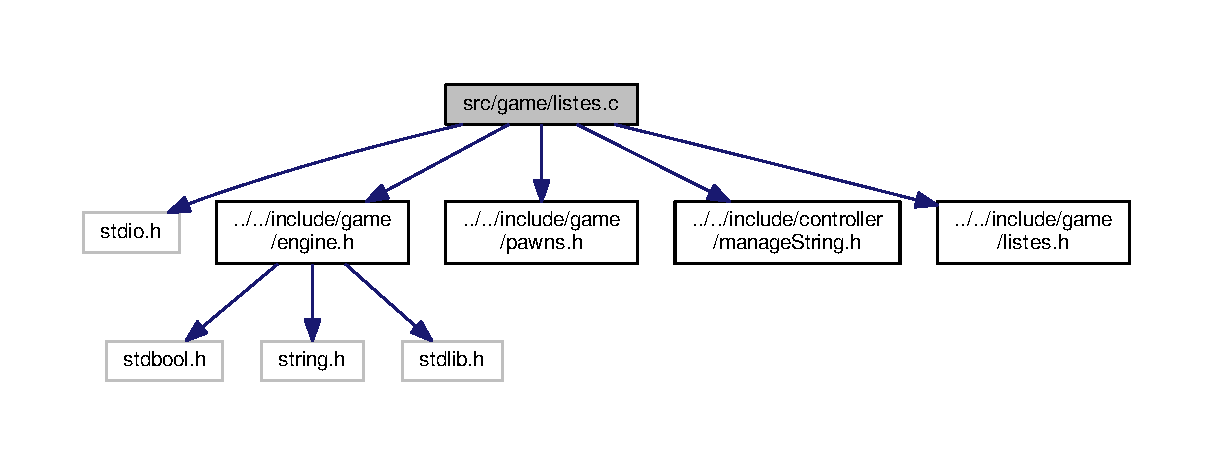
\includegraphics[width=350pt]{listes_8c__incl}
\end{center}
\end{figure}
\subsection*{Classes}
\begin{DoxyCompactItemize}
\item 
struct \hyperlink{structelement}{element}
\begin{DoxyCompactList}\small\item\em Représente un élément de la liste. \end{DoxyCompactList}\end{DoxyCompactItemize}
\subsection*{Définitions de type}
\begin{DoxyCompactItemize}
\item 
\hypertarget{listes_8c_a8968705d25c62eaf27310fae6cc2603f}{}typedef struct \hyperlink{structelement}{element} \hyperlink{listes_8c_a8968705d25c62eaf27310fae6cc2603f}{t\+\_\+element}\label{listes_8c_a8968705d25c62eaf27310fae6cc2603f}

\begin{DoxyCompactList}\small\item\em Définis un élément. \end{DoxyCompactList}\end{DoxyCompactItemize}
\subsection*{Fonctions}
\begin{DoxyCompactItemize}
\item 
\hypertarget{listes_8c_ab86fbb8d95f548c608a53b5dcf2d5f34}{}void \hyperlink{listes_8c_ab86fbb8d95f548c608a53b5dcf2d5f34}{init\+\_\+liste} (int n)\label{listes_8c_ab86fbb8d95f548c608a53b5dcf2d5f34}

\begin{DoxyCompactList}\small\item\em Initialise une liste. \end{DoxyCompactList}\item 
\hypertarget{listes_8c_aa5bc0ce3a17b5ee43e07b2d0c76c7263}{}void \hyperlink{listes_8c_aa5bc0ce3a17b5ee43e07b2d0c76c7263}{init\+Lists} ()\label{listes_8c_aa5bc0ce3a17b5ee43e07b2d0c76c7263}

\begin{DoxyCompactList}\small\item\em Initialise les listes. \end{DoxyCompactList}\item 
\hypertarget{listes_8c_a48fa583be6abd7d80af435e9f45709b6}{}int \hyperlink{listes_8c_a48fa583be6abd7d80af435e9f45709b6}{liste\+\_\+vide} (int n)\label{listes_8c_a48fa583be6abd7d80af435e9f45709b6}

\begin{DoxyCompactList}\small\item\em Vérifie si une liste est vide. \end{DoxyCompactList}\item 
\hypertarget{listes_8c_a9456d225cbb86a904beec3323699b261}{}int \hyperlink{listes_8c_a9456d225cbb86a904beec3323699b261}{hors\+\_\+liste} (int n)\label{listes_8c_a9456d225cbb86a904beec3323699b261}

\begin{DoxyCompactList}\small\item\em Vérifie si l\textquotesingle{}élément courant est hors de la liste. \end{DoxyCompactList}\item 
\hypertarget{listes_8c_a067168bd2c337c19e9c7614eb5a4798c}{}void \hyperlink{listes_8c_a067168bd2c337c19e9c7614eb5a4798c}{en\+\_\+tete} (int n)\label{listes_8c_a067168bd2c337c19e9c7614eb5a4798c}

\begin{DoxyCompactList}\small\item\em Se met en tête de la liste. \end{DoxyCompactList}\item 
\hypertarget{listes_8c_abf7d307c8e1f07a17bdbf85778fa9128}{}void \hyperlink{listes_8c_abf7d307c8e1f07a17bdbf85778fa9128}{en\+\_\+queue} (int n)\label{listes_8c_abf7d307c8e1f07a17bdbf85778fa9128}

\begin{DoxyCompactList}\small\item\em Se met en queue de la liste. \end{DoxyCompactList}\item 
\hypertarget{listes_8c_af5a64e19208b83f2f6cbc4324b8df29d}{}void \hyperlink{listes_8c_af5a64e19208b83f2f6cbc4324b8df29d}{precedent} (int n)\label{listes_8c_af5a64e19208b83f2f6cbc4324b8df29d}

\begin{DoxyCompactList}\small\item\em Se positionne sur l\textquotesingle{}élément précédent. \end{DoxyCompactList}\item 
\hypertarget{listes_8c_a05f2373c10eb9819f06d5f2027368e27}{}void \hyperlink{listes_8c_a05f2373c10eb9819f06d5f2027368e27}{suivant} (int n)\label{listes_8c_a05f2373c10eb9819f06d5f2027368e27}

\begin{DoxyCompactList}\small\item\em Se positionne sur l\textquotesingle{}élément suivant. \end{DoxyCompactList}\item 
\hypertarget{listes_8c_adfac0a27a623462008e67e94f079ed93}{}void \hyperlink{listes_8c_adfac0a27a623462008e67e94f079ed93}{valeur\+\_\+elt} (int n, \hyperlink{structvector}{vector} $\ast$v)\label{listes_8c_adfac0a27a623462008e67e94f079ed93}

\begin{DoxyCompactList}\small\item\em Récupère la valeur de l\textquotesingle{}élément. \end{DoxyCompactList}\item 
\hypertarget{listes_8c_aa1158905393b047349333d8b50162c8e}{}void \hyperlink{listes_8c_aa1158905393b047349333d8b50162c8e}{modif\+\_\+elt} (int n, \hyperlink{structvector}{vector} v)\label{listes_8c_aa1158905393b047349333d8b50162c8e}

\begin{DoxyCompactList}\small\item\em Modifie la valeur de l\textquotesingle{}élément. \end{DoxyCompactList}\item 
\hypertarget{listes_8c_a812d546904d03be503994c2c46d6a45c}{}void \hyperlink{listes_8c_a812d546904d03be503994c2c46d6a45c}{oter\+\_\+elt} (int n)\label{listes_8c_a812d546904d03be503994c2c46d6a45c}

\begin{DoxyCompactList}\small\item\em Supprime l\textquotesingle{}élément. \end{DoxyCompactList}\item 
\hypertarget{listes_8c_ad4f68a5a7fb8d55eeb840ac14ca38bdc}{}void \hyperlink{listes_8c_ad4f68a5a7fb8d55eeb840ac14ca38bdc}{ajout\+\_\+droit} (int n, \hyperlink{structvector}{vector} v)\label{listes_8c_ad4f68a5a7fb8d55eeb840ac14ca38bdc}

\begin{DoxyCompactList}\small\item\em Ajoute à droite l\textquotesingle{}élément. \end{DoxyCompactList}\item 
\hypertarget{listes_8c_a77c0bdc99edeb5937a3c85701afc5676}{}void \hyperlink{listes_8c_a77c0bdc99edeb5937a3c85701afc5676}{ajout\+\_\+gauche} (int n, \hyperlink{structvector}{vector} v)\label{listes_8c_a77c0bdc99edeb5937a3c85701afc5676}

\begin{DoxyCompactList}\small\item\em Ajoute à gauche l\textquotesingle{}élément. \end{DoxyCompactList}\item 
void \hyperlink{listes_8c_aa690a04ce7dc898d9b5b812905c8eedd}{dump\+List} (short nb\+List)
\begin{DoxyCompactList}\small\item\em Vide une liste. \end{DoxyCompactList}\item 
void \hyperlink{listes_8c_af168e9ee606d470e92ae65ac69628808}{dump\+All\+Lists} ()
\begin{DoxyCompactList}\small\item\em Vide toutes les listes. \end{DoxyCompactList}\item 
void \hyperlink{listes_8c_a2c34e2f98b6cefbb83c1f2879f9a4e55}{add\+Unit} (\hyperlink{structvector}{vector} coord\+Unit)
\begin{DoxyCompactList}\small\item\em Ajoute une unité dans la liste des unités du joueur. \end{DoxyCompactList}\item 
void \hyperlink{listes_8c_ae0388407b6344914c4167f5ae477413e}{add\+Target} (\hyperlink{engine_8h_af7667555c2dcfbdd55ec3e9dd6a907ba}{unit\+Name} name, \hyperlink{structvector}{vector} coord\+Unit)
\begin{DoxyCompactList}\small\item\em Ajoute une cible pour une unité \end{DoxyCompactList}\item 
void \hyperlink{listes_8c_a0f4c61706f0b5b091b3a4ee201f5e69a}{print\+List} (short num\+List)
\begin{DoxyCompactList}\small\item\em Affiche la liste désirée. \end{DoxyCompactList}\item 
void \hyperlink{listes_8c_af2ebc85ca89d3d03e90a50c0e2b77339}{destroy\+Unit} (\hyperlink{structvector}{vector} coord\+Unit)
\begin{DoxyCompactList}\small\item\em Détruit une unité dans la liste. \end{DoxyCompactList}\item 
int \hyperlink{listes_8c_a0171ca43abde0218c78caa6687eadf53}{count\+Units} ()
\begin{DoxyCompactList}\small\item\em Compte le nombre d\textquotesingle{}unité \end{DoxyCompactList}\item 
bool \hyperlink{listes_8c_a7a89e1a5008f1b3bb21980f812fd7c28}{search\+Target} (int num\+List, \hyperlink{structvector}{vector} coord\+Target)
\begin{DoxyCompactList}\small\item\em Cherche une cible dans la liste. \end{DoxyCompactList}\end{DoxyCompactItemize}
\subsection*{Variables}
\begin{DoxyCompactItemize}
\item 
\hypertarget{listes_8c_afe8255dd796caaeb5078b9798a61067a}{}\hyperlink{listes_8c_a8968705d25c62eaf27310fae6cc2603f}{t\+\_\+element} $\ast$ \hyperlink{listes_8c_afe8255dd796caaeb5078b9798a61067a}{drapeau} \mbox{[}\hyperlink{engine_8h_a5165d4965ab32e87f1dd3181a41f0a7a}{N\+B\+\_\+\+U\+N\+I\+T\+S}\mbox{]}\label{listes_8c_afe8255dd796caaeb5078b9798a61067a}

\begin{DoxyCompactList}\small\item\em Tableaux de drapeau. \end{DoxyCompactList}\item 
\hypertarget{listes_8c_ab508ecb5e0e6a7aa787a8e49754167fb}{}\hyperlink{listes_8c_a8968705d25c62eaf27310fae6cc2603f}{t\+\_\+element} $\ast$ \hyperlink{listes_8c_ab508ecb5e0e6a7aa787a8e49754167fb}{ec} \mbox{[}\hyperlink{engine_8h_a5165d4965ab32e87f1dd3181a41f0a7a}{N\+B\+\_\+\+U\+N\+I\+T\+S}\mbox{]}\label{listes_8c_ab508ecb5e0e6a7aa787a8e49754167fb}

\begin{DoxyCompactList}\small\item\em Tableau d\textquotesingle{}élément courant. \end{DoxyCompactList}\item 
int \hyperlink{listes_8c_a4523d7d0657b5558fe454f142b9411d8}{target\+List} = \hyperlink{engine_8h_a063165e36f1905a19e98c412ee181878}{N\+B\+\_\+\+P\+L\+A\+Y\+E\+R\+S} + 1
\begin{DoxyCompactList}\small\item\em Numéro de la liste des cibles. \end{DoxyCompactList}\end{DoxyCompactItemize}


\subsection{Description détaillée}
Listes de vecteurs. 

\begin{DoxyAuthor}{Auteur}
Cousin Brandon Chaudemanche Ewen Biardeau Tristan 
\end{DoxyAuthor}
\begin{DoxyVersion}{Version}
v1.\+00 
\end{DoxyVersion}
\begin{DoxyDate}{Date}
18/12/2015 
\end{DoxyDate}


\subsection{Documentation des fonctions}
\hypertarget{listes_8c_ae0388407b6344914c4167f5ae477413e}{}\index{listes.\+c@{listes.\+c}!add\+Target@{add\+Target}}
\index{add\+Target@{add\+Target}!listes.\+c@{listes.\+c}}
\subsubsection[{add\+Target}]{\setlength{\rightskip}{0pt plus 5cm}void add\+Target (
\begin{DoxyParamCaption}
\item[{{\bf unit\+Name}}]{name, }
\item[{{\bf vector}}]{coord\+Unit}
\end{DoxyParamCaption}
)}\label{listes_8c_ae0388407b6344914c4167f5ae477413e}


Ajoute une cible pour une unité 

Ajoute une cible.


\begin{DoxyParams}{Paramètres}
{\em name} & Nom de l\textquotesingle{}unité \\
\hline
{\em coord\+Unit} & Coordonnées de l\textquotesingle{}unité \\
\hline
\end{DoxyParams}


Définition à la ligne 211 du fichier listes.\+c.

\hypertarget{listes_8c_a2c34e2f98b6cefbb83c1f2879f9a4e55}{}\index{listes.\+c@{listes.\+c}!add\+Unit@{add\+Unit}}
\index{add\+Unit@{add\+Unit}!listes.\+c@{listes.\+c}}
\subsubsection[{add\+Unit}]{\setlength{\rightskip}{0pt plus 5cm}void add\+Unit (
\begin{DoxyParamCaption}
\item[{{\bf vector}}]{coord\+Unit}
\end{DoxyParamCaption}
)}\label{listes_8c_a2c34e2f98b6cefbb83c1f2879f9a4e55}


Ajoute une unité dans la liste des unités du joueur. 

Ajoute une unité


\begin{DoxyParams}{Paramètres}
{\em coord\+Unit} & Coordonnées de l\textquotesingle{}unité \\
\hline
\end{DoxyParams}


Définition à la ligne 179 du fichier listes.\+c.

\hypertarget{listes_8c_a0171ca43abde0218c78caa6687eadf53}{}\index{listes.\+c@{listes.\+c}!count\+Units@{count\+Units}}
\index{count\+Units@{count\+Units}!listes.\+c@{listes.\+c}}
\subsubsection[{count\+Units}]{\setlength{\rightskip}{0pt plus 5cm}int count\+Units (
\begin{DoxyParamCaption}
{}
\end{DoxyParamCaption}
)}\label{listes_8c_a0171ca43abde0218c78caa6687eadf53}


Compte le nombre d\textquotesingle{}unité 

Compte le nombre d\textquotesingle{}unités.

\begin{DoxyReturn}{Renvoie}
Retourne le nombre d\textquotesingle{}unité 
\end{DoxyReturn}


Définition à la ligne 280 du fichier listes.\+c.

\hypertarget{listes_8c_af2ebc85ca89d3d03e90a50c0e2b77339}{}\index{listes.\+c@{listes.\+c}!destroy\+Unit@{destroy\+Unit}}
\index{destroy\+Unit@{destroy\+Unit}!listes.\+c@{listes.\+c}}
\subsubsection[{destroy\+Unit}]{\setlength{\rightskip}{0pt plus 5cm}void destroy\+Unit (
\begin{DoxyParamCaption}
\item[{{\bf vector}}]{coord\+Unit}
\end{DoxyParamCaption}
)}\label{listes_8c_af2ebc85ca89d3d03e90a50c0e2b77339}


Détruit une unité dans la liste. 

Détruit une unité


\begin{DoxyParams}{Paramètres}
{\em coord\+Unit} & Coordonnées de l\textquotesingle{}unité à détruire \\
\hline
\end{DoxyParams}


Définition à la ligne 260 du fichier listes.\+c.

\hypertarget{listes_8c_af168e9ee606d470e92ae65ac69628808}{}\index{listes.\+c@{listes.\+c}!dump\+All\+Lists@{dump\+All\+Lists}}
\index{dump\+All\+Lists@{dump\+All\+Lists}!listes.\+c@{listes.\+c}}
\subsubsection[{dump\+All\+Lists}]{\setlength{\rightskip}{0pt plus 5cm}void dump\+All\+Lists (
\begin{DoxyParamCaption}
{}
\end{DoxyParamCaption}
)}\label{listes_8c_af168e9ee606d470e92ae65ac69628808}


Vide toutes les listes. 

Vide les listes. 

Définition à la ligne 167 du fichier listes.\+c.

\hypertarget{listes_8c_aa690a04ce7dc898d9b5b812905c8eedd}{}\index{listes.\+c@{listes.\+c}!dump\+List@{dump\+List}}
\index{dump\+List@{dump\+List}!listes.\+c@{listes.\+c}}
\subsubsection[{dump\+List}]{\setlength{\rightskip}{0pt plus 5cm}void dump\+List (
\begin{DoxyParamCaption}
\item[{short}]{nb\+List}
\end{DoxyParamCaption}
)}\label{listes_8c_aa690a04ce7dc898d9b5b812905c8eedd}


Vide une liste. 


\begin{DoxyParams}{Paramètres}
{\em nb\+List} & Numéro de la liste à vider \\
\hline
\end{DoxyParams}


Définition à la ligne 155 du fichier listes.\+c.

\hypertarget{listes_8c_a0f4c61706f0b5b091b3a4ee201f5e69a}{}\index{listes.\+c@{listes.\+c}!print\+List@{print\+List}}
\index{print\+List@{print\+List}!listes.\+c@{listes.\+c}}
\subsubsection[{print\+List}]{\setlength{\rightskip}{0pt plus 5cm}void print\+List (
\begin{DoxyParamCaption}
\item[{short}]{num\+List}
\end{DoxyParamCaption}
)}\label{listes_8c_a0f4c61706f0b5b091b3a4ee201f5e69a}


Affiche la liste désirée. 

Affiche la liste.


\begin{DoxyParams}{Paramètres}
{\em num\+List} & Numéro de liste \\
\hline
\end{DoxyParams}


Définition à la ligne 222 du fichier listes.\+c.

\hypertarget{listes_8c_a7a89e1a5008f1b3bb21980f812fd7c28}{}\index{listes.\+c@{listes.\+c}!search\+Target@{search\+Target}}
\index{search\+Target@{search\+Target}!listes.\+c@{listes.\+c}}
\subsubsection[{search\+Target}]{\setlength{\rightskip}{0pt plus 5cm}bool search\+Target (
\begin{DoxyParamCaption}
\item[{int}]{num\+List, }
\item[{{\bf vector}}]{coord\+Target}
\end{DoxyParamCaption}
)}\label{listes_8c_a7a89e1a5008f1b3bb21980f812fd7c28}


Cherche une cible dans la liste. 

Cherche une cible.


\begin{DoxyParams}{Paramètres}
{\em num\+List} & Numéro de la liste \\
\hline
{\em coord\+Target} & Coordonnées de la cible \\
\hline
\end{DoxyParams}
\begin{DoxyReturn}{Renvoie}
Retourne vrai si cible trouvée 
\end{DoxyReturn}


Définition à la ligne 301 du fichier listes.\+c.



\subsection{Documentation des variables}
\hypertarget{listes_8c_a4523d7d0657b5558fe454f142b9411d8}{}\index{listes.\+c@{listes.\+c}!target\+List@{target\+List}}
\index{target\+List@{target\+List}!listes.\+c@{listes.\+c}}
\subsubsection[{target\+List}]{\setlength{\rightskip}{0pt plus 5cm}int target\+List = {\bf N\+B\+\_\+\+P\+L\+A\+Y\+E\+R\+S} + 1}\label{listes_8c_a4523d7d0657b5558fe454f142b9411d8}


Numéro de la liste des cibles. 

Cibles potentielles. 

Définition à la ligne 28 du fichier listes.\+c.


\hypertarget{pathList_8c}{}\section{Référence du fichier src/game/path\+List.c}
\label{pathList_8c}\index{src/game/path\+List.\+c@{src/game/path\+List.\+c}}


Listes de cases sur un chemin définis.  


{\ttfamily \#include $<$stdio.\+h$>$}\\*
{\ttfamily \#include \char`\"{}../../include/game/engine.\+h\char`\"{}}\\*
Graphe des dépendances par inclusion de path\+List.\+c\+:\nopagebreak
\begin{figure}[H]
\begin{center}
\leavevmode
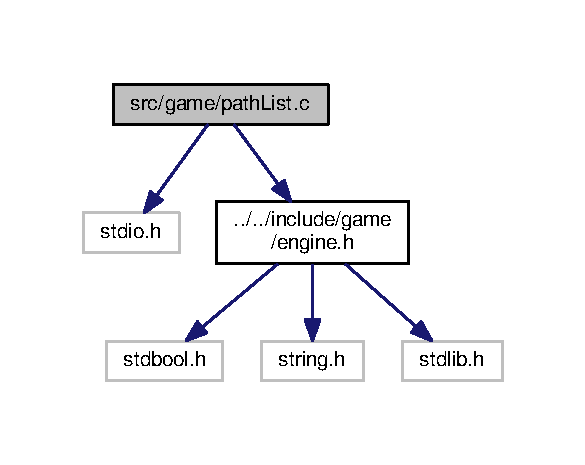
\includegraphics[width=281pt]{pathList_8c__incl}
\end{center}
\end{figure}
\subsection*{Classes}
\begin{DoxyCompactItemize}
\item 
struct \hyperlink{structelem}{elem}
\begin{DoxyCompactList}\small\item\em Représente une case de la grille. \end{DoxyCompactList}\end{DoxyCompactItemize}
\subsection*{Définitions de type}
\begin{DoxyCompactItemize}
\item 
\hypertarget{pathList_8c_a0ccaaf001e365f4e3ba830861612119a}{}typedef struct \hyperlink{structelem}{elem} \hyperlink{pathList_8c_a0ccaaf001e365f4e3ba830861612119a}{t\+\_\+tile}\label{pathList_8c_a0ccaaf001e365f4e3ba830861612119a}

\begin{DoxyCompactList}\small\item\em Définis la case. \end{DoxyCompactList}\end{DoxyCompactItemize}
\subsection*{Fonctions}
\begin{DoxyCompactItemize}
\item 
void \hyperlink{pathList_8c_ac694d579d04ee78ad2aa18f255272ed0}{init\+Path} (int n)
\begin{DoxyCompactList}\small\item\em Initialise le chemin. \end{DoxyCompactList}\item 
\hypertarget{pathList_8c_aca469a8527a0bc92e66306a1c8ada185}{}void \hyperlink{pathList_8c_aca469a8527a0bc92e66306a1c8ada185}{init\+Paths} ()\label{pathList_8c_aca469a8527a0bc92e66306a1c8ada185}

\begin{DoxyCompactList}\small\item\em Initialise les chemins. \end{DoxyCompactList}\item 
int \hyperlink{pathList_8c_a2aab13e3009ebe3949a32c10c03adcd8}{empty\+Path} (int n)
\begin{DoxyCompactList}\small\item\em Vérifie si un chemin est vide. \end{DoxyCompactList}\item 
int \hyperlink{pathList_8c_a4bcf1b8579c9a03c9070e33c77993426}{out\+Path} (int n)
\begin{DoxyCompactList}\small\item\em Vérifie si l\textquotesingle{}élément courant est hors liste. \end{DoxyCompactList}\item 
void \hyperlink{pathList_8c_af5f66b0e2d9ff7dd44fdd821bb9377cf}{path\+Head} (int n)
\begin{DoxyCompactList}\small\item\em Se met en tête du chemin. \end{DoxyCompactList}\item 
void \hyperlink{pathList_8c_a58814bcfb1182201bbecf88f839cd0f7}{path\+Tail} (int n)
\begin{DoxyCompactList}\small\item\em Se met en queue du chemin. \end{DoxyCompactList}\item 
void \hyperlink{pathList_8c_a2e1e62efbdb494f85de87088a068c916}{previous} (int n)
\begin{DoxyCompactList}\small\item\em Se positionne sur l\textquotesingle{}élément précédent. \end{DoxyCompactList}\item 
void \hyperlink{pathList_8c_ae29c8124809dc534b7ff12214d16183c}{next} (int n)
\begin{DoxyCompactList}\small\item\em Se positionne sur l\textquotesingle{}élémént suivant. \end{DoxyCompactList}\item 
void \hyperlink{pathList_8c_affe2967c536ca680e1389c746dc2d944}{get\+Tile} (int n, \hyperlink{structvector}{vector} $\ast$v, int $\ast$F)
\begin{DoxyCompactList}\small\item\em Récupère une case du chemin. \end{DoxyCompactList}\item 
\hyperlink{structvector}{vector} \hyperlink{pathList_8c_ae36257ead315faab602c58a4a2ae19fc}{get\+Current\+Node} (int n)
\begin{DoxyCompactList}\small\item\em Récupère le noeud ayant le plus petit F. \end{DoxyCompactList}\item 
void \hyperlink{pathList_8c_afac156c3a2eedf22deaae38595f95a65}{set\+Tile} (int n, \hyperlink{structvector}{vector} v, int F)
\begin{DoxyCompactList}\small\item\em Modifie les infos d\textquotesingle{}une case dans la liste. \end{DoxyCompactList}\item 
void \hyperlink{pathList_8c_acb403a99e156dd37be05e5d1245ca591}{erase\+Tile} (int n)
\begin{DoxyCompactList}\small\item\em Efface une case de la grille. \end{DoxyCompactList}\item 
void \hyperlink{pathList_8c_add77d77457e5c3b5e5e3ba1574e1e706}{to\+Right\+Path} (int n, \hyperlink{structvector}{vector} v, int F)
\begin{DoxyCompactList}\small\item\em Ajoute une case à droite. \end{DoxyCompactList}\item 
void \hyperlink{pathList_8c_afd17fd81ff6e16ee988340ae898ba362}{dump\+Path} (short nb\+List)
\begin{DoxyCompactList}\small\item\em Vide une liste. \end{DoxyCompactList}\item 
void \hyperlink{pathList_8c_a18154e93d817c730195d7fa04bd6c1d3}{dump\+All\+Paths} ()
\begin{DoxyCompactList}\small\item\em Vide toutes les listes. \end{DoxyCompactList}\item 
bool \hyperlink{pathList_8c_addf59bdd9af78dee4e241604e414ee57}{search\+Tile} (int n, \hyperlink{structvector}{vector} coord\+Tile)
\begin{DoxyCompactList}\small\item\em Cherche si un vecteur est présent dans la liste fermée ou ouverte. \end{DoxyCompactList}\item 
void \hyperlink{pathList_8c_a8c9ba5598845850e0fbaf8e3703b07e7}{add\+Close\+List} (\hyperlink{structvector}{vector} current, int F)
\begin{DoxyCompactList}\small\item\em Ajoute à la liste fermée. \end{DoxyCompactList}\item 
void \hyperlink{pathList_8c_a263a98f63b0badbcbb9dcb968cb04c00}{add\+Open\+List} (\hyperlink{structvector}{vector} current, int F)
\begin{DoxyCompactList}\small\item\em Ajoute à la liste ouverte. \end{DoxyCompactList}\end{DoxyCompactItemize}
\subsection*{Variables}
\begin{DoxyCompactItemize}
\item 
\hypertarget{pathList_8c_a21a7dd83d4282d5ba2d0be01a8b75964}{}\hyperlink{pathList_8c_a0ccaaf001e365f4e3ba830861612119a}{t\+\_\+tile} $\ast$ \hyperlink{pathList_8c_a21a7dd83d4282d5ba2d0be01a8b75964}{flag} \mbox{[}2\mbox{]}\label{pathList_8c_a21a7dd83d4282d5ba2d0be01a8b75964}

\begin{DoxyCompactList}\small\item\em Tableau de drapeaux. \end{DoxyCompactList}\item 
\hypertarget{pathList_8c_a791e2fe0ae92b02b3acda4f63c4b6056}{}\hyperlink{pathList_8c_a0ccaaf001e365f4e3ba830861612119a}{t\+\_\+tile} $\ast$ \hyperlink{pathList_8c_a791e2fe0ae92b02b3acda4f63c4b6056}{elem\+C} \mbox{[}2\mbox{]}\label{pathList_8c_a791e2fe0ae92b02b3acda4f63c4b6056}

\begin{DoxyCompactList}\small\item\em Tableau d\textquotesingle{}éléments courants. \end{DoxyCompactList}\end{DoxyCompactItemize}


\subsection{Description détaillée}
Listes de cases sur un chemin définis. 

\begin{DoxyAuthor}{Auteur}
Cousin Brandon Chaudemanche Ewen Biardeau Tristan 
\end{DoxyAuthor}
\begin{DoxyVersion}{Version}
v1.\+00 
\end{DoxyVersion}
\begin{DoxyDate}{Date}
18/12/2015 
\end{DoxyDate}


\subsection{Documentation des fonctions}
\hypertarget{pathList_8c_a8c9ba5598845850e0fbaf8e3703b07e7}{}\index{path\+List.\+c@{path\+List.\+c}!add\+Close\+List@{add\+Close\+List}}
\index{add\+Close\+List@{add\+Close\+List}!path\+List.\+c@{path\+List.\+c}}
\subsubsection[{add\+Close\+List}]{\setlength{\rightskip}{0pt plus 5cm}void add\+Close\+List (
\begin{DoxyParamCaption}
\item[{{\bf vector}}]{current, }
\item[{int}]{F}
\end{DoxyParamCaption}
)}\label{pathList_8c_a8c9ba5598845850e0fbaf8e3703b07e7}


Ajoute à la liste fermée. 

Ajoute la case à la liste fermée.


\begin{DoxyParams}{Paramètres}
{\em current} & Destination \\
\hline
{\em F} & Poids de la case \\
\hline
\end{DoxyParams}


Définition à la ligne 262 du fichier path\+List.\+c.

\hypertarget{pathList_8c_a263a98f63b0badbcbb9dcb968cb04c00}{}\index{path\+List.\+c@{path\+List.\+c}!add\+Open\+List@{add\+Open\+List}}
\index{add\+Open\+List@{add\+Open\+List}!path\+List.\+c@{path\+List.\+c}}
\subsubsection[{add\+Open\+List}]{\setlength{\rightskip}{0pt plus 5cm}void add\+Open\+List (
\begin{DoxyParamCaption}
\item[{{\bf vector}}]{current, }
\item[{int}]{F}
\end{DoxyParamCaption}
)}\label{pathList_8c_a263a98f63b0badbcbb9dcb968cb04c00}


Ajoute à la liste ouverte. 

Ajoute la case à la liste ouverte.


\begin{DoxyParams}{Paramètres}
{\em current} & Destination \\
\hline
{\em F} & Poids de la case \\
\hline
\end{DoxyParams}


Définition à la ligne 285 du fichier path\+List.\+c.

\hypertarget{pathList_8c_a18154e93d817c730195d7fa04bd6c1d3}{}\index{path\+List.\+c@{path\+List.\+c}!dump\+All\+Paths@{dump\+All\+Paths}}
\index{dump\+All\+Paths@{dump\+All\+Paths}!path\+List.\+c@{path\+List.\+c}}
\subsubsection[{dump\+All\+Paths}]{\setlength{\rightskip}{0pt plus 5cm}void dump\+All\+Paths (
\begin{DoxyParamCaption}
{}
\end{DoxyParamCaption}
)}\label{pathList_8c_a18154e93d817c730195d7fa04bd6c1d3}


Vide toutes les listes. 

Vide les chemins. 

Définition à la ligne 226 du fichier path\+List.\+c.

\hypertarget{pathList_8c_afd17fd81ff6e16ee988340ae898ba362}{}\index{path\+List.\+c@{path\+List.\+c}!dump\+Path@{dump\+Path}}
\index{dump\+Path@{dump\+Path}!path\+List.\+c@{path\+List.\+c}}
\subsubsection[{dump\+Path}]{\setlength{\rightskip}{0pt plus 5cm}void dump\+Path (
\begin{DoxyParamCaption}
\item[{short}]{nb\+List}
\end{DoxyParamCaption}
)}\label{pathList_8c_afd17fd81ff6e16ee988340ae898ba362}


Vide une liste. 

Vide le chemin.


\begin{DoxyParams}{Paramètres}
{\em nb\+List} & Numéro de la liste à vider \\
\hline
\end{DoxyParams}


Définition à la ligne 214 du fichier path\+List.\+c.

\hypertarget{pathList_8c_a2aab13e3009ebe3949a32c10c03adcd8}{}\index{path\+List.\+c@{path\+List.\+c}!empty\+Path@{empty\+Path}}
\index{empty\+Path@{empty\+Path}!path\+List.\+c@{path\+List.\+c}}
\subsubsection[{empty\+Path}]{\setlength{\rightskip}{0pt plus 5cm}int empty\+Path (
\begin{DoxyParamCaption}
\item[{int}]{n}
\end{DoxyParamCaption}
)}\label{pathList_8c_a2aab13e3009ebe3949a32c10c03adcd8}


Vérifie si un chemin est vide. 

Vérifie si chemin vide.


\begin{DoxyParams}{Paramètres}
{\em n} & Chemin \\
\hline
\end{DoxyParams}
\begin{DoxyReturn}{Renvoie}
Retourne le drapeau si pas vide 
\end{DoxyReturn}


Définition à la ligne 54 du fichier path\+List.\+c.

\hypertarget{pathList_8c_acb403a99e156dd37be05e5d1245ca591}{}\index{path\+List.\+c@{path\+List.\+c}!erase\+Tile@{erase\+Tile}}
\index{erase\+Tile@{erase\+Tile}!path\+List.\+c@{path\+List.\+c}}
\subsubsection[{erase\+Tile}]{\setlength{\rightskip}{0pt plus 5cm}void erase\+Tile (
\begin{DoxyParamCaption}
\item[{int}]{n}
\end{DoxyParamCaption}
)}\label{pathList_8c_acb403a99e156dd37be05e5d1245ca591}


Efface une case de la grille. 

Efface une case.


\begin{DoxyParams}{Paramètres}
{\em n} & Liste \\
\hline
\end{DoxyParams}


Définition à la ligne 170 du fichier path\+List.\+c.

\hypertarget{pathList_8c_ae36257ead315faab602c58a4a2ae19fc}{}\index{path\+List.\+c@{path\+List.\+c}!get\+Current\+Node@{get\+Current\+Node}}
\index{get\+Current\+Node@{get\+Current\+Node}!path\+List.\+c@{path\+List.\+c}}
\subsubsection[{get\+Current\+Node}]{\setlength{\rightskip}{0pt plus 5cm}{\bf vector} get\+Current\+Node (
\begin{DoxyParamCaption}
\item[{int}]{n}
\end{DoxyParamCaption}
)}\label{pathList_8c_ae36257ead315faab602c58a4a2ae19fc}


Récupère le noeud ayant le plus petit F. 

Récupère la case ayant le plus petit poids.


\begin{DoxyParams}{Paramètres}
{\em n} & Liste dans laquelle chercher \\
\hline
\end{DoxyParams}


Définition à la ligne 130 du fichier path\+List.\+c.

\hypertarget{pathList_8c_affe2967c536ca680e1389c746dc2d944}{}\index{path\+List.\+c@{path\+List.\+c}!get\+Tile@{get\+Tile}}
\index{get\+Tile@{get\+Tile}!path\+List.\+c@{path\+List.\+c}}
\subsubsection[{get\+Tile}]{\setlength{\rightskip}{0pt plus 5cm}void get\+Tile (
\begin{DoxyParamCaption}
\item[{int}]{n, }
\item[{{\bf vector} $\ast$}]{v, }
\item[{int $\ast$}]{F}
\end{DoxyParamCaption}
)}\label{pathList_8c_affe2967c536ca680e1389c746dc2d944}


Récupère une case du chemin. 

Récupère la valeur d\textquotesingle{}une case.


\begin{DoxyParams}{Paramètres}
{\em n} & Chemin \\
\hline
{\em v} & Position de la case \\
\hline
{\em F} & Poids de la case \\
\hline
\end{DoxyParams}


Définition à la ligne 117 du fichier path\+List.\+c.

\hypertarget{pathList_8c_ac694d579d04ee78ad2aa18f255272ed0}{}\index{path\+List.\+c@{path\+List.\+c}!init\+Path@{init\+Path}}
\index{init\+Path@{init\+Path}!path\+List.\+c@{path\+List.\+c}}
\subsubsection[{init\+Path}]{\setlength{\rightskip}{0pt plus 5cm}void init\+Path (
\begin{DoxyParamCaption}
\item[{int}]{n}
\end{DoxyParamCaption}
)}\label{pathList_8c_ac694d579d04ee78ad2aa18f255272ed0}


Initialise le chemin. 


\begin{DoxyParams}{Paramètres}
{\em n} & Chemin \\
\hline
\end{DoxyParams}


Définition à la ligne 31 du fichier path\+List.\+c.

\hypertarget{pathList_8c_ae29c8124809dc534b7ff12214d16183c}{}\index{path\+List.\+c@{path\+List.\+c}!next@{next}}
\index{next@{next}!path\+List.\+c@{path\+List.\+c}}
\subsubsection[{next}]{\setlength{\rightskip}{0pt plus 5cm}void next (
\begin{DoxyParamCaption}
\item[{int}]{n}
\end{DoxyParamCaption}
)}\label{pathList_8c_ae29c8124809dc534b7ff12214d16183c}


Se positionne sur l\textquotesingle{}élémént suivant. 

Se positionne sur l\textquotesingle{}élément suivant.


\begin{DoxyParams}{Paramètres}
{\em n} & Chemin \\
\hline
\end{DoxyParams}


Définition à la ligne 105 du fichier path\+List.\+c.

\hypertarget{pathList_8c_a4bcf1b8579c9a03c9070e33c77993426}{}\index{path\+List.\+c@{path\+List.\+c}!out\+Path@{out\+Path}}
\index{out\+Path@{out\+Path}!path\+List.\+c@{path\+List.\+c}}
\subsubsection[{out\+Path}]{\setlength{\rightskip}{0pt plus 5cm}int out\+Path (
\begin{DoxyParamCaption}
\item[{int}]{n}
\end{DoxyParamCaption}
)}\label{pathList_8c_a4bcf1b8579c9a03c9070e33c77993426}


Vérifie si l\textquotesingle{}élément courant est hors liste. 

Vérifie si l\textquotesingle{}élément courant est en dehors de la liste.


\begin{DoxyParams}{Paramètres}
{\em n} & Liste \\
\hline
\end{DoxyParams}
\begin{DoxyReturn}{Renvoie}
Retourne l\textquotesingle{}élément courant si pas hors liste 
\end{DoxyReturn}


Définition à la ligne 65 du fichier path\+List.\+c.

\hypertarget{pathList_8c_af5f66b0e2d9ff7dd44fdd821bb9377cf}{}\index{path\+List.\+c@{path\+List.\+c}!path\+Head@{path\+Head}}
\index{path\+Head@{path\+Head}!path\+List.\+c@{path\+List.\+c}}
\subsubsection[{path\+Head}]{\setlength{\rightskip}{0pt plus 5cm}void path\+Head (
\begin{DoxyParamCaption}
\item[{int}]{n}
\end{DoxyParamCaption}
)}\label{pathList_8c_af5f66b0e2d9ff7dd44fdd821bb9377cf}


Se met en tête du chemin. 

Se met en tête de la liste.


\begin{DoxyParams}{Paramètres}
{\em n} & Chemin \\
\hline
\end{DoxyParams}


Définition à la ligne 75 du fichier path\+List.\+c.

\hypertarget{pathList_8c_a58814bcfb1182201bbecf88f839cd0f7}{}\index{path\+List.\+c@{path\+List.\+c}!path\+Tail@{path\+Tail}}
\index{path\+Tail@{path\+Tail}!path\+List.\+c@{path\+List.\+c}}
\subsubsection[{path\+Tail}]{\setlength{\rightskip}{0pt plus 5cm}void path\+Tail (
\begin{DoxyParamCaption}
\item[{int}]{n}
\end{DoxyParamCaption}
)}\label{pathList_8c_a58814bcfb1182201bbecf88f839cd0f7}


Se met en queue du chemin. 

Se met en queue de la liste.


\begin{DoxyParams}{Paramètres}
{\em n} & Chemin \\
\hline
\end{DoxyParams}


Définition à la ligne 85 du fichier path\+List.\+c.

\hypertarget{pathList_8c_a2e1e62efbdb494f85de87088a068c916}{}\index{path\+List.\+c@{path\+List.\+c}!previous@{previous}}
\index{previous@{previous}!path\+List.\+c@{path\+List.\+c}}
\subsubsection[{previous}]{\setlength{\rightskip}{0pt plus 5cm}void previous (
\begin{DoxyParamCaption}
\item[{int}]{n}
\end{DoxyParamCaption}
)}\label{pathList_8c_a2e1e62efbdb494f85de87088a068c916}


Se positionne sur l\textquotesingle{}élément précédent. 


\begin{DoxyParams}{Paramètres}
{\em n} & Chemin \\
\hline
\end{DoxyParams}


Définition à la ligne 95 du fichier path\+List.\+c.

\hypertarget{pathList_8c_addf59bdd9af78dee4e241604e414ee57}{}\index{path\+List.\+c@{path\+List.\+c}!search\+Tile@{search\+Tile}}
\index{search\+Tile@{search\+Tile}!path\+List.\+c@{path\+List.\+c}}
\subsubsection[{search\+Tile}]{\setlength{\rightskip}{0pt plus 5cm}bool search\+Tile (
\begin{DoxyParamCaption}
\item[{int}]{n, }
\item[{{\bf vector}}]{coord\+Tile}
\end{DoxyParamCaption}
)}\label{pathList_8c_addf59bdd9af78dee4e241604e414ee57}


Cherche si un vecteur est présent dans la liste fermée ou ouverte. 

Cherche une case.


\begin{DoxyParams}{Paramètres}
{\em n} & Liste \\
\hline
{\em coord\+Tile} & Position de la case \\
\hline
\end{DoxyParams}


Définition à la ligne 239 du fichier path\+List.\+c.

\hypertarget{pathList_8c_afac156c3a2eedf22deaae38595f95a65}{}\index{path\+List.\+c@{path\+List.\+c}!set\+Tile@{set\+Tile}}
\index{set\+Tile@{set\+Tile}!path\+List.\+c@{path\+List.\+c}}
\subsubsection[{set\+Tile}]{\setlength{\rightskip}{0pt plus 5cm}void set\+Tile (
\begin{DoxyParamCaption}
\item[{int}]{n, }
\item[{{\bf vector}}]{v, }
\item[{int}]{F}
\end{DoxyParamCaption}
)}\label{pathList_8c_afac156c3a2eedf22deaae38595f95a65}


Modifie les infos d\textquotesingle{}une case dans la liste. 

Modifie la valeur d\textquotesingle{}une case.


\begin{DoxyParams}{Paramètres}
{\em n} & Liste \\
\hline
{\em v} & Nouvelle position \\
\hline
{\em F} & Nouveau poids \\
\hline
\end{DoxyParams}


Définition à la ligne 157 du fichier path\+List.\+c.

\hypertarget{pathList_8c_add77d77457e5c3b5e5e3ba1574e1e706}{}\index{path\+List.\+c@{path\+List.\+c}!to\+Right\+Path@{to\+Right\+Path}}
\index{to\+Right\+Path@{to\+Right\+Path}!path\+List.\+c@{path\+List.\+c}}
\subsubsection[{to\+Right\+Path}]{\setlength{\rightskip}{0pt plus 5cm}void to\+Right\+Path (
\begin{DoxyParamCaption}
\item[{int}]{n, }
\item[{{\bf vector}}]{v, }
\item[{int}]{F}
\end{DoxyParamCaption}
)}\label{pathList_8c_add77d77457e5c3b5e5e3ba1574e1e706}


Ajoute une case à droite. 


\begin{DoxyParams}{Paramètres}
{\em n} & Liste \\
\hline
{\em v} & Position à ajouter \\
\hline
{\em F} & Poids à ajouter \\
\hline
\end{DoxyParams}


Définition à la ligne 191 du fichier path\+List.\+c.


\hypertarget{pawns_8c}{}\section{Référence du fichier src/game/pawns.c}
\label{pawns_8c}\index{src/game/pawns.\+c@{src/game/pawns.\+c}}


Gestion des pions.  


{\ttfamily \#include $<$stdio.\+h$>$}\\*
{\ttfamily \#include $<$stdarg.\+h$>$}\\*
{\ttfamily \#include \char`\"{}../../include/game/engine.\+h\char`\"{}}\\*
{\ttfamily \#include \char`\"{}../../include/game/listes.\+h\char`\"{}}\\*
{\ttfamily \#include \char`\"{}../../include/controller/terminal.\+h\char`\"{}}\\*
{\ttfamily \#include \char`\"{}../../include/controller/manage\+String.\+h\char`\"{}}\\*
Graphe des dépendances par inclusion de pawns.\+c\+:\nopagebreak
\begin{figure}[H]
\begin{center}
\leavevmode
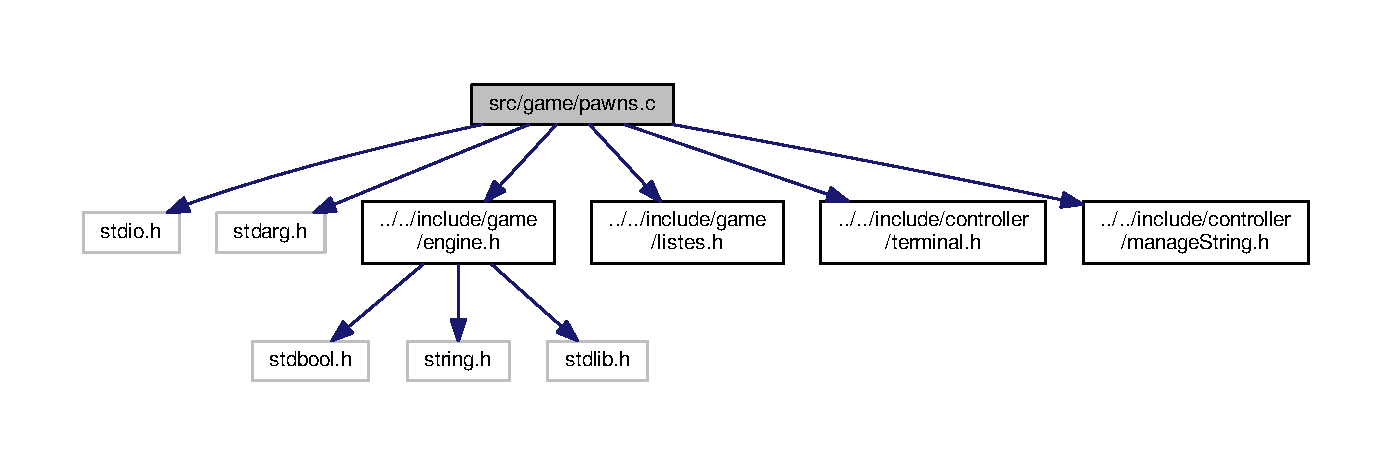
\includegraphics[width=350pt]{pawns_8c__incl}
\end{center}
\end{figure}
\subsection*{Fonctions}
\begin{DoxyCompactItemize}
\item 
void \hyperlink{pawns_8c_aeea3cc5ad26ccda694a140445ad067c4}{init\+Pawn} (\hyperlink{structunit}{unit} $\ast$pawn)
\begin{DoxyCompactList}\small\item\em Initialise un pion. \end{DoxyCompactList}\item 
bool \hyperlink{pawns_8c_ae83822f14210ca3bff153d900ea2dc58}{check\+Pawn} (\hyperlink{structunit}{unit} $\ast$pawn)
\begin{DoxyCompactList}\small\item\em Vérifie que le pion est correct. \end{DoxyCompactList}\item 
void \hyperlink{pawns_8c_ab64bdacff221584d1ffbae4dd7f19ce8}{create\+Pawn} (int nb\+Params, \hyperlink{engine_8h_af7667555c2dcfbdd55ec3e9dd6a907ba}{unit\+Name} name,...)
\begin{DoxyCompactList}\small\item\em Crée un pion pour le jeu. \end{DoxyCompactList}\item 
void \hyperlink{pawns_8c_af3226144d32d485e7e1362861b69ca11}{make\+Pawns} ()
\begin{DoxyCompactList}\small\item\em Crée tout les pions utiles au jeu. \end{DoxyCompactList}\end{DoxyCompactItemize}
\subsection*{Variables}
\begin{DoxyCompactItemize}
\item 
\hyperlink{structunit}{unit} $\ast$ \hyperlink{pawns_8c_a0ec7c043ade24d330b48f393097f140f}{pawns} = N\+U\+L\+L
\begin{DoxyCompactList}\small\item\em Pions initialisés avec leur valeurs. \end{DoxyCompactList}\item 
\hypertarget{pawns_8c_a202e0786b273cb3b8e8cbe51ea8e3d1a}{}int \hyperlink{pawns_8c_a202e0786b273cb3b8e8cbe51ea8e3d1a}{size\+Pawns} = 0\label{pawns_8c_a202e0786b273cb3b8e8cbe51ea8e3d1a}

\begin{DoxyCompactList}\small\item\em Nombre de pions. \end{DoxyCompactList}\end{DoxyCompactItemize}


\subsection{Description détaillée}
Gestion des pions. 

\begin{DoxyAuthor}{Auteur}
Cousin Brandon Chaudemanche Ewen Biardeau Tristan 
\end{DoxyAuthor}
\begin{DoxyVersion}{Version}
v1.\+00 
\end{DoxyVersion}
\begin{DoxyDate}{Date}
18/12/2015 
\end{DoxyDate}


\subsection{Documentation des fonctions}
\hypertarget{pawns_8c_ae83822f14210ca3bff153d900ea2dc58}{}\index{pawns.\+c@{pawns.\+c}!check\+Pawn@{check\+Pawn}}
\index{check\+Pawn@{check\+Pawn}!pawns.\+c@{pawns.\+c}}
\subsubsection[{check\+Pawn}]{\setlength{\rightskip}{0pt plus 5cm}bool check\+Pawn (
\begin{DoxyParamCaption}
\item[{{\bf unit} $\ast$}]{pawn}
\end{DoxyParamCaption}
)}\label{pawns_8c_ae83822f14210ca3bff153d900ea2dc58}


Vérifie que le pion est correct. 


\begin{DoxyParams}{Paramètres}
{\em pawn} & Pion à vérifier \\
\hline
\end{DoxyParams}
\begin{DoxyReturn}{Renvoie}
Retourne vrai si le pion est correct 
\end{DoxyReturn}


Définition à la ligne 37 du fichier pawns.\+c.

\hypertarget{pawns_8c_ab64bdacff221584d1ffbae4dd7f19ce8}{}\index{pawns.\+c@{pawns.\+c}!create\+Pawn@{create\+Pawn}}
\index{create\+Pawn@{create\+Pawn}!pawns.\+c@{pawns.\+c}}
\subsubsection[{create\+Pawn}]{\setlength{\rightskip}{0pt plus 5cm}void create\+Pawn (
\begin{DoxyParamCaption}
\item[{int}]{nb\+Params, }
\item[{{\bf unit\+Name}}]{name, }
\item[{}]{...}
\end{DoxyParamCaption}
)}\label{pawns_8c_ab64bdacff221584d1ffbae4dd7f19ce8}


Crée un pion pour le jeu. 


\begin{DoxyParams}{Paramètres}
{\em nb\+Params} & Nombre de stats pour le pion \\
\hline
{\em name} & Nom du pion \\
\hline
\end{DoxyParams}


Définition à la ligne 51 du fichier pawns.\+c.

\hypertarget{pawns_8c_aeea3cc5ad26ccda694a140445ad067c4}{}\index{pawns.\+c@{pawns.\+c}!init\+Pawn@{init\+Pawn}}
\index{init\+Pawn@{init\+Pawn}!pawns.\+c@{pawns.\+c}}
\subsubsection[{init\+Pawn}]{\setlength{\rightskip}{0pt plus 5cm}void init\+Pawn (
\begin{DoxyParamCaption}
\item[{{\bf unit} $\ast$}]{pawn}
\end{DoxyParamCaption}
)}\label{pawns_8c_aeea3cc5ad26ccda694a140445ad067c4}


Initialise un pion. 


\begin{DoxyParams}{Paramètres}
{\em pawn} & Pion à initialiser \\
\hline
\end{DoxyParams}


Définition à la ligne 23 du fichier pawns.\+c.

\hypertarget{pawns_8c_af3226144d32d485e7e1362861b69ca11}{}\index{pawns.\+c@{pawns.\+c}!make\+Pawns@{make\+Pawns}}
\index{make\+Pawns@{make\+Pawns}!pawns.\+c@{pawns.\+c}}
\subsubsection[{make\+Pawns}]{\setlength{\rightskip}{0pt plus 5cm}void make\+Pawns (
\begin{DoxyParamCaption}
{}
\end{DoxyParamCaption}
)}\label{pawns_8c_af3226144d32d485e7e1362861b69ca11}


Crée tout les pions utiles au jeu. 

Crée les pions. 

Définition à la ligne 109 du fichier pawns.\+c.



\subsection{Documentation des variables}
\hypertarget{pawns_8c_a0ec7c043ade24d330b48f393097f140f}{}\index{pawns.\+c@{pawns.\+c}!pawns@{pawns}}
\index{pawns@{pawns}!pawns.\+c@{pawns.\+c}}
\subsubsection[{pawns}]{\setlength{\rightskip}{0pt plus 5cm}{\bf unit}$\ast$ pawns = N\+U\+L\+L}\label{pawns_8c_a0ec7c043ade24d330b48f393097f140f}


Pions initialisés avec leur valeurs. 

Tableaux des pions. 

Définition à la ligne 16 du fichier pawns.\+c.


\hypertarget{turn_8c}{}\section{Référence du fichier src/game/turn.c}
\label{turn_8c}\index{src/game/turn.\+c@{src/game/turn.\+c}}


Gestion des tours.  


{\ttfamily \#include $<$time.\+h$>$}\\*
{\ttfamily \#include $<$stdio.\+h$>$}\\*
{\ttfamily \#include $<$signal.\+h$>$}\\*
{\ttfamily \#include \char`\"{}../../include/game/engine.\+h\char`\"{}}\\*
{\ttfamily \#include \char`\"{}../../include/game/pawns.\+h\char`\"{}}\\*
{\ttfamily \#include \char`\"{}../../include/game/turn.\+h\char`\"{}}\\*
{\ttfamily \#include \char`\"{}../../include/game/listes.\+h\char`\"{}}\\*
{\ttfamily \#include \char`\"{}../../include/display/grid.\+h\char`\"{}}\\*
{\ttfamily \#include \char`\"{}../../include/display/menu.\+h\char`\"{}}\\*
{\ttfamily \#include \char`\"{}../../include/controller/terminal.\+h\char`\"{}}\\*
{\ttfamily \#include \char`\"{}../../include/controller/manage\+Signal.\+h\char`\"{}}\\*
{\ttfamily \#include \char`\"{}../../include/controller/manage\+String.\+h\char`\"{}}\\*
{\ttfamily \#include \char`\"{}../../include/units/unit.\+h\char`\"{}}\\*
Graphe des dépendances par inclusion de turn.\+c\+:\nopagebreak
\begin{figure}[H]
\begin{center}
\leavevmode
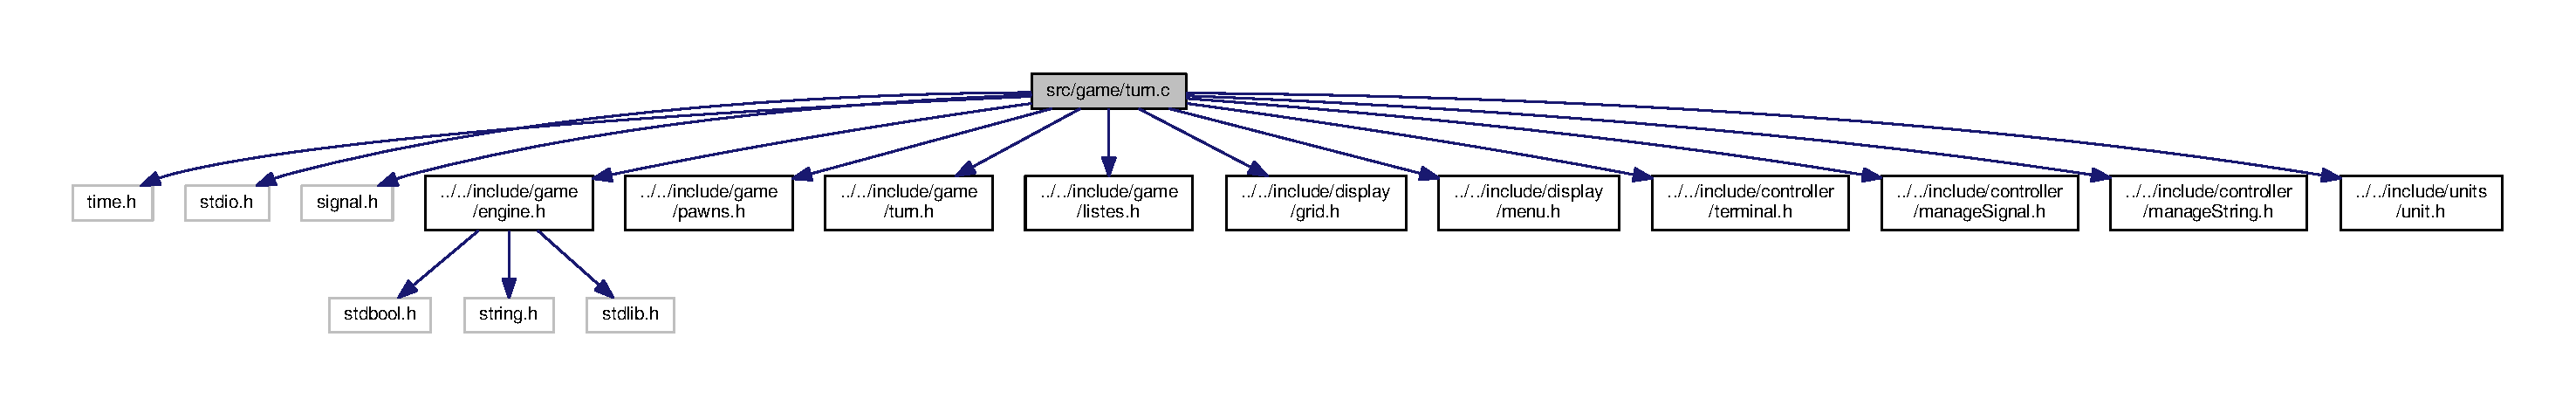
\includegraphics[width=350pt]{turn_8c__incl}
\end{center}
\end{figure}
\subsection*{Fonctions}
\begin{DoxyCompactItemize}
\item 
\hypertarget{turn_8c_af833187c9cee5a9fc025b1d37e4ea473}{}int \hyperlink{turn_8c_af833187c9cee5a9fc025b1d37e4ea473}{start\+Turn} ()\label{turn_8c_af833187c9cee5a9fc025b1d37e4ea473}

\begin{DoxyCompactList}\small\item\em Débute le tour du joueur. \end{DoxyCompactList}\item 
int \hyperlink{turn_8c_a9b3f364f20175067c0349246c843953b}{end\+Turn} (time\+\_\+t start, int total\+Time)
\begin{DoxyCompactList}\small\item\em Renvoie le temps restant avant la fin du tour. \end{DoxyCompactList}\item 
void \hyperlink{turn_8c_a9d6b655a52683afe2f4cb87e3f64bc2e}{change\+Direction} ()
\begin{DoxyCompactList}\small\item\em Change la direction de l\textquotesingle{}unité \end{DoxyCompactList}\item 
void \hyperlink{turn_8c_a0d63b19dd2910e04bc114a4572276601}{play\+Attack} ()
\begin{DoxyCompactList}\small\item\em Jouer une attaque. \end{DoxyCompactList}\item 
void \hyperlink{turn_8c_af6050b30e522cb4218786756c972d804}{play\+Move} ()
\begin{DoxyCompactList}\small\item\em Jouer un mouvement. \end{DoxyCompactList}\item 
void \hyperlink{turn_8c_ab4e21eee8105ce3f15cb490ce17225e8}{pass\+Turn} ()
\begin{DoxyCompactList}\small\item\em Passer tour. \end{DoxyCompactList}\item 
bool \hyperlink{turn_8c_a2c1ed39b34b58552a4cba52a3f832d14}{has\+Play} ()
\begin{DoxyCompactList}\small\item\em Définis si le joueur a joué \end{DoxyCompactList}\item 
\hypertarget{turn_8c_a5032490db7416ec2004861d51acda9e2}{}void \hyperlink{turn_8c_a5032490db7416ec2004861d51acda9e2}{surrender} ()\label{turn_8c_a5032490db7416ec2004861d51acda9e2}

\begin{DoxyCompactList}\small\item\em Abandonne la partie. \end{DoxyCompactList}\item 
void \hyperlink{turn_8c_aa39775041a9e8da2a156b4f75d646cdc}{set\+Action} (int time\+Left)
\begin{DoxyCompactList}\small\item\em Définis si l\textquotesingle{}action est à prendre en compte. \end{DoxyCompactList}\item 
void \hyperlink{turn_8c_af77ebb54a900a2ef4a15ea354ff60f85}{play\+Turn} ()
\begin{DoxyCompactList}\small\item\em Jouer un tour. \end{DoxyCompactList}\end{DoxyCompactItemize}
\subsection*{Variables}
\begin{DoxyCompactItemize}
\item 
\hypertarget{turn_8c_a5849a680495b395c75c2269657d5d4a5}{}int \hyperlink{turn_8c_a5849a680495b395c75c2269657d5d4a5}{has\+Moved} = 0\label{turn_8c_a5849a680495b395c75c2269657d5d4a5}

\begin{DoxyCompactList}\small\item\em Joueur a joué \end{DoxyCompactList}\item 
\hypertarget{turn_8c_a1fa6b4cfe1a42f3d14c8701782a8ae6f}{}int \hyperlink{turn_8c_a1fa6b4cfe1a42f3d14c8701782a8ae6f}{has\+Attacked} = 0\label{turn_8c_a1fa6b4cfe1a42f3d14c8701782a8ae6f}

\begin{DoxyCompactList}\small\item\em Joueur a attaqué \end{DoxyCompactList}\item 
\hypertarget{turn_8c_a776a08ce69ed60e7178f5fab585b5936}{}int \hyperlink{turn_8c_a776a08ce69ed60e7178f5fab585b5936}{has\+Passed} = 0\label{turn_8c_a776a08ce69ed60e7178f5fab585b5936}

\begin{DoxyCompactList}\small\item\em Joueur a passé son tour. \end{DoxyCompactList}\item 
\hypertarget{turn_8c_ab28ae3d21446f3eb01eeeab3002ad942}{}int \hyperlink{turn_8c_ab28ae3d21446f3eb01eeeab3002ad942}{has\+Surrender} = 0\label{turn_8c_ab28ae3d21446f3eb01eeeab3002ad942}

\begin{DoxyCompactList}\small\item\em Joueur a abandonné la partie. \end{DoxyCompactList}\end{DoxyCompactItemize}


\subsection{Description détaillée}
Gestion des tours. 

\begin{DoxyAuthor}{Auteur}
Cousin Brandon Chaudemanche Ewen Biardeau Tristan 
\end{DoxyAuthor}
\begin{DoxyVersion}{Version}
v1.\+00 
\end{DoxyVersion}
\begin{DoxyDate}{Date}
18/12/2015 
\end{DoxyDate}


\subsection{Documentation des fonctions}
\hypertarget{turn_8c_a9d6b655a52683afe2f4cb87e3f64bc2e}{}\index{turn.\+c@{turn.\+c}!change\+Direction@{change\+Direction}}
\index{change\+Direction@{change\+Direction}!turn.\+c@{turn.\+c}}
\subsubsection[{change\+Direction}]{\setlength{\rightskip}{0pt plus 5cm}void change\+Direction (
\begin{DoxyParamCaption}
{}
\end{DoxyParamCaption}
)}\label{turn_8c_a9d6b655a52683afe2f4cb87e3f64bc2e}


Change la direction de l\textquotesingle{}unité 

Change la direction. 

Définition à la ligne 57 du fichier turn.\+c.

\hypertarget{turn_8c_a9b3f364f20175067c0349246c843953b}{}\index{turn.\+c@{turn.\+c}!end\+Turn@{end\+Turn}}
\index{end\+Turn@{end\+Turn}!turn.\+c@{turn.\+c}}
\subsubsection[{end\+Turn}]{\setlength{\rightskip}{0pt plus 5cm}int end\+Turn (
\begin{DoxyParamCaption}
\item[{time\+\_\+t}]{start, }
\item[{int}]{total\+Time}
\end{DoxyParamCaption}
)}\label{turn_8c_a9b3f364f20175067c0349246c843953b}


Renvoie le temps restant avant la fin du tour. 


\begin{DoxyParams}{Paramètres}
{\em start} & Temps de début du tour \\
\hline
{\em total\+Time} & Temps total du tour \\
\hline
\end{DoxyParams}


Définition à la ligne 44 du fichier turn.\+c.

\hypertarget{turn_8c_a2c1ed39b34b58552a4cba52a3f832d14}{}\index{turn.\+c@{turn.\+c}!has\+Play@{has\+Play}}
\index{has\+Play@{has\+Play}!turn.\+c@{turn.\+c}}
\subsubsection[{has\+Play}]{\setlength{\rightskip}{0pt plus 5cm}bool has\+Play (
\begin{DoxyParamCaption}
{}
\end{DoxyParamCaption}
)}\label{turn_8c_a2c1ed39b34b58552a4cba52a3f832d14}


Définis si le joueur a joué 

Vérifie si une action a été effectuée.

\begin{DoxyReturn}{Renvoie}
Retourne vrai si le joueur a joué sinon faux 
\end{DoxyReturn}


Définition à la ligne 245 du fichier turn.\+c.

\hypertarget{turn_8c_ab4e21eee8105ce3f15cb490ce17225e8}{}\index{turn.\+c@{turn.\+c}!pass\+Turn@{pass\+Turn}}
\index{pass\+Turn@{pass\+Turn}!turn.\+c@{turn.\+c}}
\subsubsection[{pass\+Turn}]{\setlength{\rightskip}{0pt plus 5cm}void pass\+Turn (
\begin{DoxyParamCaption}
{}
\end{DoxyParamCaption}
)}\label{turn_8c_ab4e21eee8105ce3f15cb490ce17225e8}


Passer tour. 

Passe le tour. 

Définition à la ligne 235 du fichier turn.\+c.

\hypertarget{turn_8c_a0d63b19dd2910e04bc114a4572276601}{}\index{turn.\+c@{turn.\+c}!play\+Attack@{play\+Attack}}
\index{play\+Attack@{play\+Attack}!turn.\+c@{turn.\+c}}
\subsubsection[{play\+Attack}]{\setlength{\rightskip}{0pt plus 5cm}void play\+Attack (
\begin{DoxyParamCaption}
{}
\end{DoxyParamCaption}
)}\label{turn_8c_a0d63b19dd2910e04bc114a4572276601}


Jouer une attaque. 

Joue une attaque. 

Définition à la ligne 104 du fichier turn.\+c.

\hypertarget{turn_8c_af6050b30e522cb4218786756c972d804}{}\index{turn.\+c@{turn.\+c}!play\+Move@{play\+Move}}
\index{play\+Move@{play\+Move}!turn.\+c@{turn.\+c}}
\subsubsection[{play\+Move}]{\setlength{\rightskip}{0pt plus 5cm}void play\+Move (
\begin{DoxyParamCaption}
{}
\end{DoxyParamCaption}
)}\label{turn_8c_af6050b30e522cb4218786756c972d804}


Jouer un mouvement. 

Joue une mouvement. 

Définition à la ligne 177 du fichier turn.\+c.

\hypertarget{turn_8c_af77ebb54a900a2ef4a15ea354ff60f85}{}\index{turn.\+c@{turn.\+c}!play\+Turn@{play\+Turn}}
\index{play\+Turn@{play\+Turn}!turn.\+c@{turn.\+c}}
\subsubsection[{play\+Turn}]{\setlength{\rightskip}{0pt plus 5cm}void play\+Turn (
\begin{DoxyParamCaption}
{}
\end{DoxyParamCaption}
)}\label{turn_8c_af77ebb54a900a2ef4a15ea354ff60f85}


Jouer un tour. 

Joue un tour. 

Définition à la ligne 272 du fichier turn.\+c.

\hypertarget{turn_8c_aa39775041a9e8da2a156b4f75d646cdc}{}\index{turn.\+c@{turn.\+c}!set\+Action@{set\+Action}}
\index{set\+Action@{set\+Action}!turn.\+c@{turn.\+c}}
\subsubsection[{set\+Action}]{\setlength{\rightskip}{0pt plus 5cm}void set\+Action (
\begin{DoxyParamCaption}
\item[{int}]{time\+Left}
\end{DoxyParamCaption}
)}\label{turn_8c_aa39775041a9e8da2a156b4f75d646cdc}


Définis si l\textquotesingle{}action est à prendre en compte. 


\begin{DoxyParams}{Paramètres}
{\em time\+Left} & Temps restant pour le tour \\
\hline
\end{DoxyParams}


Définition à la ligne 261 du fichier turn.\+c.


\hypertarget{main_8c}{}\section{Référence du fichier src/main.c}
\label{main_8c}\index{src/main.\+c@{src/main.\+c}}


Programme principal.  


{\ttfamily \#include $<$stdio.\+h$>$}\\*
{\ttfamily \#include $<$signal.\+h$>$}\\*
{\ttfamily \#include $<$time.\+h$>$}\\*
{\ttfamily \#include \char`\"{}../include/game/engine.\+h\char`\"{}}\\*
{\ttfamily \#include \char`\"{}../include/game/pawns.\+h\char`\"{}}\\*
{\ttfamily \#include \char`\"{}../include/display/grid.\+h\char`\"{}}\\*
{\ttfamily \#include \char`\"{}../include/display/menu.\+h\char`\"{}}\\*
{\ttfamily \#include \char`\"{}../include/controller/manage\+String.\+h\char`\"{}}\\*
{\ttfamily \#include \char`\"{}../include/controller/manage\+Signal.\+h\char`\"{}}\\*
{\ttfamily \#include \char`\"{}../include/game/listes.\+h\char`\"{}}\\*
Graphe des dépendances par inclusion de main.\+c\+:\nopagebreak
\begin{figure}[H]
\begin{center}
\leavevmode
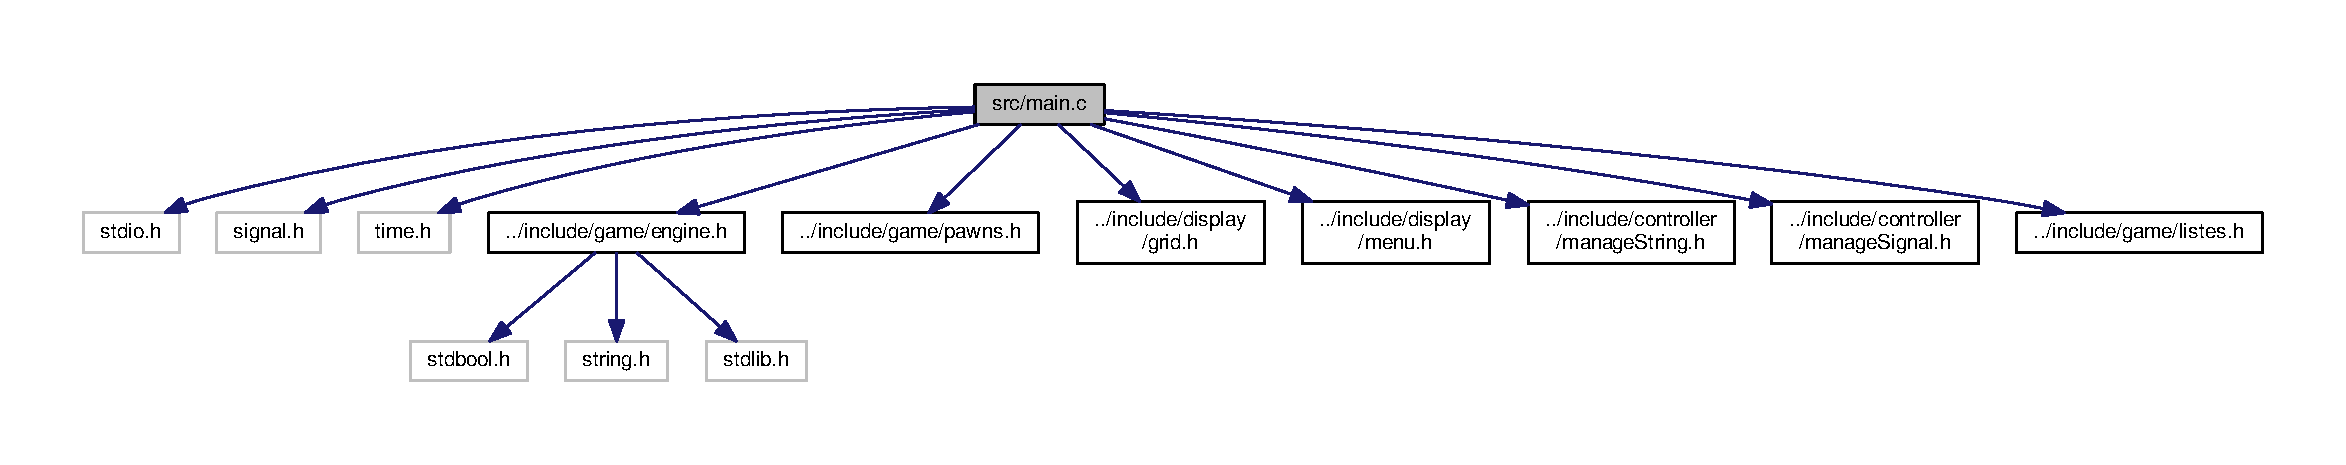
\includegraphics[width=350pt]{main_8c__incl}
\end{center}
\end{figure}
\subsection*{Fonctions}
\begin{DoxyCompactItemize}
\item 
\hypertarget{main_8c_ae66f6b31b5ad750f1fe042a706a4e3d4}{}int \hyperlink{main_8c_ae66f6b31b5ad750f1fe042a706a4e3d4}{main} ()\label{main_8c_ae66f6b31b5ad750f1fe042a706a4e3d4}

\begin{DoxyCompactList}\small\item\em Programme principal. \end{DoxyCompactList}\end{DoxyCompactItemize}


\subsection{Description détaillée}
Programme principal. 

\begin{DoxyAuthor}{Auteur}
Cousin Brandon Chaudemanche Ewen Biardeau Tristan 
\end{DoxyAuthor}
\begin{DoxyVersion}{Version}
v1.\+00 
\end{DoxyVersion}
\begin{DoxyDate}{Date}
18/12/2015 
\end{DoxyDate}

\hypertarget{unit_8c}{}\section{Référence du fichier src/units/unit.c}
\label{unit_8c}\index{src/units/unit.\+c@{src/units/unit.\+c}}


Gestion des unités.  


{\ttfamily \#include $<$stdio.\+h$>$}\\*
{\ttfamily \#include $<$math.\+h$>$}\\*
{\ttfamily \#include \char`\"{}../../include/game/engine.\+h\char`\"{}}\\*
{\ttfamily \#include \char`\"{}../../include/game/pawns.\+h\char`\"{}}\\*
{\ttfamily \#include \char`\"{}../../include/game/listes.\+h\char`\"{}}\\*
{\ttfamily \#include \char`\"{}../../include/display/grid.\+h\char`\"{}}\\*
{\ttfamily \#include \char`\"{}../../include/controller/terminal.\+h\char`\"{}}\\*
{\ttfamily \#include \char`\"{}../../include/controller/manage\+String.\+h\char`\"{}}\\*
{\ttfamily \#include \char`\"{}../../include/units/unit.\+h\char`\"{}}\\*
Graphe des dépendances par inclusion de unit.\+c\+:\nopagebreak
\begin{figure}[H]
\begin{center}
\leavevmode
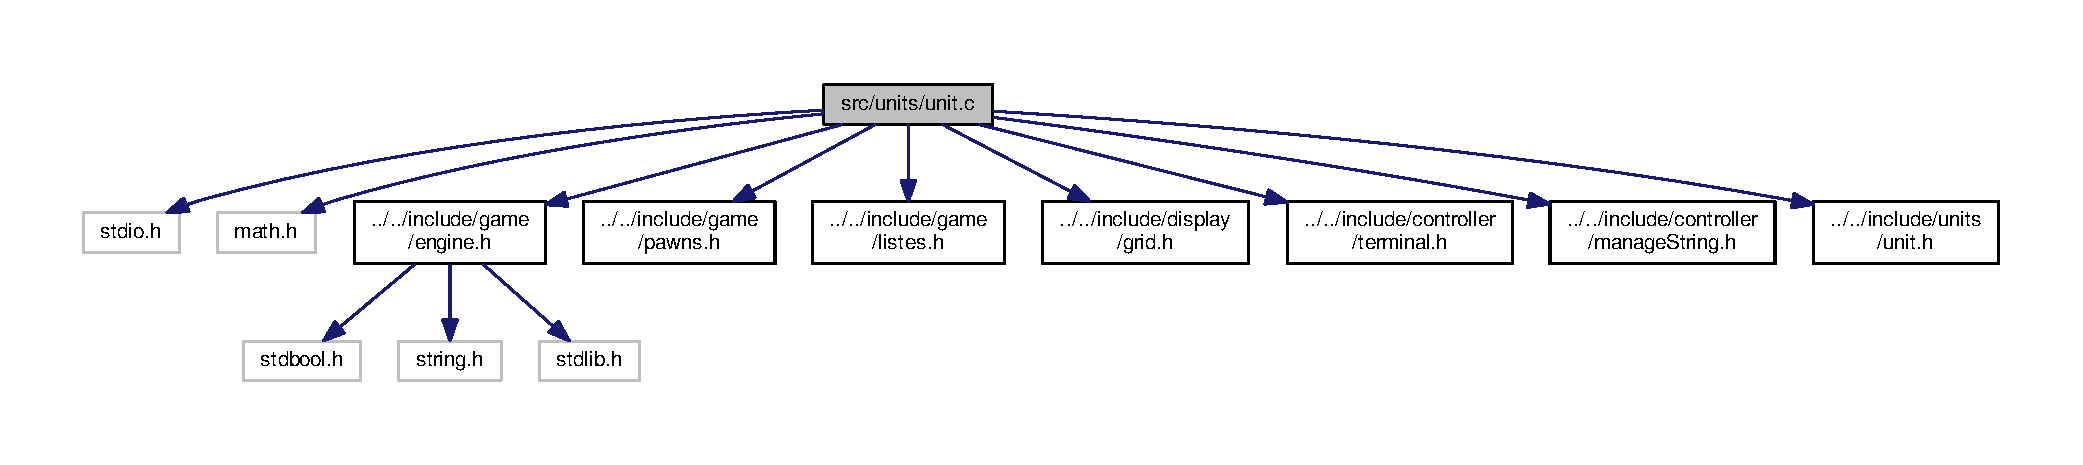
\includegraphics[width=350pt]{unit_8c__incl}
\end{center}
\end{figure}
\subsection*{Fonctions}
\begin{DoxyCompactItemize}
\item 
void \hyperlink{unit_8c_a303ffa342493b2383462975ee73371ff}{unit\+Init} (short no\+P, \hyperlink{structvector}{vector} coord\+Unit)
\begin{DoxyCompactList}\small\item\em Initialise l\textquotesingle{}unité courante. \end{DoxyCompactList}\item 
bool \hyperlink{unit_8c_a85f8dfae2c8d83d9bc1b164adac6513d}{can\+Get\+Passed} (\hyperlink{structunit}{unit} $\ast$target)
\begin{DoxyCompactList}\small\item\em Définis si le passage est permis. \end{DoxyCompactList}\item 
bool \hyperlink{unit_8c_ac194fc19a706dbd87e9a93c02b244f11}{can\+Block} (\hyperlink{structunit}{unit} $\ast$target)
\begin{DoxyCompactList}\small\item\em Définis si une unité peut bloquer. \end{DoxyCompactList}\item 
bool \hyperlink{unit_8c_aa012dba081af99c4a666767c26ac1ac5}{can\+Attack} (\hyperlink{structunit}{unit} $\ast$target)
\begin{DoxyCompactList}\small\item\em Définis si une unité peut attaquer. \end{DoxyCompactList}\item 
bool \hyperlink{unit_8c_a9c0738de90650e2f4640cae3bad4b3a2}{can\+Move} (\hyperlink{structunit}{unit} $\ast$target)
\begin{DoxyCompactList}\small\item\em Définis si une unité peut bouger. \end{DoxyCompactList}\item 
bool \hyperlink{unit_8c_a52de919c7103012ce231d80e3bbe3e8d}{can\+Teleport} (\hyperlink{engine_8h_af7667555c2dcfbdd55ec3e9dd6a907ba}{unit\+Name} name)
\begin{DoxyCompactList}\small\item\em Détermine si une unité peut se téléporter. \end{DoxyCompactList}\item 
void \hyperlink{unit_8c_a59537e7d55fc495b394087bf8a952d16}{heal} (\hyperlink{engine_8h_af7667555c2dcfbdd55ec3e9dd6a907ba}{unit\+Name} name)
\begin{DoxyCompactList}\small\item\em Soigne les unités. \end{DoxyCompactList}\item 
int \hyperlink{unit_8c_a5c8761ef40c541d75de80d6f6eeeb482}{get\+Side\+Attacked} (\hyperlink{structvector}{vector} source, \hyperlink{structvector}{vector} target)
\begin{DoxyCompactList}\small\item\em Retourne le côté attaqué \end{DoxyCompactList}\item 
void \hyperlink{unit_8c_a6b948a17bbc3106f230c32a53121e6db}{attack} (\hyperlink{structvector}{vector} source, \hyperlink{structvector}{vector} target)
\begin{DoxyCompactList}\small\item\em Attaque une unité en prenant en compte son taux de blocage. \end{DoxyCompactList}\item 
bool \hyperlink{unit_8c_a4004486abf500173fd3f51d2d3283275}{copy} (\hyperlink{structunit}{unit} $\ast$destination, \hyperlink{structunit}{unit} $\ast$source)
\begin{DoxyCompactList}\small\item\em Copie la structure source vers la structure destination. \end{DoxyCompactList}\item 
void \hyperlink{unit_8c_a27d0834cb55fab6867ffb3888c506d39}{erase} (\hyperlink{structunit}{unit} $\ast$source)
\begin{DoxyCompactList}\small\item\em Efface une unité de la grille. \end{DoxyCompactList}\item 
void \hyperlink{unit_8c_a4ea1b739c4b88857675c47d9960a69a4}{power\+Bonus} ()
\begin{DoxyCompactList}\small\item\em Octroie un bonus de puissance. \end{DoxyCompactList}\item 
void \hyperlink{unit_8c_a87c06ff9e86d3317e10387a5d5626f1a}{move} (\hyperlink{structvector}{vector} destination, \hyperlink{structvector}{vector} source)
\begin{DoxyCompactList}\small\item\em Déplace une unité vers la destination. \end{DoxyCompactList}\item 
void \hyperlink{unit_8c_a2fdda888eb5b942249418b75a4998581}{set\+Direction} (\hyperlink{structvector}{vector} source, int dir)
\begin{DoxyCompactList}\small\item\em Définis la direction de l\textquotesingle{}unité \end{DoxyCompactList}\item 
void \hyperlink{unit_8c_afec10f9e98c70ab1915023cd0c8f76ca}{poison} ()
\begin{DoxyCompactList}\small\item\em Gère le statut empoisonnement. \end{DoxyCompactList}\item 
void \hyperlink{unit_8c_ae52638eb8e2a94d1dd3df42c816681a3}{add\+Effect} (\hyperlink{structvector}{vector} target, \hyperlink{engine_8h_ac5ece9b6993cd3565502866b56317e84}{unit\+Effect} effect)
\begin{DoxyCompactList}\small\item\em Ajoute un effect sur l\textquotesingle{}unité cible. \end{DoxyCompactList}\item 
void \hyperlink{unit_8c_a1cbe53dd582c7ac03bafb0051a38a98b}{minus\+Effect} ()
\begin{DoxyCompactList}\small\item\em Décrémente les effets. \end{DoxyCompactList}\item 
void \hyperlink{unit_8c_ae887bebca3eb165cbbd7f71975cf8f3a}{sleep} (\hyperlink{structvector}{vector} pos)
\begin{DoxyCompactList}\small\item\em Endors l\textquotesingle{}unité \end{DoxyCompactList}\item 
bool \hyperlink{unit_8c_aa2bac651e557f022a73099db0185eb44}{is\+Sleeping} (\hyperlink{structvector}{vector} pos)
\begin{DoxyCompactList}\small\item\em Vérifie si l\textquotesingle{}unité est endormie. \end{DoxyCompactList}\item 
void \hyperlink{unit_8c_a505f360905b4ad0fa6e18f19405539ea}{recover} ()
\begin{DoxyCompactList}\small\item\em Réveille l\textquotesingle{}unité tour par tour. \end{DoxyCompactList}\item 
bool \hyperlink{unit_8c_a04cb7c9ee636e575bfd9531780b829d7}{all\+Static} (int num\+Player)
\begin{DoxyCompactList}\small\item\em Vérifie si toutes les unités sont immobilisés. \end{DoxyCompactList}\end{DoxyCompactItemize}


\subsection{Description détaillée}
Gestion des unités. 

\begin{DoxyAuthor}{Auteur}
Cousin Brandon Chaudemanche Ewen Biardeau Tristan 
\end{DoxyAuthor}
\begin{DoxyVersion}{Version}
v1.\+00 
\end{DoxyVersion}
\begin{DoxyDate}{Date}
18/12/2015 
\end{DoxyDate}


\subsection{Documentation des fonctions}
\hypertarget{unit_8c_ae52638eb8e2a94d1dd3df42c816681a3}{}\index{unit.\+c@{unit.\+c}!add\+Effect@{add\+Effect}}
\index{add\+Effect@{add\+Effect}!unit.\+c@{unit.\+c}}
\subsubsection[{add\+Effect}]{\setlength{\rightskip}{0pt plus 5cm}void add\+Effect (
\begin{DoxyParamCaption}
\item[{{\bf vector}}]{target, }
\item[{{\bf unit\+Effect}}]{effect}
\end{DoxyParamCaption}
)}\label{unit_8c_ae52638eb8e2a94d1dd3df42c816681a3}


Ajoute un effect sur l\textquotesingle{}unité cible. 

Ajoute un effet à une unité


\begin{DoxyParams}{Paramètres}
{\em target} & Position unité cible \\
\hline
{\em effect} & Effet à appliquer sur la cible \\
\hline
\end{DoxyParams}


Définition à la ligne 437 du fichier unit.\+c.

\hypertarget{unit_8c_a04cb7c9ee636e575bfd9531780b829d7}{}\index{unit.\+c@{unit.\+c}!all\+Static@{all\+Static}}
\index{all\+Static@{all\+Static}!unit.\+c@{unit.\+c}}
\subsubsection[{all\+Static}]{\setlength{\rightskip}{0pt plus 5cm}bool all\+Static (
\begin{DoxyParamCaption}
\item[{int}]{num\+Player}
\end{DoxyParamCaption}
)}\label{unit_8c_a04cb7c9ee636e575bfd9531780b829d7}


Vérifie si toutes les unités sont immobilisés. 

Vérifie si toutes les unités sont immobilisées.


\begin{DoxyParams}{Paramètres}
{\em num\+Player} & Numéro du joueur \\
\hline
\end{DoxyParams}
\begin{DoxyReturn}{Renvoie}
Retourne vrai si toutes les unités sont immobilisés 
\end{DoxyReturn}


Définition à la ligne 529 du fichier unit.\+c.

\hypertarget{unit_8c_a6b948a17bbc3106f230c32a53121e6db}{}\index{unit.\+c@{unit.\+c}!attack@{attack}}
\index{attack@{attack}!unit.\+c@{unit.\+c}}
\subsubsection[{attack}]{\setlength{\rightskip}{0pt plus 5cm}void attack (
\begin{DoxyParamCaption}
\item[{{\bf vector}}]{source, }
\item[{{\bf vector}}]{target}
\end{DoxyParamCaption}
)}\label{unit_8c_a6b948a17bbc3106f230c32a53121e6db}


Attaque une unité en prenant en compte son taux de blocage. 

Attaque une unité


\begin{DoxyParams}{Paramètres}
{\em source} & Unité attaquante \\
\hline
{\em target} & Unité cible \\
\hline
\end{DoxyParams}


Définition à la ligne 184 du fichier unit.\+c.

\hypertarget{unit_8c_aa012dba081af99c4a666767c26ac1ac5}{}\index{unit.\+c@{unit.\+c}!can\+Attack@{can\+Attack}}
\index{can\+Attack@{can\+Attack}!unit.\+c@{unit.\+c}}
\subsubsection[{can\+Attack}]{\setlength{\rightskip}{0pt plus 5cm}bool can\+Attack (
\begin{DoxyParamCaption}
\item[{{\bf unit} $\ast$}]{target}
\end{DoxyParamCaption}
)}\label{unit_8c_aa012dba081af99c4a666767c26ac1ac5}


Définis si une unité peut attaquer. 

Vérifie si l\textquotesingle{}unité peut attaquer.


\begin{DoxyParams}{Paramètres}
{\em target} & Unité à analyser \\
\hline
\end{DoxyParams}
\begin{DoxyReturn}{Renvoie}
Retourne vrai si l\textquotesingle{}unité peut attaquer 
\end{DoxyReturn}


Définition à la ligne 86 du fichier unit.\+c.

\hypertarget{unit_8c_ac194fc19a706dbd87e9a93c02b244f11}{}\index{unit.\+c@{unit.\+c}!can\+Block@{can\+Block}}
\index{can\+Block@{can\+Block}!unit.\+c@{unit.\+c}}
\subsubsection[{can\+Block}]{\setlength{\rightskip}{0pt plus 5cm}bool can\+Block (
\begin{DoxyParamCaption}
\item[{{\bf unit} $\ast$}]{target}
\end{DoxyParamCaption}
)}\label{unit_8c_ac194fc19a706dbd87e9a93c02b244f11}


Définis si une unité peut bloquer. 

Vérifie si l\textquotesingle{}unité peut bloquer.


\begin{DoxyParams}{Paramètres}
{\em target} & Unité à analyser \\
\hline
\end{DoxyParams}
\begin{DoxyReturn}{Renvoie}
Retourne vrai si l\textquotesingle{}unité peut bloquer 
\end{DoxyReturn}


Définition à la ligne 66 du fichier unit.\+c.

\hypertarget{unit_8c_a85f8dfae2c8d83d9bc1b164adac6513d}{}\index{unit.\+c@{unit.\+c}!can\+Get\+Passed@{can\+Get\+Passed}}
\index{can\+Get\+Passed@{can\+Get\+Passed}!unit.\+c@{unit.\+c}}
\subsubsection[{can\+Get\+Passed}]{\setlength{\rightskip}{0pt plus 5cm}bool can\+Get\+Passed (
\begin{DoxyParamCaption}
\item[{{\bf unit} $\ast$}]{target}
\end{DoxyParamCaption}
)}\label{unit_8c_a85f8dfae2c8d83d9bc1b164adac6513d}


Définis si le passage est permis. 

Vérifie si le passage est autorisé


\begin{DoxyParams}{Paramètres}
{\em target} & Unité à analyser \\
\hline
\end{DoxyParams}
\begin{DoxyReturn}{Renvoie}
Retourne vrai si passage autorisé 
\end{DoxyReturn}


Définition à la ligne 46 du fichier unit.\+c.

\hypertarget{unit_8c_a9c0738de90650e2f4640cae3bad4b3a2}{}\index{unit.\+c@{unit.\+c}!can\+Move@{can\+Move}}
\index{can\+Move@{can\+Move}!unit.\+c@{unit.\+c}}
\subsubsection[{can\+Move}]{\setlength{\rightskip}{0pt plus 5cm}bool can\+Move (
\begin{DoxyParamCaption}
\item[{{\bf unit} $\ast$}]{target}
\end{DoxyParamCaption}
)}\label{unit_8c_a9c0738de90650e2f4640cae3bad4b3a2}


Définis si une unité peut bouger. 

Vérifie si l\textquotesingle{}unité peut bouger.


\begin{DoxyParams}{Paramètres}
{\em target} & Unité à analyser \\
\hline
\end{DoxyParams}
\begin{DoxyReturn}{Renvoie}
Retourne vraie si l\textquotesingle{}unité peut se mouvoir 
\end{DoxyReturn}


Définition à la ligne 106 du fichier unit.\+c.

\hypertarget{unit_8c_a52de919c7103012ce231d80e3bbe3e8d}{}\index{unit.\+c@{unit.\+c}!can\+Teleport@{can\+Teleport}}
\index{can\+Teleport@{can\+Teleport}!unit.\+c@{unit.\+c}}
\subsubsection[{can\+Teleport}]{\setlength{\rightskip}{0pt plus 5cm}bool can\+Teleport (
\begin{DoxyParamCaption}
\item[{{\bf unit\+Name}}]{name}
\end{DoxyParamCaption}
)}\label{unit_8c_a52de919c7103012ce231d80e3bbe3e8d}


Détermine si une unité peut se téléporter. 

Vérifie si l\textquotesingle{}unité peut se téléporter.


\begin{DoxyParams}{Paramètres}
{\em name} & Nom de l\textquotesingle{}unité \\
\hline
\end{DoxyParams}
\begin{DoxyReturn}{Renvoie}
Retourne vraie si l\textquotesingle{}unité peut se déplacer 
\end{DoxyReturn}


Définition à la ligne 125 du fichier unit.\+c.

\hypertarget{unit_8c_a4004486abf500173fd3f51d2d3283275}{}\index{unit.\+c@{unit.\+c}!copy@{copy}}
\index{copy@{copy}!unit.\+c@{unit.\+c}}
\subsubsection[{copy}]{\setlength{\rightskip}{0pt plus 5cm}bool copy (
\begin{DoxyParamCaption}
\item[{{\bf unit} $\ast$}]{destination, }
\item[{{\bf unit} $\ast$}]{source}
\end{DoxyParamCaption}
)}\label{unit_8c_a4004486abf500173fd3f51d2d3283275}


Copie la structure source vers la structure destination. 

Copie la structure source vers destination.


\begin{DoxyParams}{Paramètres}
{\em destination} & Structure destination \\
\hline
{\em source} & Structure source \\
\hline
\end{DoxyParams}
\begin{DoxyReturn}{Renvoie}
Retourne vrai si copie bien déroulée 
\end{DoxyReturn}


Définition à la ligne 236 du fichier unit.\+c.

\hypertarget{unit_8c_a27d0834cb55fab6867ffb3888c506d39}{}\index{unit.\+c@{unit.\+c}!erase@{erase}}
\index{erase@{erase}!unit.\+c@{unit.\+c}}
\subsubsection[{erase}]{\setlength{\rightskip}{0pt plus 5cm}void erase (
\begin{DoxyParamCaption}
\item[{{\bf unit} $\ast$}]{source}
\end{DoxyParamCaption}
)}\label{unit_8c_a27d0834cb55fab6867ffb3888c506d39}


Efface une unité de la grille. 


\begin{DoxyParams}{Paramètres}
{\em source} & Source à effacer \\
\hline
\end{DoxyParams}


Définition à la ligne 271 du fichier unit.\+c.

\hypertarget{unit_8c_a5c8761ef40c541d75de80d6f6eeeb482}{}\index{unit.\+c@{unit.\+c}!get\+Side\+Attacked@{get\+Side\+Attacked}}
\index{get\+Side\+Attacked@{get\+Side\+Attacked}!unit.\+c@{unit.\+c}}
\subsubsection[{get\+Side\+Attacked}]{\setlength{\rightskip}{0pt plus 5cm}int get\+Side\+Attacked (
\begin{DoxyParamCaption}
\item[{{\bf vector}}]{source, }
\item[{{\bf vector}}]{target}
\end{DoxyParamCaption}
)}\label{unit_8c_a5c8761ef40c541d75de80d6f6eeeb482}


Retourne le côté attaqué 

Récupère le côté attaqué


\begin{DoxyParams}{Paramètres}
{\em source} & Position unité source \\
\hline
{\em target} & Position unité cible \\
\hline
\end{DoxyParams}
\begin{DoxyReturn}{Renvoie}
Le côté attaqué 
\end{DoxyReturn}


Définition à la ligne 168 du fichier unit.\+c.

\hypertarget{unit_8c_a59537e7d55fc495b394087bf8a952d16}{}\index{unit.\+c@{unit.\+c}!heal@{heal}}
\index{heal@{heal}!unit.\+c@{unit.\+c}}
\subsubsection[{heal}]{\setlength{\rightskip}{0pt plus 5cm}void heal (
\begin{DoxyParamCaption}
\item[{{\bf unit\+Name}}]{name}
\end{DoxyParamCaption}
)}\label{unit_8c_a59537e7d55fc495b394087bf8a952d16}


Soigne les unités. 


\begin{DoxyParams}{Paramètres}
{\em name} & Nom de l\textquotesingle{}unité soignant \\
\hline
\end{DoxyParams}


Définition à la ligne 137 du fichier unit.\+c.

\hypertarget{unit_8c_aa2bac651e557f022a73099db0185eb44}{}\index{unit.\+c@{unit.\+c}!is\+Sleeping@{is\+Sleeping}}
\index{is\+Sleeping@{is\+Sleeping}!unit.\+c@{unit.\+c}}
\subsubsection[{is\+Sleeping}]{\setlength{\rightskip}{0pt plus 5cm}bool is\+Sleeping (
\begin{DoxyParamCaption}
\item[{{\bf vector}}]{pos}
\end{DoxyParamCaption}
)}\label{unit_8c_aa2bac651e557f022a73099db0185eb44}


Vérifie si l\textquotesingle{}unité est endormie. 

Vérifie si une unité est endormie.


\begin{DoxyParams}{Paramètres}
{\em pos} & Position de l\textquotesingle{}unité \\
\hline
\end{DoxyParams}
\begin{DoxyReturn}{Renvoie}
Retourne vrai si endormi 
\end{DoxyReturn}


Définition à la ligne 490 du fichier unit.\+c.

\hypertarget{unit_8c_a1cbe53dd582c7ac03bafb0051a38a98b}{}\index{unit.\+c@{unit.\+c}!minus\+Effect@{minus\+Effect}}
\index{minus\+Effect@{minus\+Effect}!unit.\+c@{unit.\+c}}
\subsubsection[{minus\+Effect}]{\setlength{\rightskip}{0pt plus 5cm}void minus\+Effect (
\begin{DoxyParamCaption}
{}
\end{DoxyParamCaption}
)}\label{unit_8c_a1cbe53dd582c7ac03bafb0051a38a98b}


Décrémente les effets. 

Diminue le temps de l\textquotesingle{}effet. 

Définition à la ligne 455 du fichier unit.\+c.

\hypertarget{unit_8c_a87c06ff9e86d3317e10387a5d5626f1a}{}\index{unit.\+c@{unit.\+c}!move@{move}}
\index{move@{move}!unit.\+c@{unit.\+c}}
\subsubsection[{move}]{\setlength{\rightskip}{0pt plus 5cm}void move (
\begin{DoxyParamCaption}
\item[{{\bf vector}}]{destination, }
\item[{{\bf vector}}]{source}
\end{DoxyParamCaption}
)}\label{unit_8c_a87c06ff9e86d3317e10387a5d5626f1a}


Déplace une unité vers la destination. 

Bouge une unité


\begin{DoxyParams}{Paramètres}
{\em destination} & Destination souhaitée \\
\hline
{\em source} & Position de l\textquotesingle{}unité \\
\hline
\end{DoxyParams}


Définition à la ligne 351 du fichier unit.\+c.

\hypertarget{unit_8c_afec10f9e98c70ab1915023cd0c8f76ca}{}\index{unit.\+c@{unit.\+c}!poison@{poison}}
\index{poison@{poison}!unit.\+c@{unit.\+c}}
\subsubsection[{poison}]{\setlength{\rightskip}{0pt plus 5cm}void poison (
\begin{DoxyParamCaption}
{}
\end{DoxyParamCaption}
)}\label{unit_8c_afec10f9e98c70ab1915023cd0c8f76ca}


Gère le statut empoisonnement. 

Empoisonne une unité 

Définition à la ligne 386 du fichier unit.\+c.

\hypertarget{unit_8c_a4ea1b739c4b88857675c47d9960a69a4}{}\index{unit.\+c@{unit.\+c}!power\+Bonus@{power\+Bonus}}
\index{power\+Bonus@{power\+Bonus}!unit.\+c@{unit.\+c}}
\subsubsection[{power\+Bonus}]{\setlength{\rightskip}{0pt plus 5cm}void power\+Bonus (
\begin{DoxyParamCaption}
{}
\end{DoxyParamCaption}
)}\label{unit_8c_a4ea1b739c4b88857675c47d9960a69a4}


Octroie un bonus de puissance. 

Octroie un bonus de puissance selon certaines conditions. 

Définition à la ligne 286 du fichier unit.\+c.

\hypertarget{unit_8c_a505f360905b4ad0fa6e18f19405539ea}{}\index{unit.\+c@{unit.\+c}!recover@{recover}}
\index{recover@{recover}!unit.\+c@{unit.\+c}}
\subsubsection[{recover}]{\setlength{\rightskip}{0pt plus 5cm}void recover (
\begin{DoxyParamCaption}
{}
\end{DoxyParamCaption}
)}\label{unit_8c_a505f360905b4ad0fa6e18f19405539ea}


Réveille l\textquotesingle{}unité tour par tour. 

Se réveille tour par tour. 

Définition à la ligne 503 du fichier unit.\+c.

\hypertarget{unit_8c_a2fdda888eb5b942249418b75a4998581}{}\index{unit.\+c@{unit.\+c}!set\+Direction@{set\+Direction}}
\index{set\+Direction@{set\+Direction}!unit.\+c@{unit.\+c}}
\subsubsection[{set\+Direction}]{\setlength{\rightskip}{0pt plus 5cm}void set\+Direction (
\begin{DoxyParamCaption}
\item[{{\bf vector}}]{source, }
\item[{int}]{dir}
\end{DoxyParamCaption}
)}\label{unit_8c_a2fdda888eb5b942249418b75a4998581}


Définis la direction de l\textquotesingle{}unité 

Définis la direction d\textquotesingle{}une unité


\begin{DoxyParams}{Paramètres}
{\em source} & Unité à tourner \\
\hline
{\em dir} & Direction dans laquelle tourner \\
\hline
\end{DoxyParams}


Définition à la ligne 377 du fichier unit.\+c.

\hypertarget{unit_8c_ae887bebca3eb165cbbd7f71975cf8f3a}{}\index{unit.\+c@{unit.\+c}!sleep@{sleep}}
\index{sleep@{sleep}!unit.\+c@{unit.\+c}}
\subsubsection[{sleep}]{\setlength{\rightskip}{0pt plus 5cm}void sleep (
\begin{DoxyParamCaption}
\item[{{\bf vector}}]{pos}
\end{DoxyParamCaption}
)}\label{unit_8c_ae887bebca3eb165cbbd7f71975cf8f3a}


Endors l\textquotesingle{}unité 

Endors une unité


\begin{DoxyParams}{Paramètres}
{\em pos} & Position de l\textquotesingle{}unité \\
\hline
\end{DoxyParams}


Définition à la ligne 480 du fichier unit.\+c.

\hypertarget{unit_8c_a303ffa342493b2383462975ee73371ff}{}\index{unit.\+c@{unit.\+c}!unit\+Init@{unit\+Init}}
\index{unit\+Init@{unit\+Init}!unit.\+c@{unit.\+c}}
\subsubsection[{unit\+Init}]{\setlength{\rightskip}{0pt plus 5cm}void unit\+Init (
\begin{DoxyParamCaption}
\item[{short}]{no\+P, }
\item[{{\bf vector}}]{coord\+Unit}
\end{DoxyParamCaption}
)}\label{unit_8c_a303ffa342493b2383462975ee73371ff}


Initialise l\textquotesingle{}unité courante. 

Initialise une unité


\begin{DoxyParams}{Paramètres}
{\em no\+P} & Numéro du joueur \\
\hline
{\em coord\+Unit} & Coordonnées de l\textquotesingle{}unité \\
\hline
\end{DoxyParams}


Définition à la ligne 24 du fichier unit.\+c.


%--- End generated contents ---

% Index
\backmatter
\newpage
\phantomsection
\clearemptydoublepage
\addcontentsline{toc}{chapter}{Index}
\printindex

\end{document}
